\documentclass[10pt]{article}
\usepackage[utf8]{inputenc}
\usepackage{geometry}
\usepackage{amsfonts}
\usepackage{hyperref}
\usepackage{enumitem}
\usepackage{graphicx}
\usepackage{tabularx}
\usepackage{amsmath}
\usepackage{xcolor}


\title{
    \textbf{CSE344: Computer Vision} \\ \vspace*{-5pt}
    \textbf{\large{Assignment-1}}
}

\author{\href{mailto:divyajeet21529@iiitd.ac.in}{Divyajeet Singh (2021529)}}
\date{\today}

\geometry{a4paper, left=20mm, right=20mm, top=20mm, bottom=20mm}


\begin{document}
    \maketitle

    \section*{\textbf{Theory}}

    \subsection*{\textbf{Question 1.}}
    \begin{enumerate}[label=(\alph*)]
        \item The given problem of classifying papaya images into the classes `sweet'
        and `not sweet' is a binary classification problem. The Mean Squared Error function
        is non-convex for binary classifcation. Thus if a binary classifier is
        trained with MSE Loss, it is not guaranteed to converege to the minimum of the loss.
        Secondly, using MSE assumes an underlying Gaussian distribution\footnote{
        In fact, mean squared error is the KL divergence between the empirical distribution of
        the data and a Gaussian model.},
        which is not valid in case of binary classification, since it is modeled with a
        Bernoulli distribution.

        \item For a single training example, the Binary Cross Entropy loss function
        is given by (assuming $\hat{y}$ is a valid probability in $[0, 1]$)
        \begin{equation*}
            \mathcal{L}(\hat{y}) = - y \log_{2}{(\hat{y})} - (1 - y) \log_{2}{(1 - \hat{y})}
        \end{equation*}

        \item On a negative example (where $y = 0$), if the predicted value is $\hat{y} = 0.9$,
        the value of loss is given by
        \begin{equation*}
            \mathcal{L}(0.9) = - 0 \log_{2}{(0.9)} - (1 - 0) \log_{2}{(1 - 0.9)}
            = - \log_{2}{(0.1)} \approx 3.322
        \end{equation*}

        \item Now, we calculate the mean loss for 3 examples for the given ground truth
        and predicted values
        \begin{align*}
            \mathcal{L}(\hat{Y}) &= - \frac{1}{3} \sum_{i=1}^{3} y_{i} \log_{2}{\hat{y_{i}}} +
            (1 - y_{i}) \log_{2}{(1 - \hat{y_{i}})} \\
            &= - \frac{1}{3} \big{(} \log_{2}{(0.1)} + \log_{2}{(0.8)} + \log_{2}{(0.3)} \big{)} \\
            &\approx \frac{1}{3} \big{(} 3.322 + 0.322 + 1.737 \big{)} = \frac{5.381}{3} \approx 1.793
        \end{align*}

        \item For a learning rate $\alpha$ and a traininable weight $W$, the update formula
        while using $L_{2}$-regularization (hyperparameter $\lambda$) is given by
        \begin{equation*}
            W_{\mathbf{new}} \gets W_{\mathbf{old}} - \alpha \left( \frac{\partial{L_{BCE}}}{\partial{W}}
            + 2 \lambda W_{\mathbf{old}} \right)
        \end{equation*}
        The $L_{2}$-regularization applied in model $A$ penalizes very large weights by adding some
        proportion of the weights themselves to the gradient update. Hence, we expect model $A$'s weights
        to be relatively smaller than model $B$'s final trained weights. However, this technique (usually)
        reduces overfitting, as model $A$ will be encouraged to learn simpler patterns than model $B$.

        \item KL-divergence is a measure of `\textit{distance}' or difference between two probability distributions.
        KL-divergence measures the relative entropy of two distributions. On the other hand, cross entropy can
        be thought of as the total entropy between them. The formula for KL-divergence and cross-entropy are as follows
        \begin{align*}
            D_{\text{KL}}(P || Q) = \mathbb{E}_{X \sim P}\left[ \log\frac{P(X)}{Q(X)} \right]
            &= \mathbb{E}_{X \sim P}[\log P(X) - \log Q(X)]\\
            H(P, Q) &= - \mathbb{E}_{X \sim P}[\log Q(X)]
        \end{align*}
        These quantities are closely related - minimizing the cross-entropy $H(P, Q)$ with respect to $Q$
        is equivalent to minimize the KL-divergence $D_{\text{KL}}(P || Q)$. Their relationship is given in
        the following equations
        \begin{align*}
            D_{\text{KL}}(P || Q) &= \mathbb{E}_{X \sim P}[\log P(X)] - \mathbb{E}_{X \sim P}[\log Q(X)] \\
            &= H(P, Q) + \mathbb{E}_{X \sim P}[\log P(X)] \\
            &= H(P, Q) - H(P) \\
            \implies H(P, Q) &= H(P) + D_{\text{KL}}(P || Q)
        \end{align*}
        where Shannon entropy of a distribution $P$ is defined as in class,
        \begin{equation*}
            H(P) = - \mathbb{E}_{X \sim P}[\log P(X)]
        \end{equation*}
    \end{enumerate}

    \subsection*{\textbf{Question 2.}}
    We are given the following information about the 2-layer neural network for
    $K$-class classification problem.
    \begin{align*}
        z^{[i]} &= W^{[i]} a^{[i-1]} + b^{[i]}, \quad i = 1, 2 \quad a^{[0]} = x \\
        a^{[1]} &= \textsc{LeakyReLU}\left( z^{[1]}, \alpha=10^{-2} \right) \\
        \hat{y} &= \textsc{Softmax}\left( z^{[2]} \right) = \sigma\left( z^{[2]} \right) \quad \text{(say)} \\
        \mathcal{L}(\hat{y}) &= - \sum_{i=1}^{K} y_{i} \log{(\hat{y_{i}})}
    \end{align*}
    \begin{enumerate}[label=(\alph*)]
        \item Let us assume $z^{[2]}$ is of size $K \times 1$ (since it is a $K$-class
        classification problem). Since $z^{[1]}$ is of size $D_{a} \times 1$, $a^{[1]}$
        must be of the same size, and hence, the $W^{[2]}$ must of be size $K \times D_{a}$.
        Following this, $b^{[2]}$ must be of size $K \times 1$.
        \begin{equation*}
            \underbrace{z^{[2]}}_{K \times 1} = \underbrace{W^{[2]}}_{K \times D_{a}} \
            \underbrace{a^{[1]}}_{D_{a} \times 1} + \underbrace{b^{[2]}}_{K \times 1}
        \end{equation*}
        By the same logic, $W^{[1]}$ must be of size $D_{a} \times D_{x}$, since the output $z^{[1]}$ must
        be of dimension $D_{a} \times 1$ while the input is of size $D_{x} \times 1$. \\
        Now, if we want to vectorize our input to a batch size of $m$, the input $X$ will be of
        size $D_{x} \times m$. This means that the output $z^{[1]}$ of the hidden layer will be
        $D_{a} \times m$, since
        \begin{equation*}
            \underbrace{z^{[1]}}_{D_{a} \times m} = \underbrace{W^{[1]}}_{D_{a} \times D_{x}} \
            \underbrace{X}_{D_{x} \times m} + \underbrace{b^{[1]}}_{D_{a} \times 1^{\textbf{*}}}
        \end{equation*}
        \textbf{*Note:} Bias is added component-wise to each column of $W^{[1]} X$ in case of
        vectorization of operations.

        \item Let us denote the sum of exponentials (normalizing term) of the entries in $z^{[2]}$ by
        \begin{align*}
            \mathbf{z} &= \sum_{j=1}^{K} \exp{z^{[2]}_{j}} \text{, which means } \hat{y} = \sigma\left( z^{[2]} \right) = \frac{\exp{z^{[2]}}}{\mathbf{z}}
        \end{align*}
        We are required to find the partial derivative of the $k^{th}$ entry in $\hat{y}$ with respect
        to the $k^{th}$ entry in $z^{[2]}$.
        \begin{align*}
            \frac{\partial{\hat{y}_{k}}}{\partial{z^{[2]}_{k}}} &= \frac{\partial}{\partial{z^{[2]}_{k}}} \left( \sigma\left( z^{[2]}_{k} \right) \right)
            = \frac{\partial}{\partial{z^{[2]}_{k}}} \left( \frac{\exp{z^{[2]}_{k}}}{\mathbf{z}} \right) \\
            &= \frac{1}{\mathbf{z}^{2}} \left( \mathbf{z} \ \frac{\partial}{\partial{z^{[2]}_{k}}} \left( \exp{z^{[2]}_{k}} \right) -
            \exp{z^{[2]}_{k}} \ \frac{\partial}{\partial{z^{[2]}_{k}}} \left( \mathbf{z} \right) \right) \\
            &= \frac{1}{\mathbf{z}^{2}} \left( \mathbf{z} \ \exp{z^{[2]}_{k}} \ - \ \left( \exp{z^{[2]}_{k}} \right)^{2} \right)
            = \frac{\exp{z^{[2]}_{k}}}{\mathbf{z}} - \left( \frac{\exp{z^{[2]}_{k}}}{\mathbf{z}} \right)^{2} \\
            &= \hat{y}_{k} - \hat{y}_{k}^{2} = \hat{y}_{k} \left( 1 - \hat{y}_{k} \right)
        \end{align*}

        \item Next, we find the partial derivative of the $k^{th}$ entry in $\hat{y}$ with respect
        to the $i^{th}$ entry in $z^{[2]}$, given $i \neq k$.
        \begin{align*}
            \frac{\partial{\hat{y}_{k}}}{\partial{z^{[2]}_{i}}} &= \frac{\partial}{\partial{z^{[2]}_{i}}} \left( \sigma\left( z^{[2]}_{k} \right) \right)
            = \frac{\partial}{\partial{z^{[2]}_{i}}} \left( \frac{\exp{z^{[2]}_{k}}}{\mathbf{z}} \right) \\
            &= \frac{1}{\mathbf{z}^{2}} \left( \mathbf{z} \ \frac{\partial}{\partial{z^{[2]}_{i}}} \left( \exp{z^{[2]}_{k}} \right) -
            \exp{z^{[2]}_{k}} \ \frac{\partial}{\partial{z^{[2]}_{i}}} \left( \mathbf{z} \right) \right) \\
            &= \frac{1}{\mathbf{z}^{2}} \left( 0 - \exp{z^{[2]}_{k}} \exp{z^{[2]}_{i}} \right)
            = - \frac{\exp{z^{[2]}_{k}}}{\mathbf{z}} \cdot \frac{\exp{z^{[2]}_{i}}}{\mathbf{z}} \\
            &= - \hat{y}_{k} \hat{y}_{i}
        \end{align*}

        \item We are interested in the partial derivative of the loss with respect to entries in $z^{[2]}$. Using
        the chain rule, we have
        \begin{equation*}
            \frac{\partial{\mathcal{L}}}{\partial{z^{[2]}_{i}}} =
            \frac{\partial{\mathcal{L}}}{\partial{\hat{y}_{i}}} \frac{\partial{\hat{y}_{i}}}{\partial{z^{[2]}_{i}}}
        \end{equation*}
        With the above (given) loss function, we can find
        \begin{equation*}
            \frac{\partial{\mathcal{L}}}{\partial{\hat{y}_{i}}}
            = \frac{\partial}{\partial{\hat{y}_{i}}} \left( -\sum_{j=1}^{K} y_{j} \log{(\hat{y}_{j})} \right)
            = -\sum_{j=1}^{K} y_{j} \frac{\partial}{\partial{\hat{y}_{i}}} (\log{(\hat{y}_{j})})
            = - \frac{y_{i}}{\hat{y}_{i}}
        \end{equation*}
        Note that as a result from \textbf{Question 2.} (b),
        \begin{equation*}
            \frac{\partial{\hat{y}_{i}}}{\partial{z^{[2]}_{i}}} = \hat{y}_{i} (1 - \hat{y}_{i})
        \end{equation*}
        So, we have
        \begin{equation*}
            \frac{\partial{\mathcal{L}}}{\partial{z^{[2]}_{i}}} = - \frac{y_{i}}{\hat{y}_{i}} \cdot \hat{y}_{i} (1 - \hat{y}_{i})
            = - y_{i} (1 - \hat{y}_{i})
        \end{equation*}
        Now, we are given that $y_{k} = 1$ and $y_{i} = 0, i \neq k$. So, we get (where $\mathbb{I}$ is an indicator variable)
        \begin{equation*}
            \frac{\partial{\mathcal{L}}}{\partial{z^{[2]}_{i}}} = \mathbb{I}_{\{i = k\}} (\hat{y_{i}} - 1) = \begin{cases}
                \hat{y}_{k} - 1 & \text{if } i = k \\
                0 & \text{if } i \neq k
            \end{cases}
        \end{equation*}

        \item While implementing the softmax function, we run into the problem of numerical overflow
        and underflow. Overflow occurs while exponentiating large numbers, when the result exceeds the
        computer's largest representable float value. In such cases, the result of $e^{z}$ is estimated to be
        infinity (\texttt{torch.inf} in PyTorch). Conversely, underflow occurs while exponentiating small
        numbers, when extremely small values are represented by zeros. Rarely, it is also possible
        that the denominator is extremely small, which makes division unstable. \\
        A common modification to resolve the issue is normalizing the input by max-shifting. In this
        technique, we subtract the maximum of the vector from all its entries, making all of them
        non-positive, and at least one entry 0. The output probabilities do not change because the relative
        difference between the entries in $z$ does not change, but the numberical
        operations become more stable. So, for a vector $z$ of size $m$, we get
        \begin{align*}
            z^{*} &= z - \max_{k = 1, 2, \dots, m}{z_{k}} \\
            \sigma(z) &= \sigma(z^{*}) = \frac{\exp{z^{*}}}{\sum_{j=1}^{m} \exp{z_{j}^{*}}}
        \end{align*}
    \end{enumerate}

    \section*{\textbf{Image Classification}}
    The solutions to the questions in this section are given in \texttt{classification.ipynb}.

    \subsection*{\textbf{Question 1.}}
    \begin{enumerate}[label=(\alph*)]
        \item The dataset was downloaded to my system from the Google Drive (I know, i
        couldn't figure out how to connect it to Google Colab and use GPU :sad:). The
        dataset was loaded using a custom class, \texttt{WildlifeDataset},
        which also handled the category to label mapping.
        \item The splits of ratio 0.7:0.1:0.2 were generated and loaded using dataloaders
        with batch size 256.
        \item To visualize the data distribution across class labels, we count the number
        of images in the entire dataset. Then, I compared the proportion of images in each
        class in the training and validation set. `Proportion' refers to the fraction of
        images of the entire dataset belonging to each class. The plots are given in the
        Figure (\ref{fig:classification-data-distro}) (Blue represents the training set and
        Orange represents the validation set).
        \begin{figure}[h!]
            \centering
            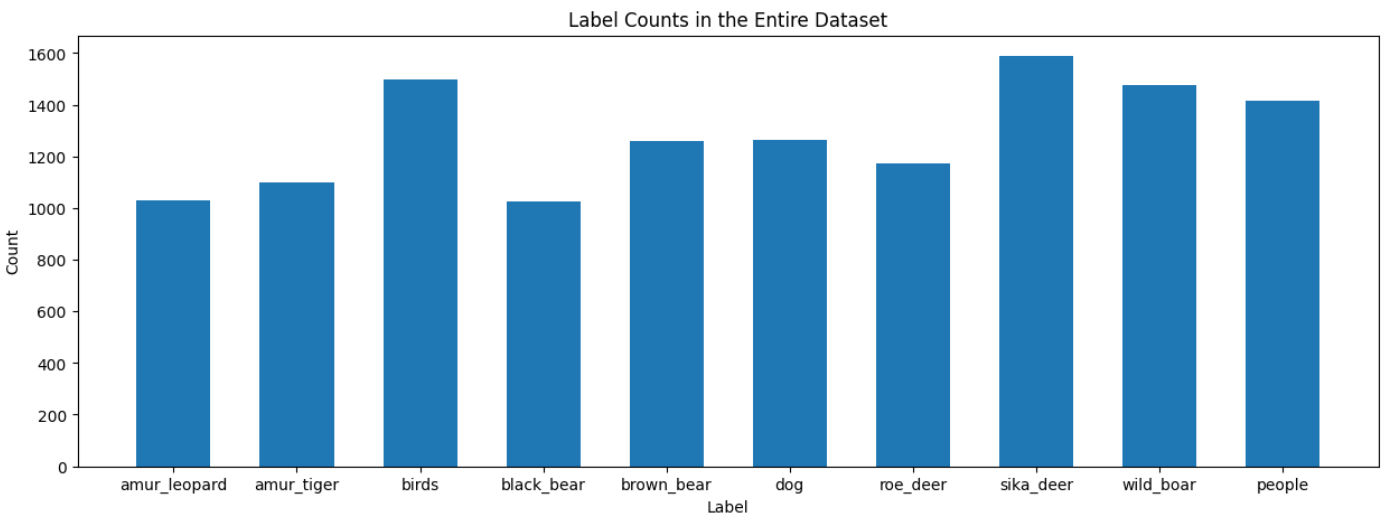
\includegraphics[width=0.7\textwidth]{Assets/Classification/01}
            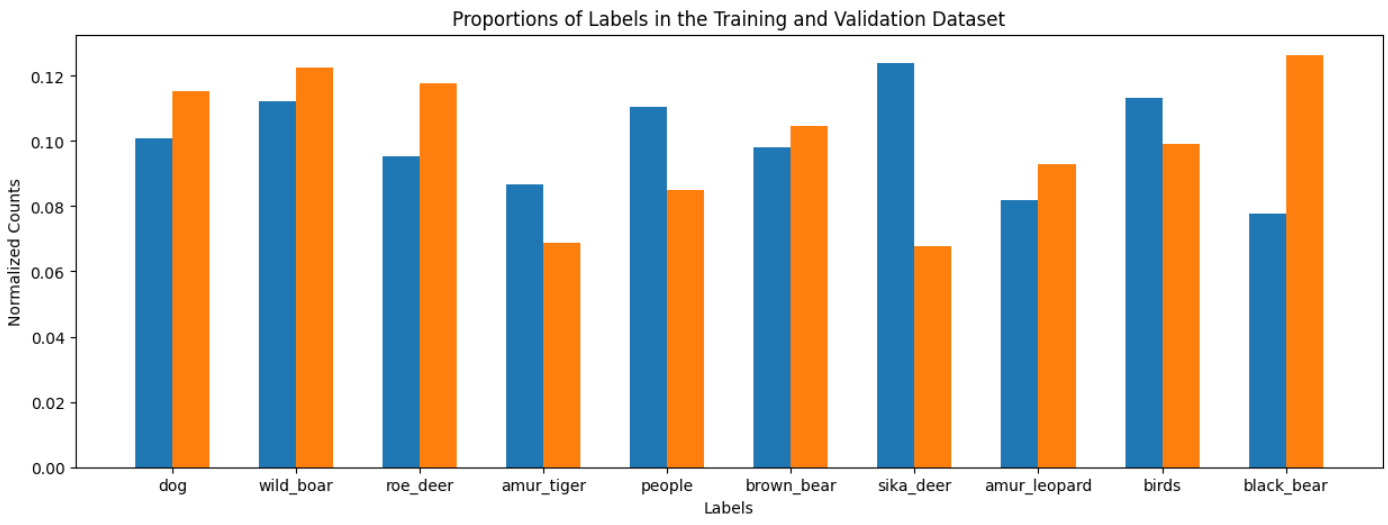
\includegraphics[width=0.7\textwidth]{Assets/Classification/02}
            \caption{Class distribution in the entire dataset, training set, and validation set}
            \label{fig:classification-data-distro}
        \end{figure}
    \end{enumerate}

    \subsection*{\textbf{Question 2.}}
    \begin{enumerate}[label=(\alph*)]
        \item The given CNN architecture was constructed in the class \texttt{ConvNet} using PyTorch
        and was trained for a total of 15 epochs.
        \item The per epoch loss/accuracy curves generated using wandb are given in Figure
        (\ref{fig:convnet-loss-accuracy-curves}).
        \begin{figure}[h!]
            \centering
            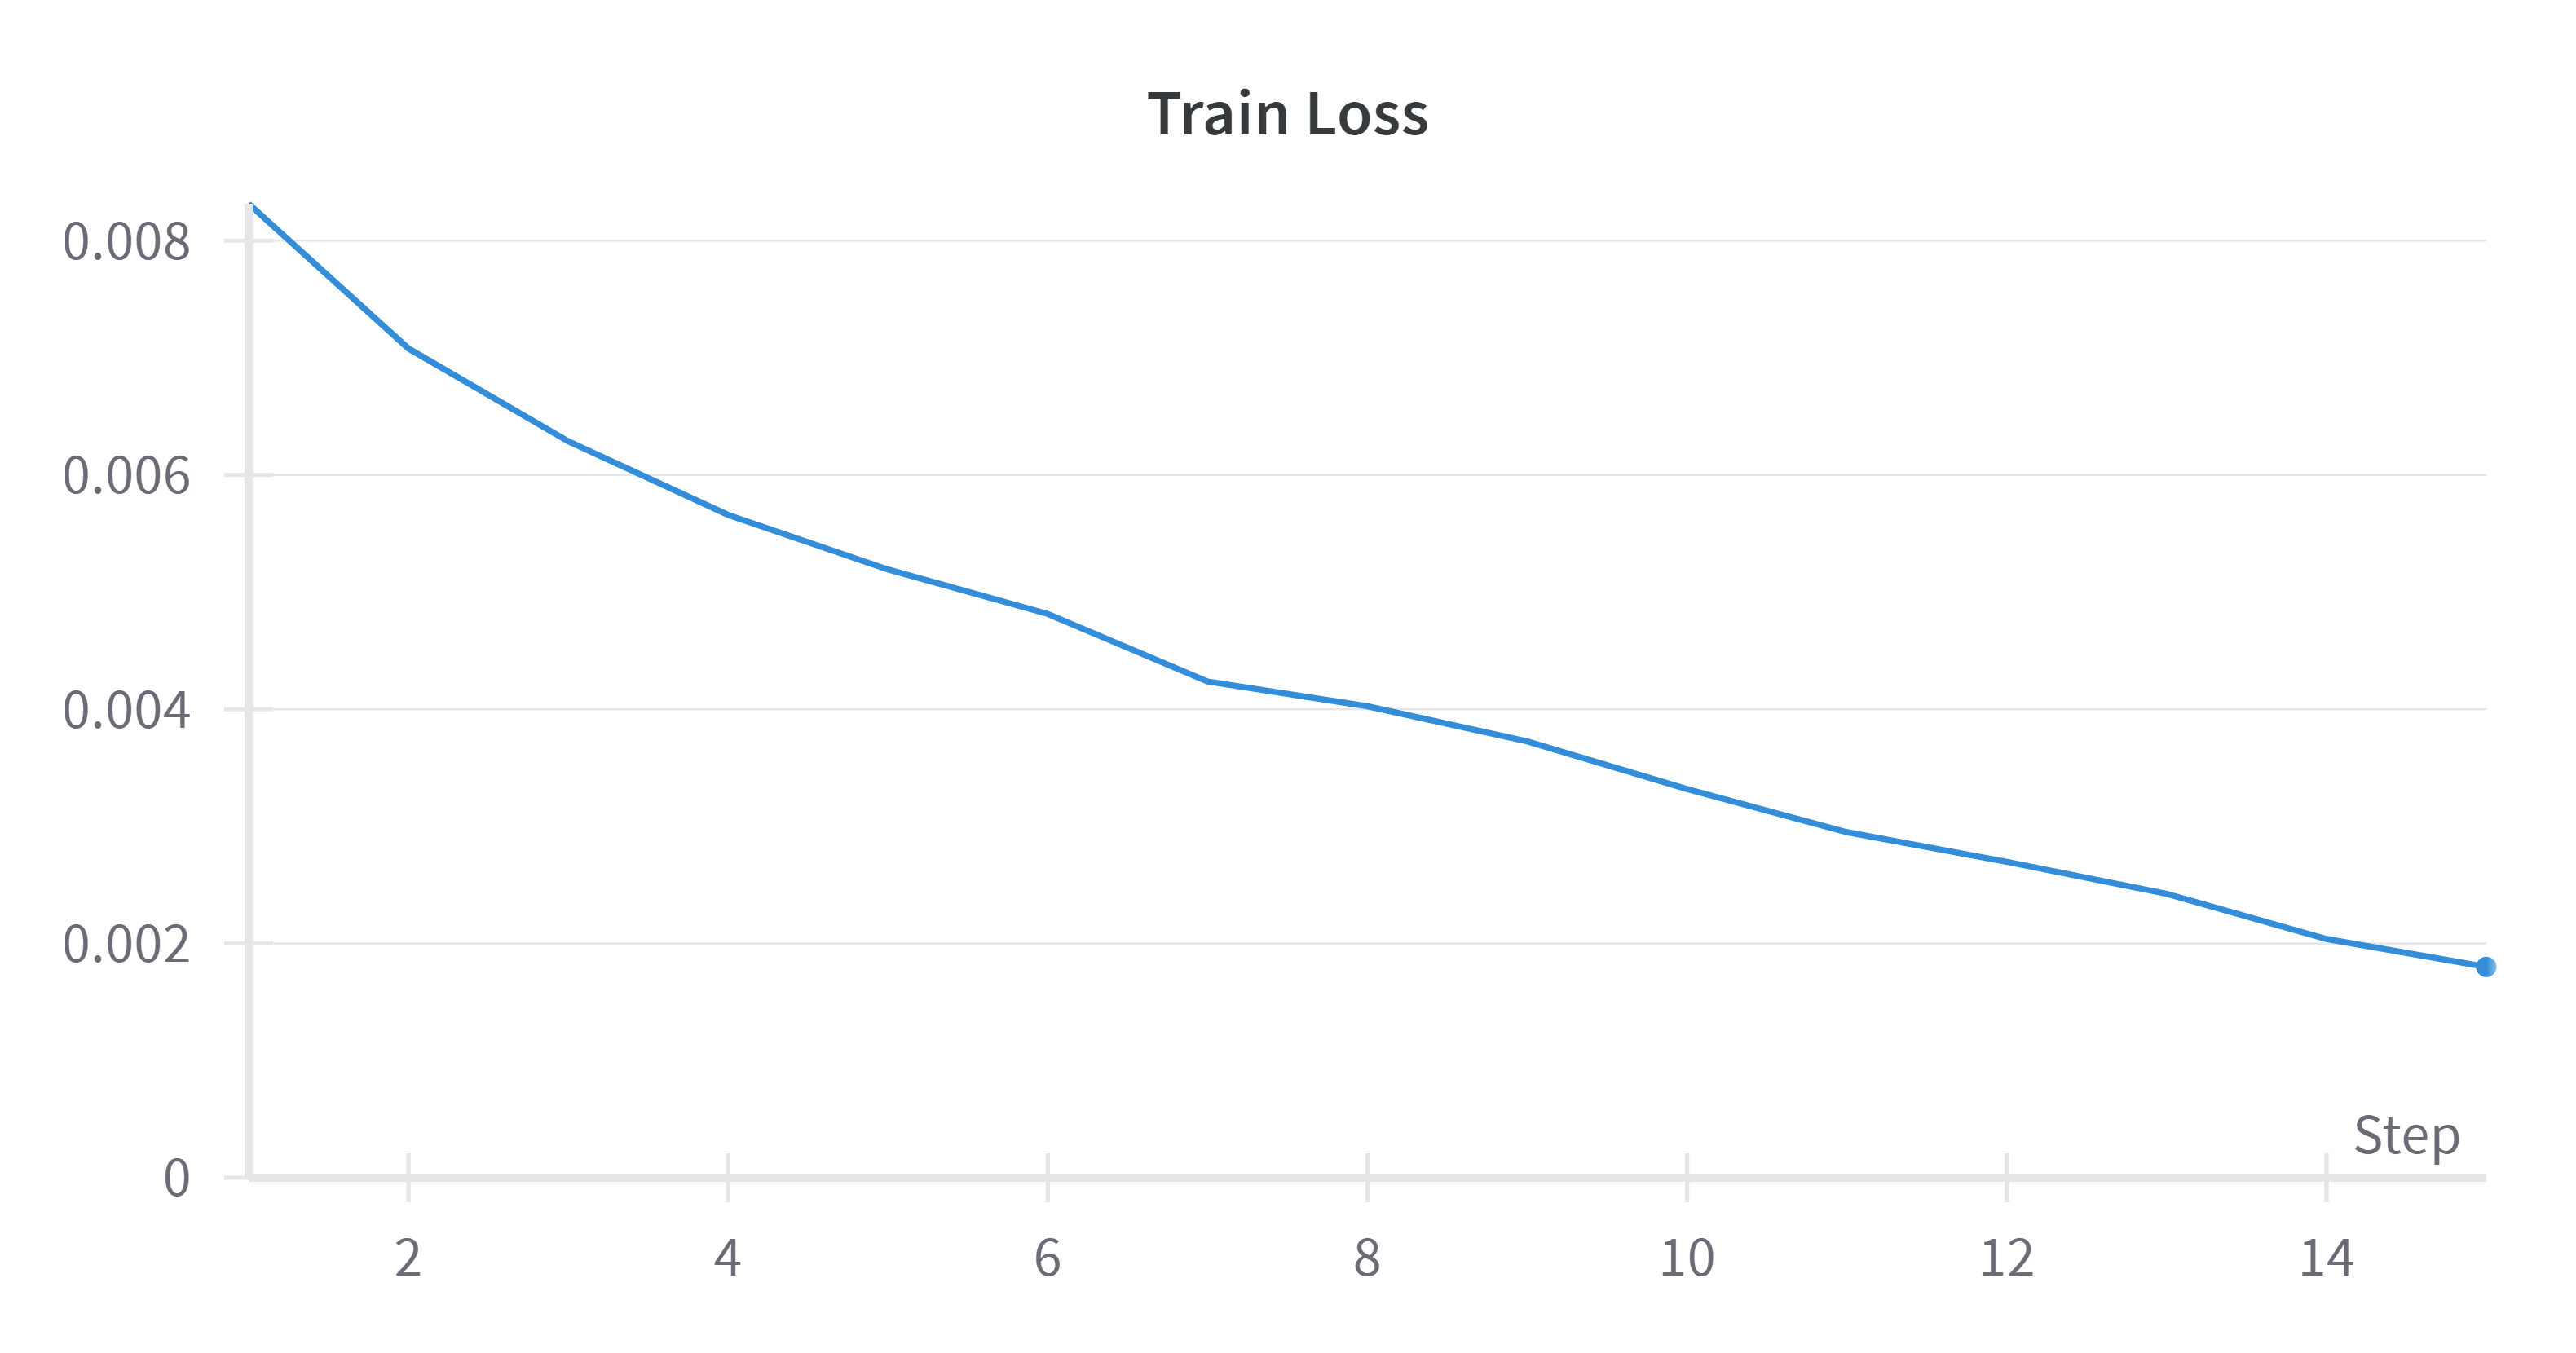
\includegraphics[width=0.4\textwidth]{Assets/Classification/Convnet/01}
            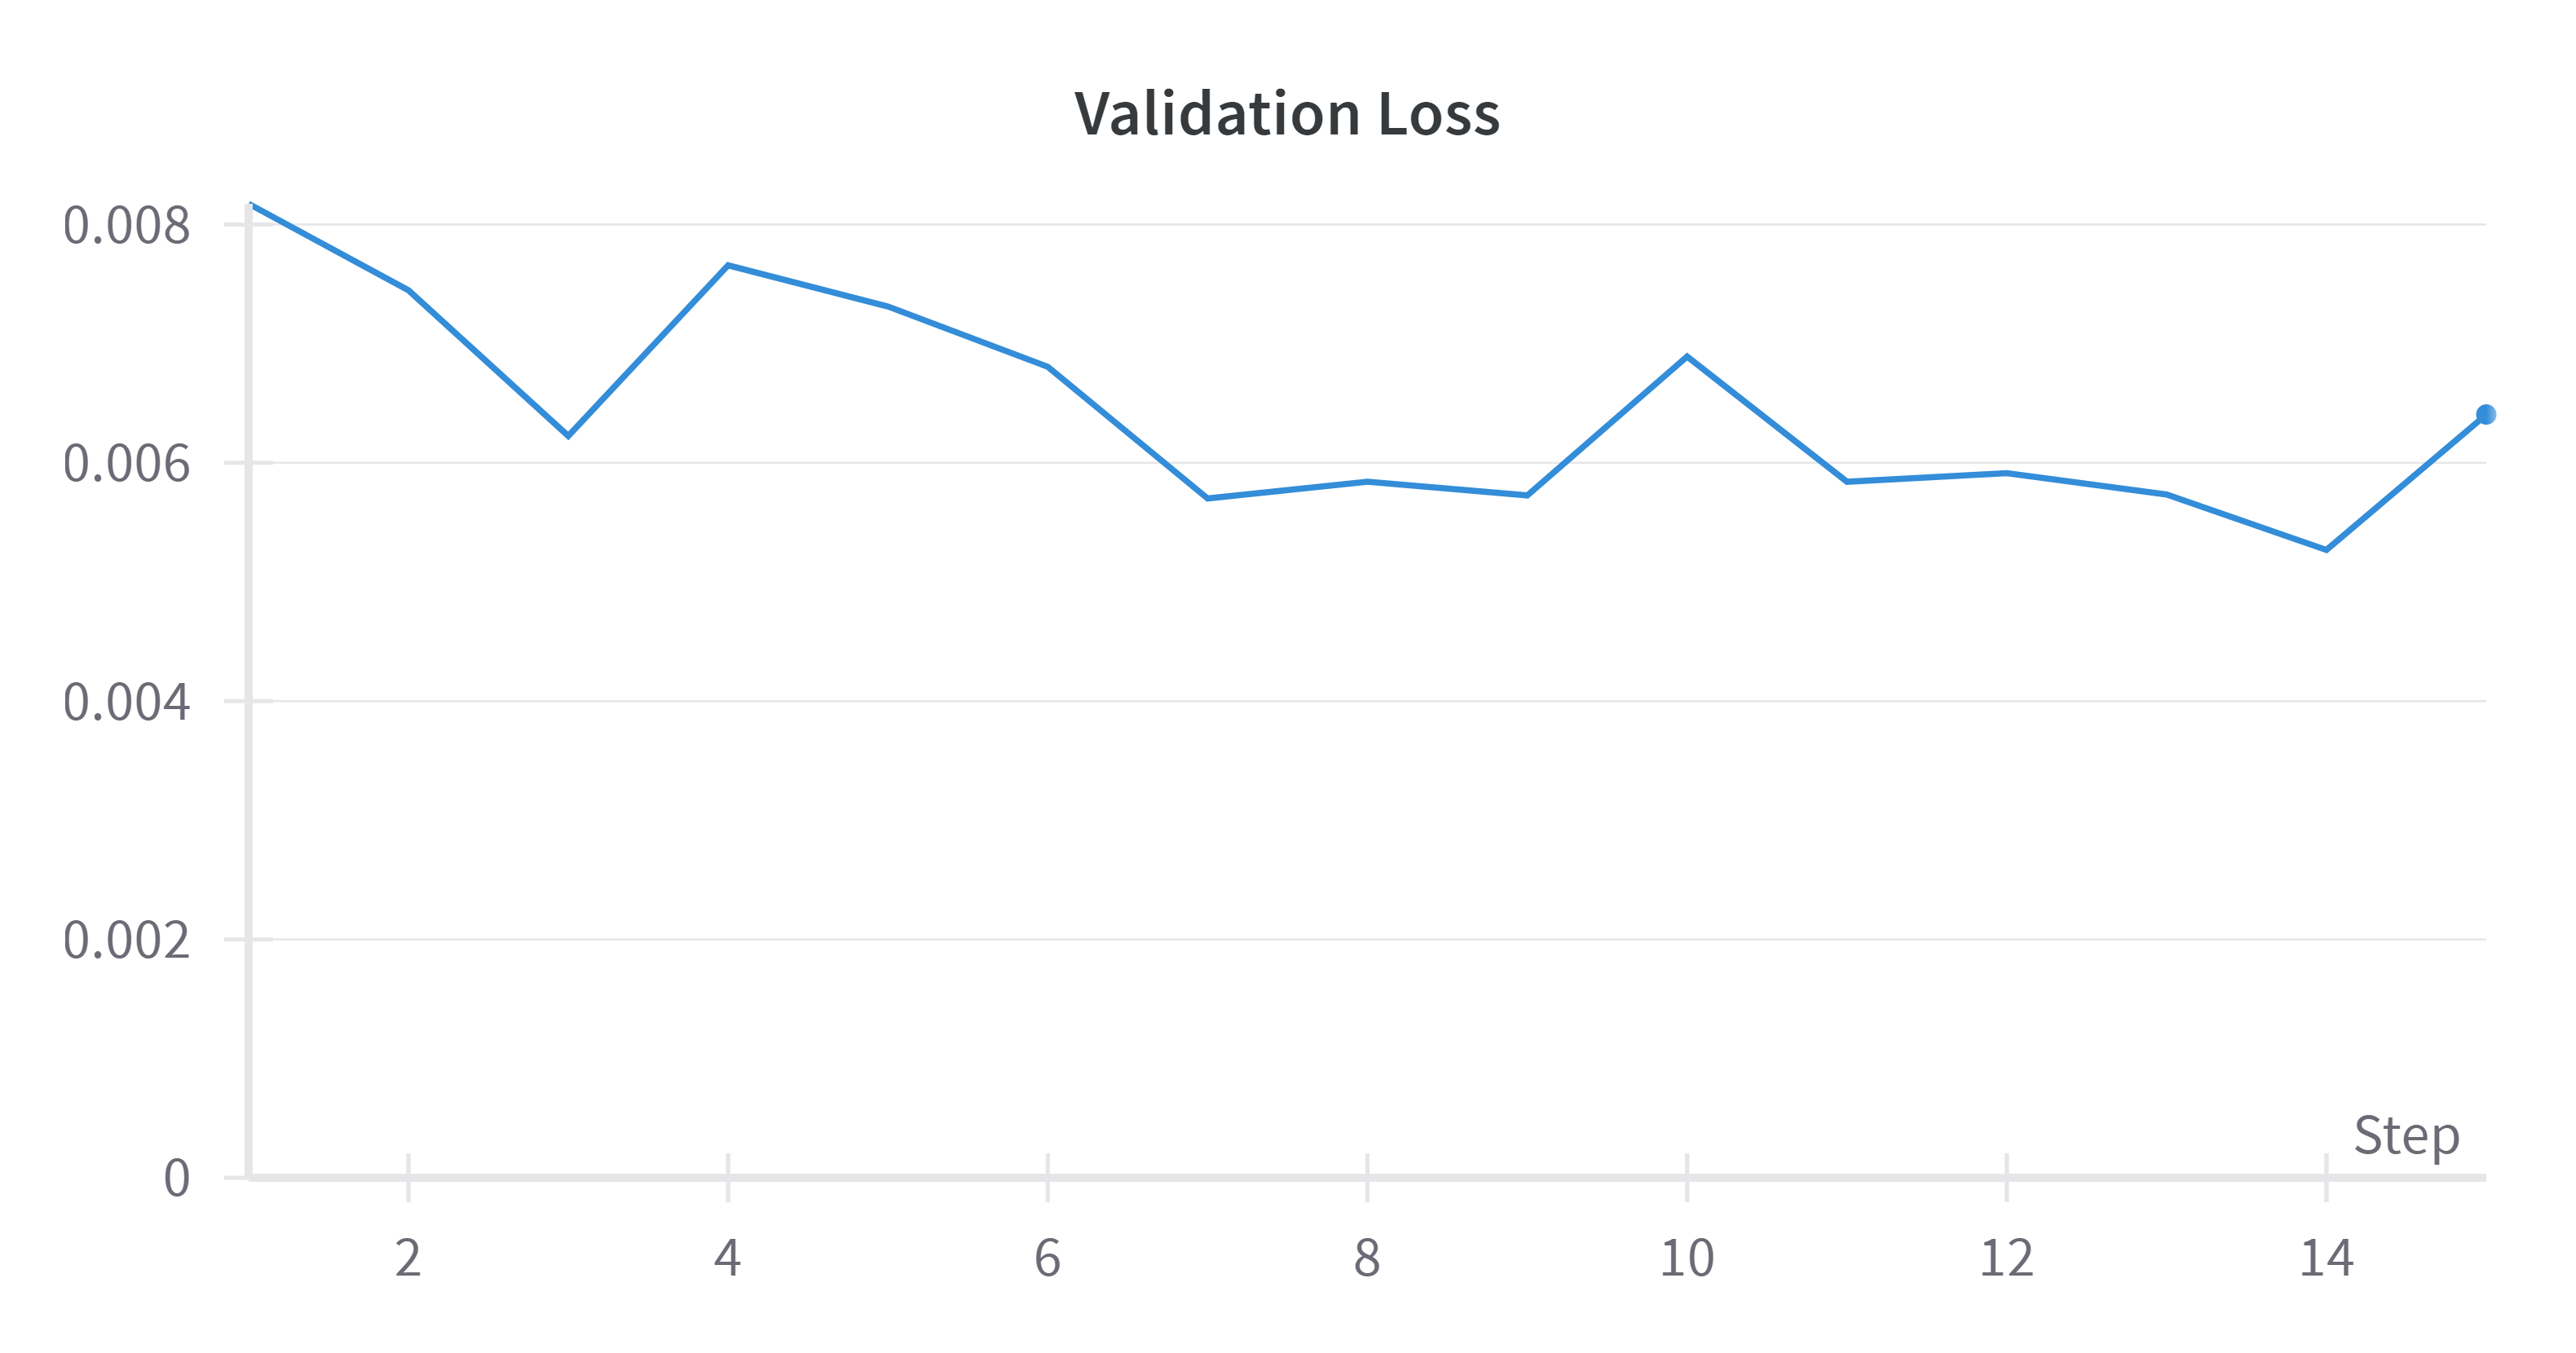
\includegraphics[width=0.4\textwidth]{Assets/Classification/Convnet/02}
            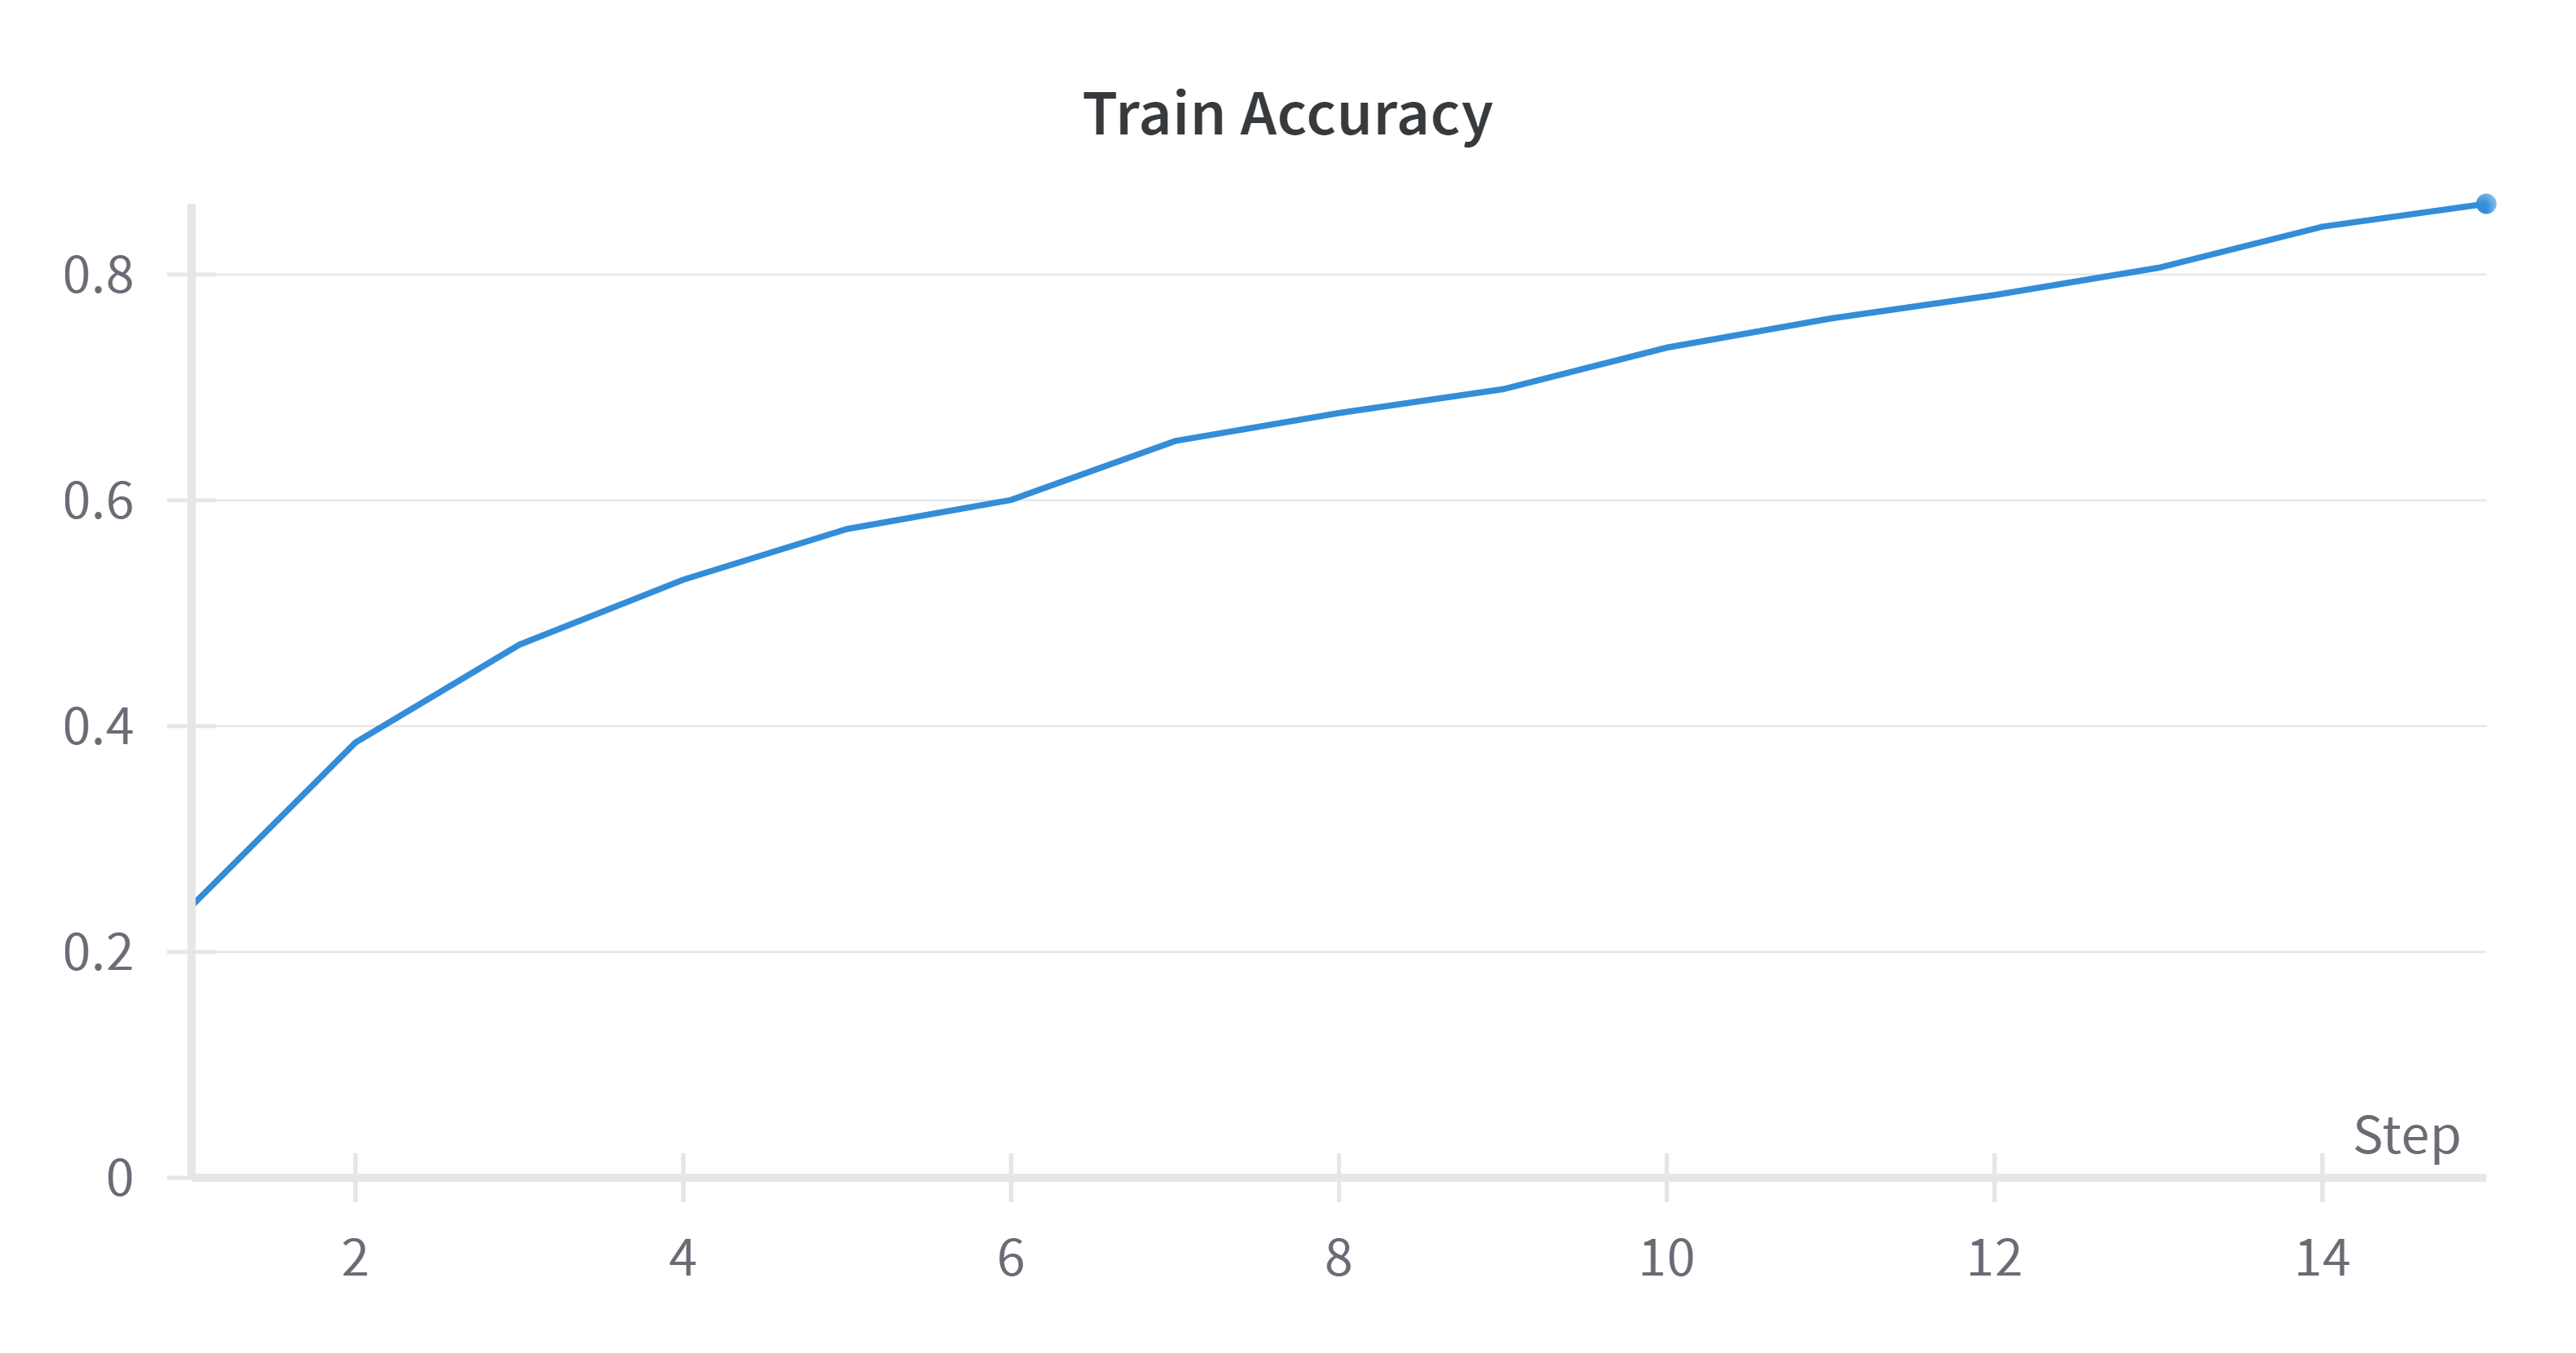
\includegraphics[width=0.4\textwidth]{Assets/Classification/Convnet/03}
            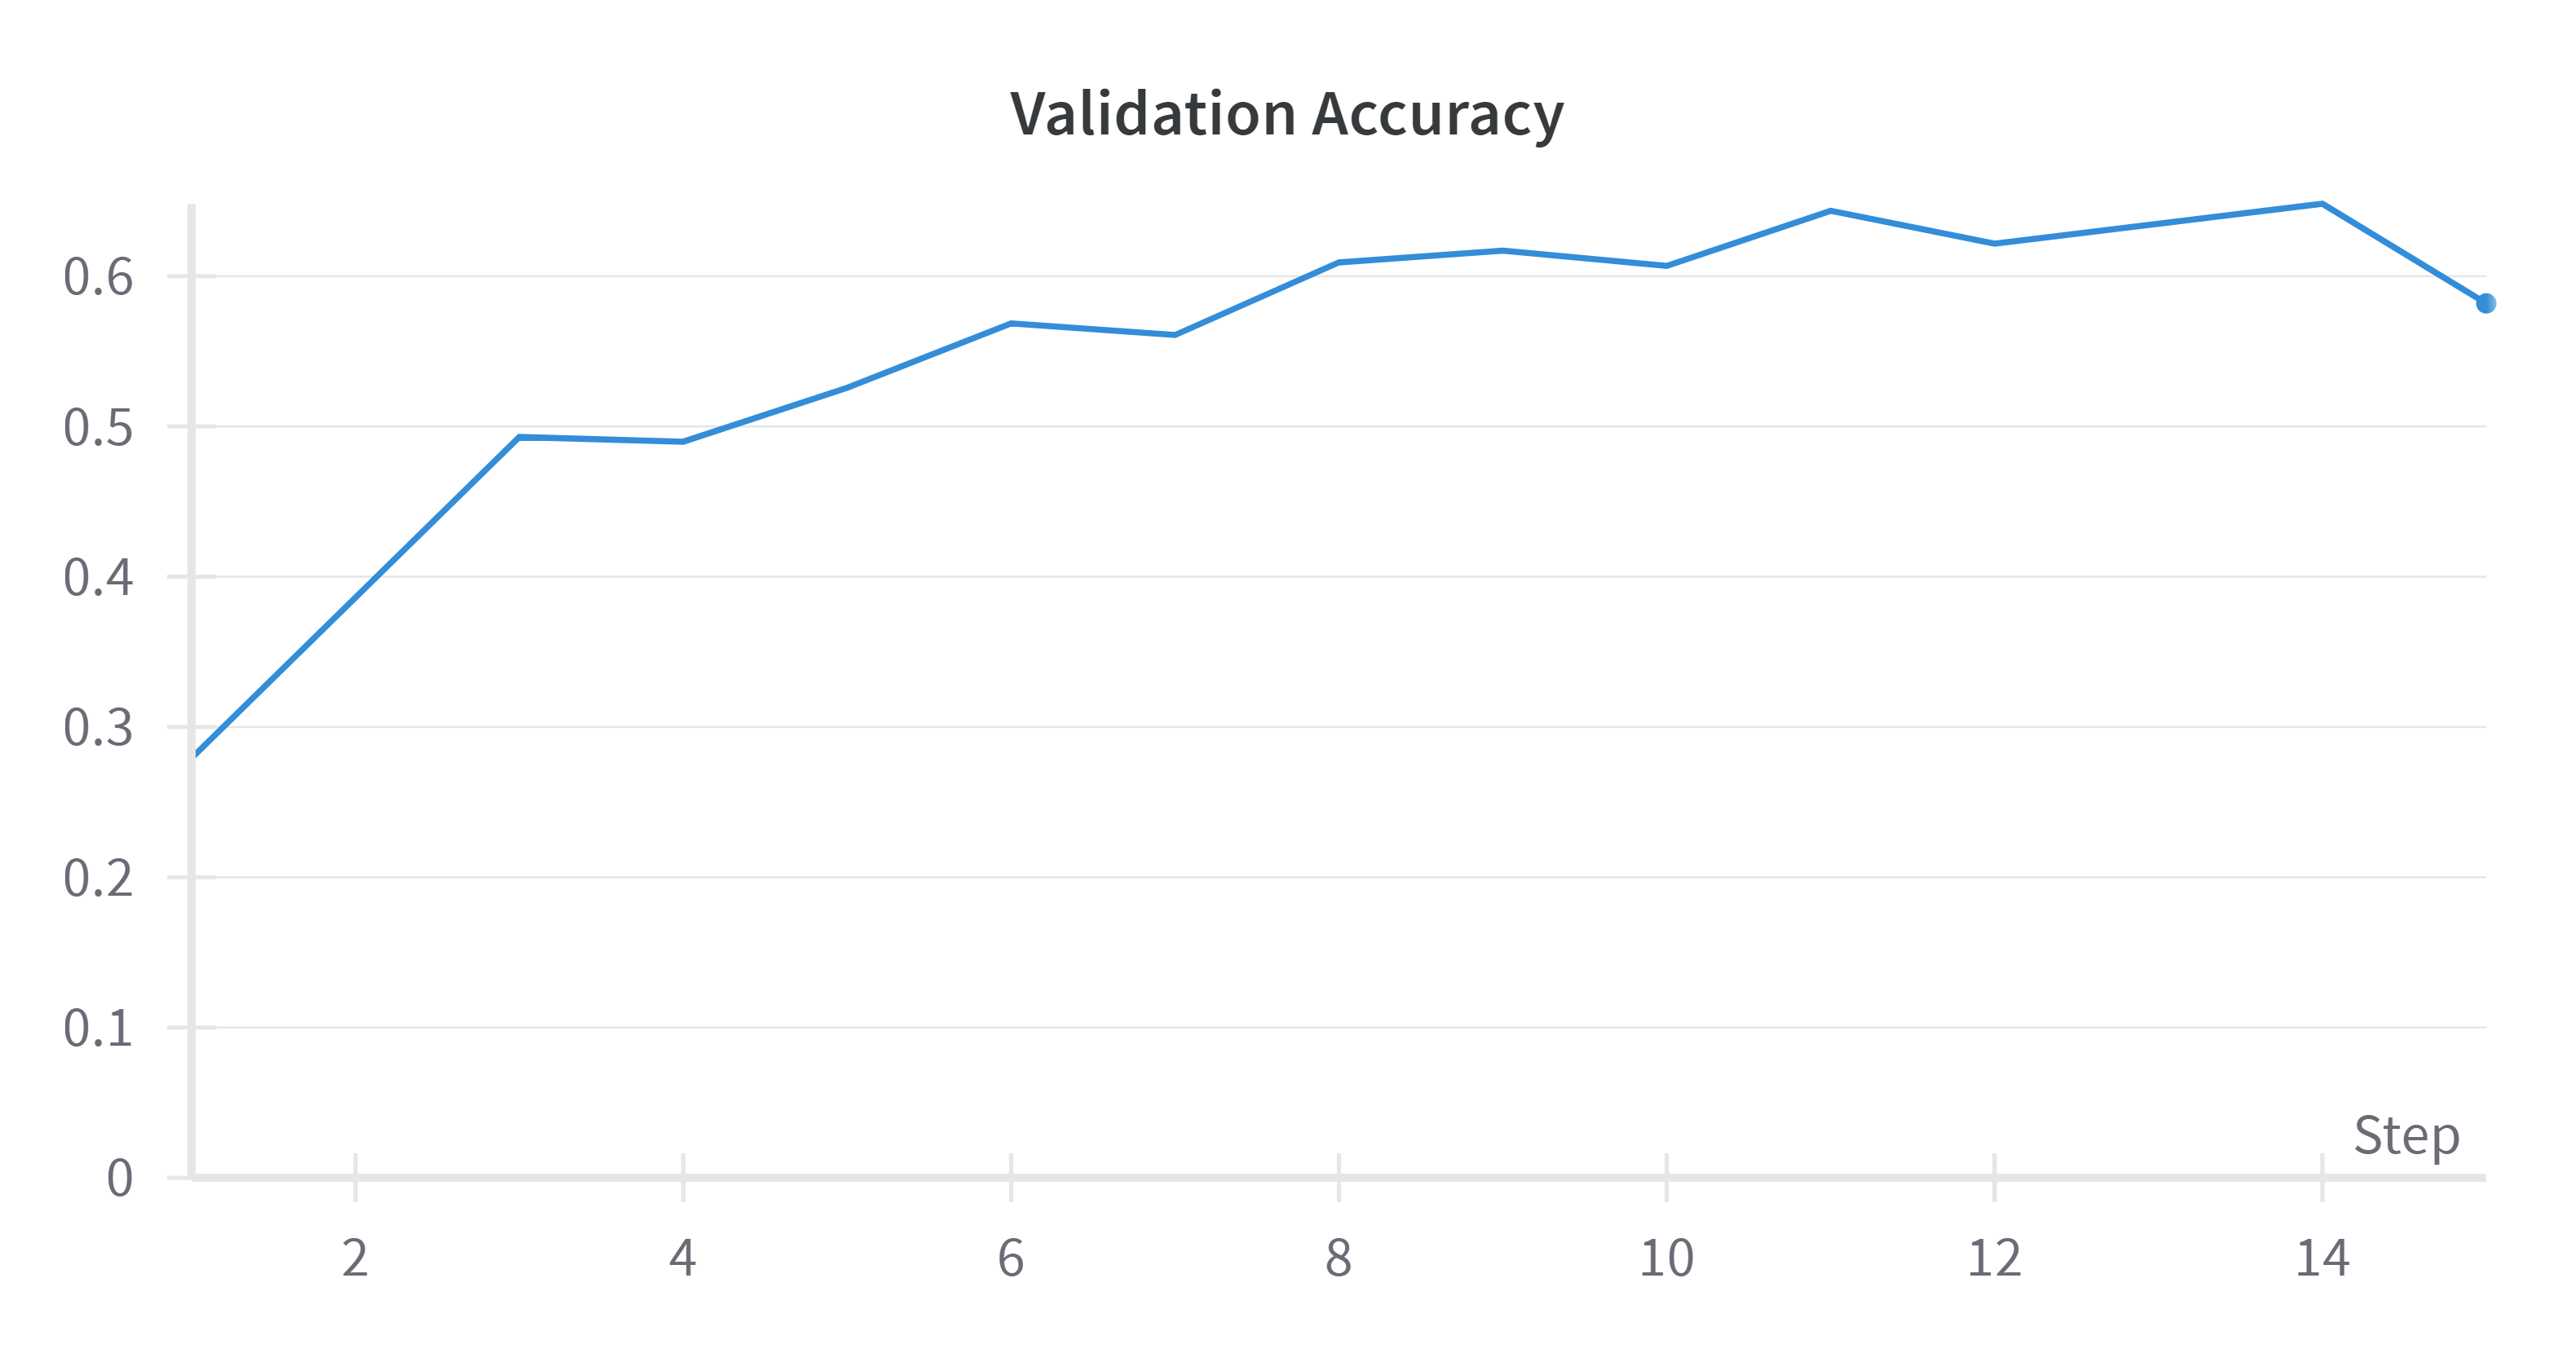
\includegraphics[width=0.4\textwidth]{Assets/Classification/Convnet/04}
            \caption{Loss and Accuracy curves (per epoch) for the given CNN architecture}
            \label{fig:convnet-loss-accuracy-curves}
        \end{figure}
        \item Looking at the figures, it is clear that the model is overfitting after
        training for a few epochs, since the validation loss stops decreasing sharply
        while the training loss keeps decreasing. There is a large gap between the training
        and validation losses, and the same goes for accuracies. The final training accuracy
        after 15 epochs is close to 0.86+, while the validation accuracy was around 0.58+ only.
        \item The confusion matrix (logged using wandb) is given in Figure (\ref{fig:convnet-conf-matrix}).
        However, it is still surprisig that the accuracy on the test set was 0.917+. This
        is a good example of why accuracy is not the only indicator of a model's performance.
        The precision, recall, and F1-score for the classification all turned out to be 0.588+.
        \begin{figure}[h!]
            \centering
            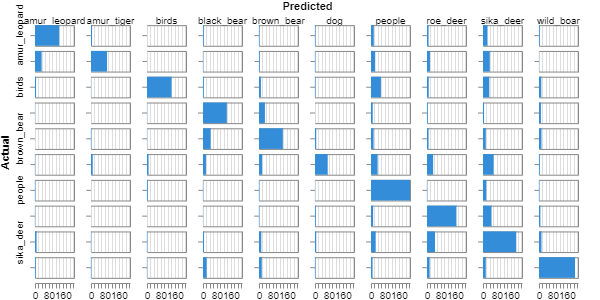
\includegraphics[width=0.7\textwidth]{Assets/Classification/Convnet/05}
            \caption{Confusion Matrix for the given CNN architecture}
            \label{fig:convnet-conf-matrix}
        \end{figure}
        \item Finally, we visualize 3 misclassified images from each class. These are also
        given in the same notebook. A few examples are also given in Figure
        (\ref{fig:convnet-misclassifications}). There were quite a few examples where the
        ground truth class was not present or did not cover a majority of the image. For
        example, some images of class \texttt{amur\_leopard} were not clear. In some cases,
        the ground truth class was also not present, for example, in case of \texttt{black\_bear}.
        There was also a case where the image looks like the predicted class - \texttt{brown\_bear}
        being predicted as \texttt{black\_bear} and \texttt{wild\_bear}.
        \begin{figure}[h!]
            \centering
            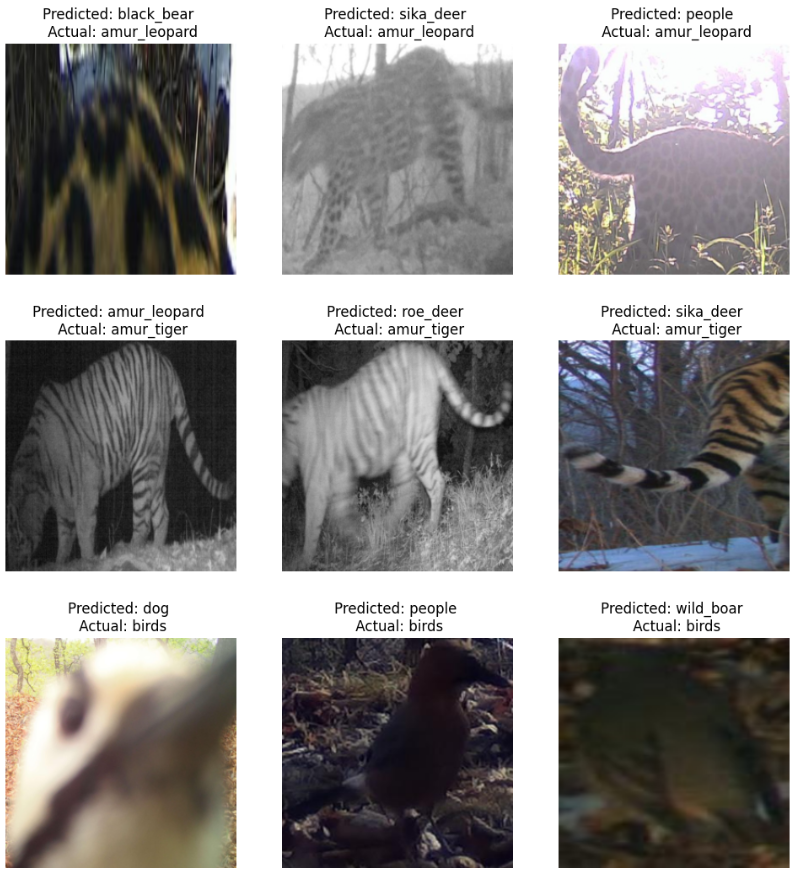
\includegraphics[width=0.325\textwidth]{Assets/Classification/Convnet/Misclassifications/01}
            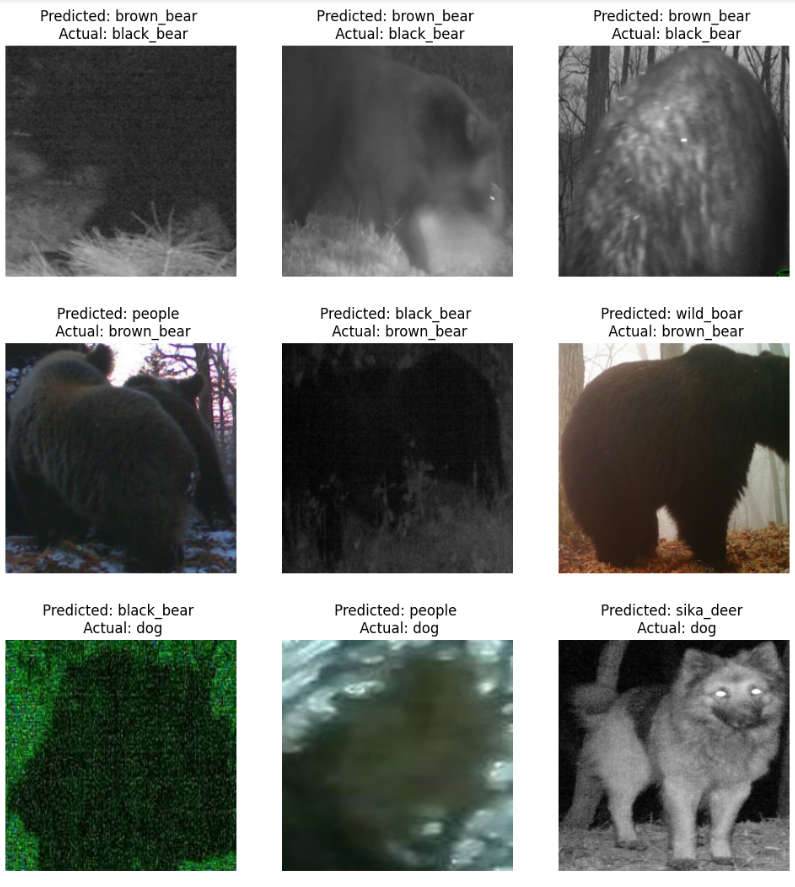
\includegraphics[width=0.325\textwidth]{Assets/Classification/Convnet/Misclassifications/02}
            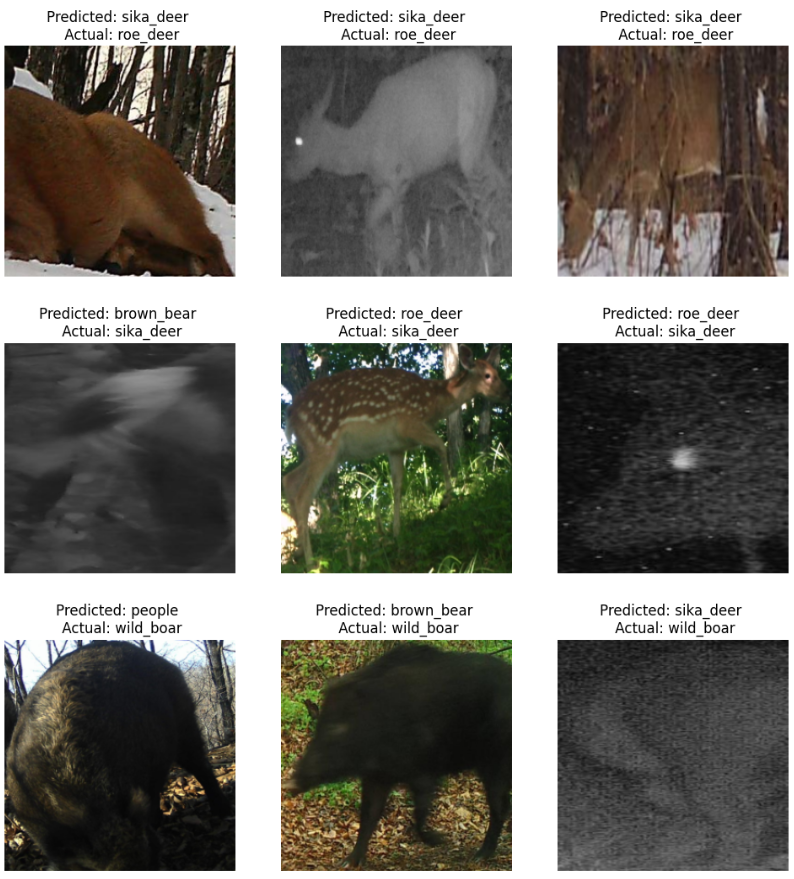
\includegraphics[width=0.325\textwidth]{Assets/Classification/Convnet/Misclassifications/03}
            \caption{Classwise examples of misclassified images}
            \label{fig:convnet-misclassifications}
        \end{figure}
    \end{enumerate}

    \subsection*{\textbf{Question 3.}}
    \begin{enumerate}[label=(\alph*)]
        \item Next, we finetune the Resnet-18 model availble in PyTorch on the Russian Wildlife
        dataset. The model was finetuned for a total of 10 epochs due to computational limitations.
        The per epoch loss/accuracy curves generated using wandb are given in Figure
        (\ref{fig:resnet-loss-accuracy-curves}).
        \begin{figure}[h!]
            \centering
            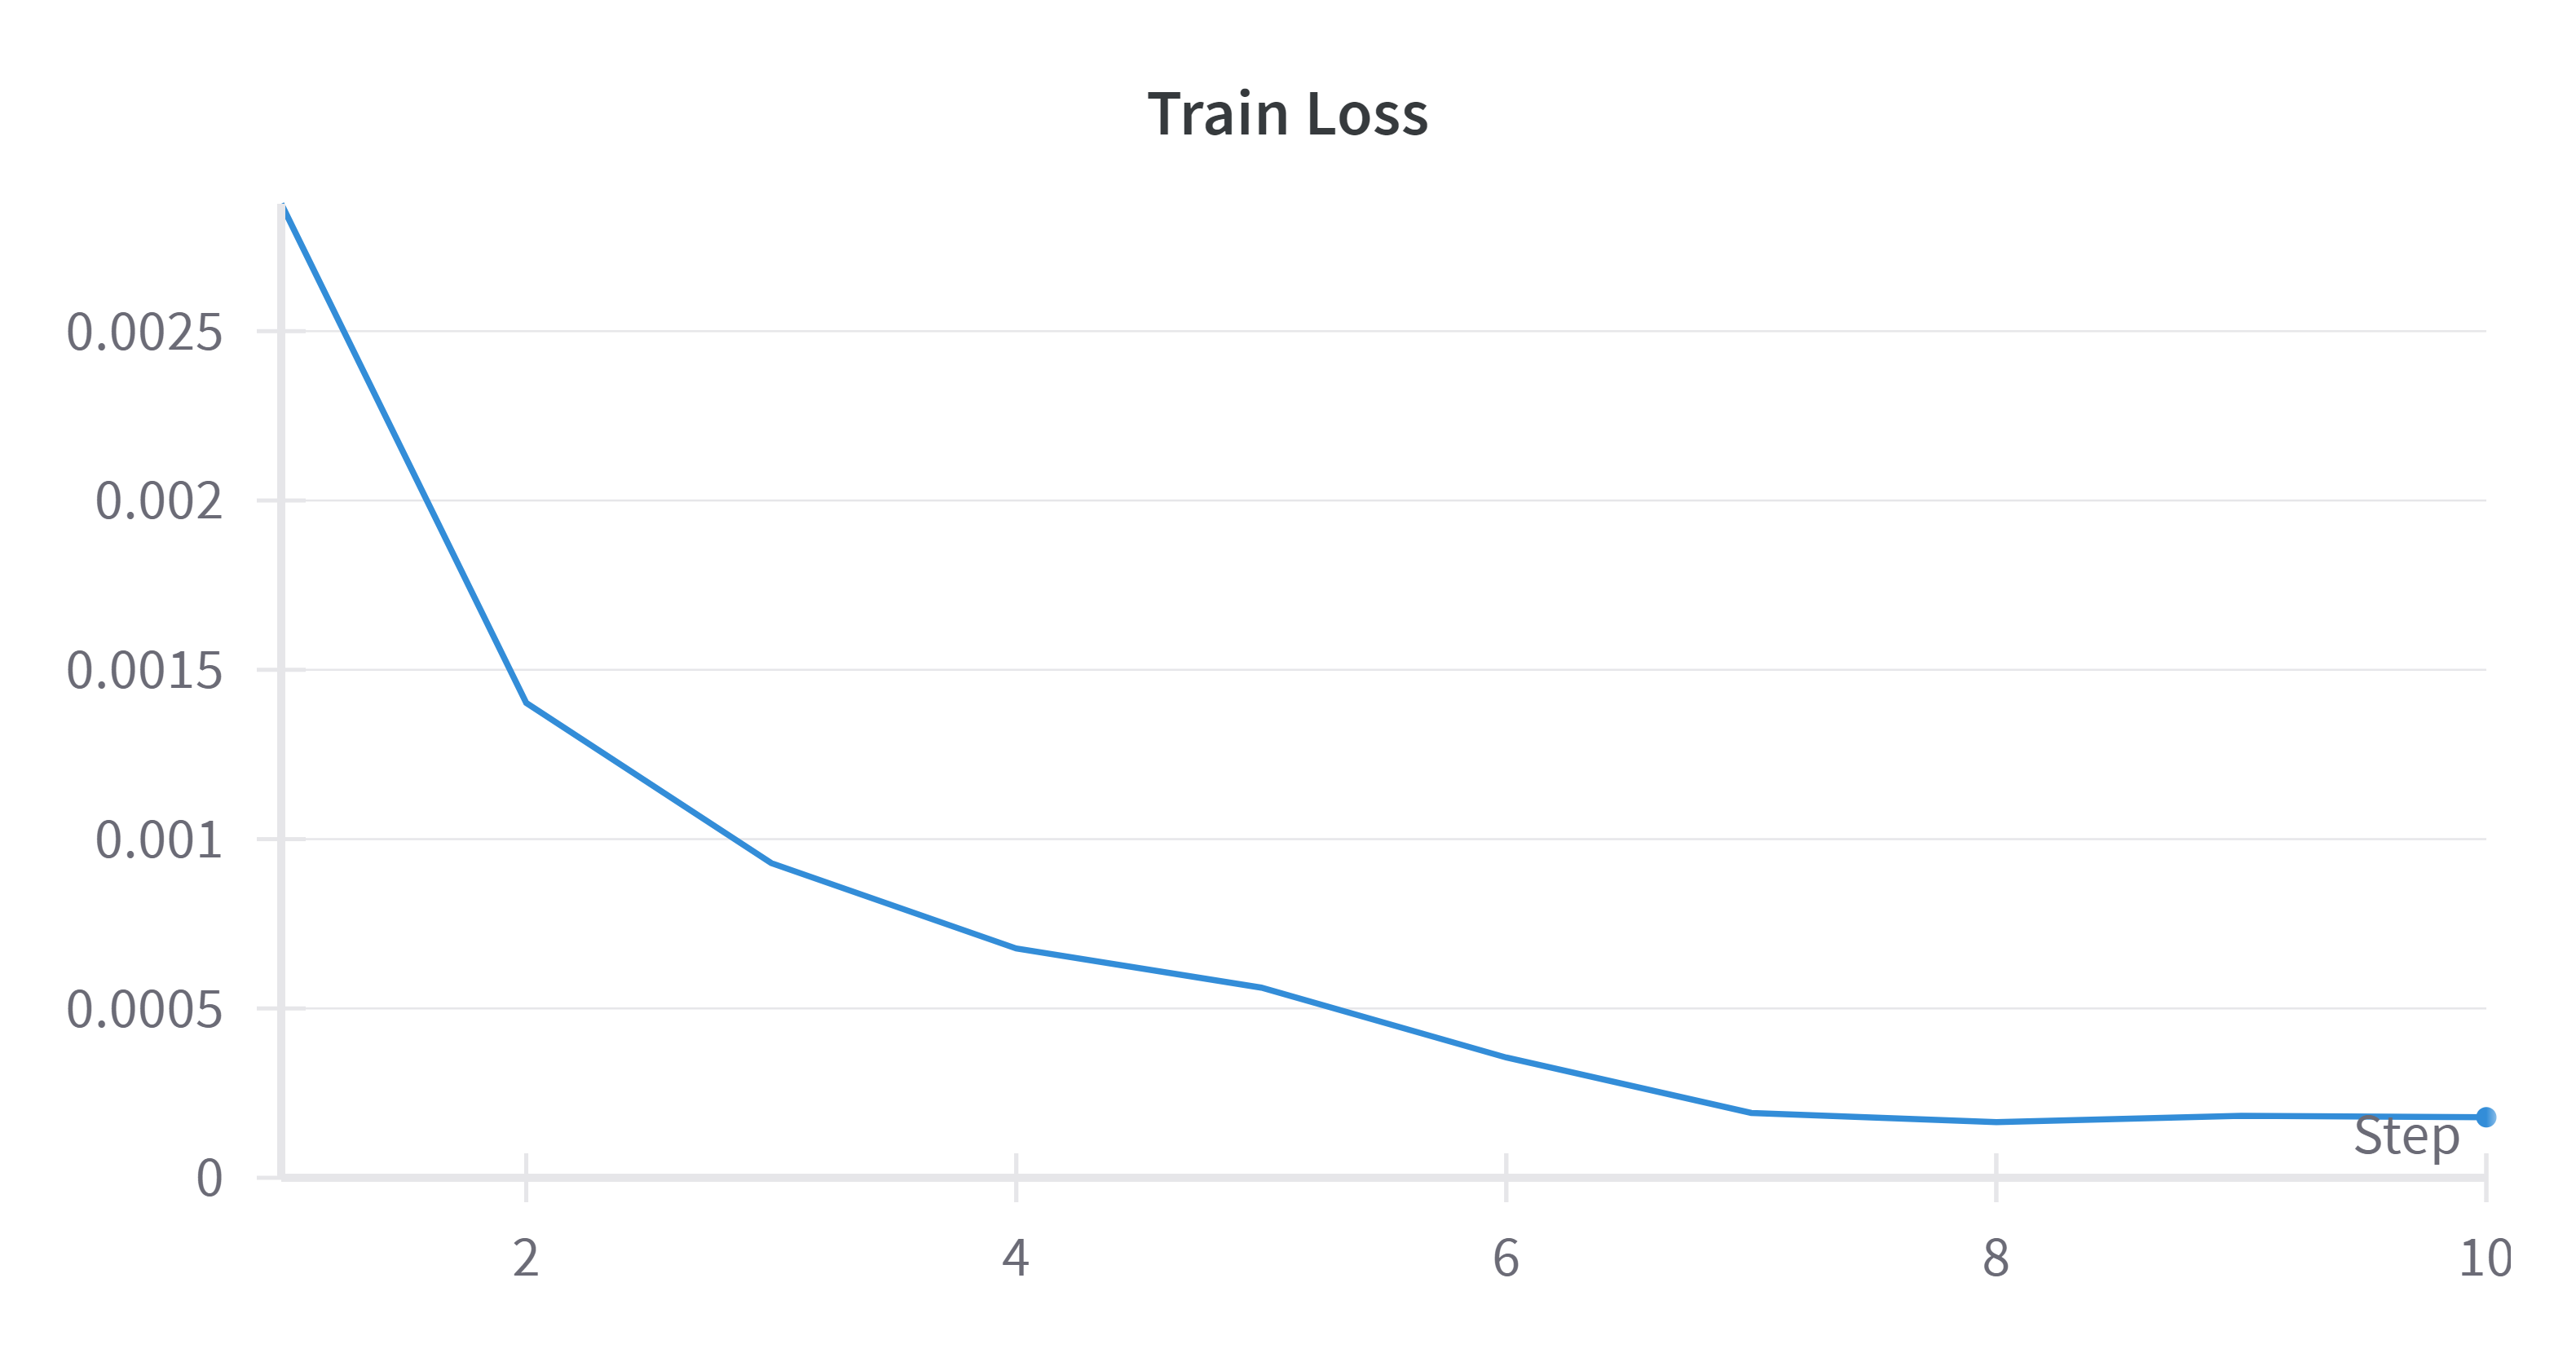
\includegraphics[width=0.4\textwidth]{Assets/Classification/Resnet/01}
            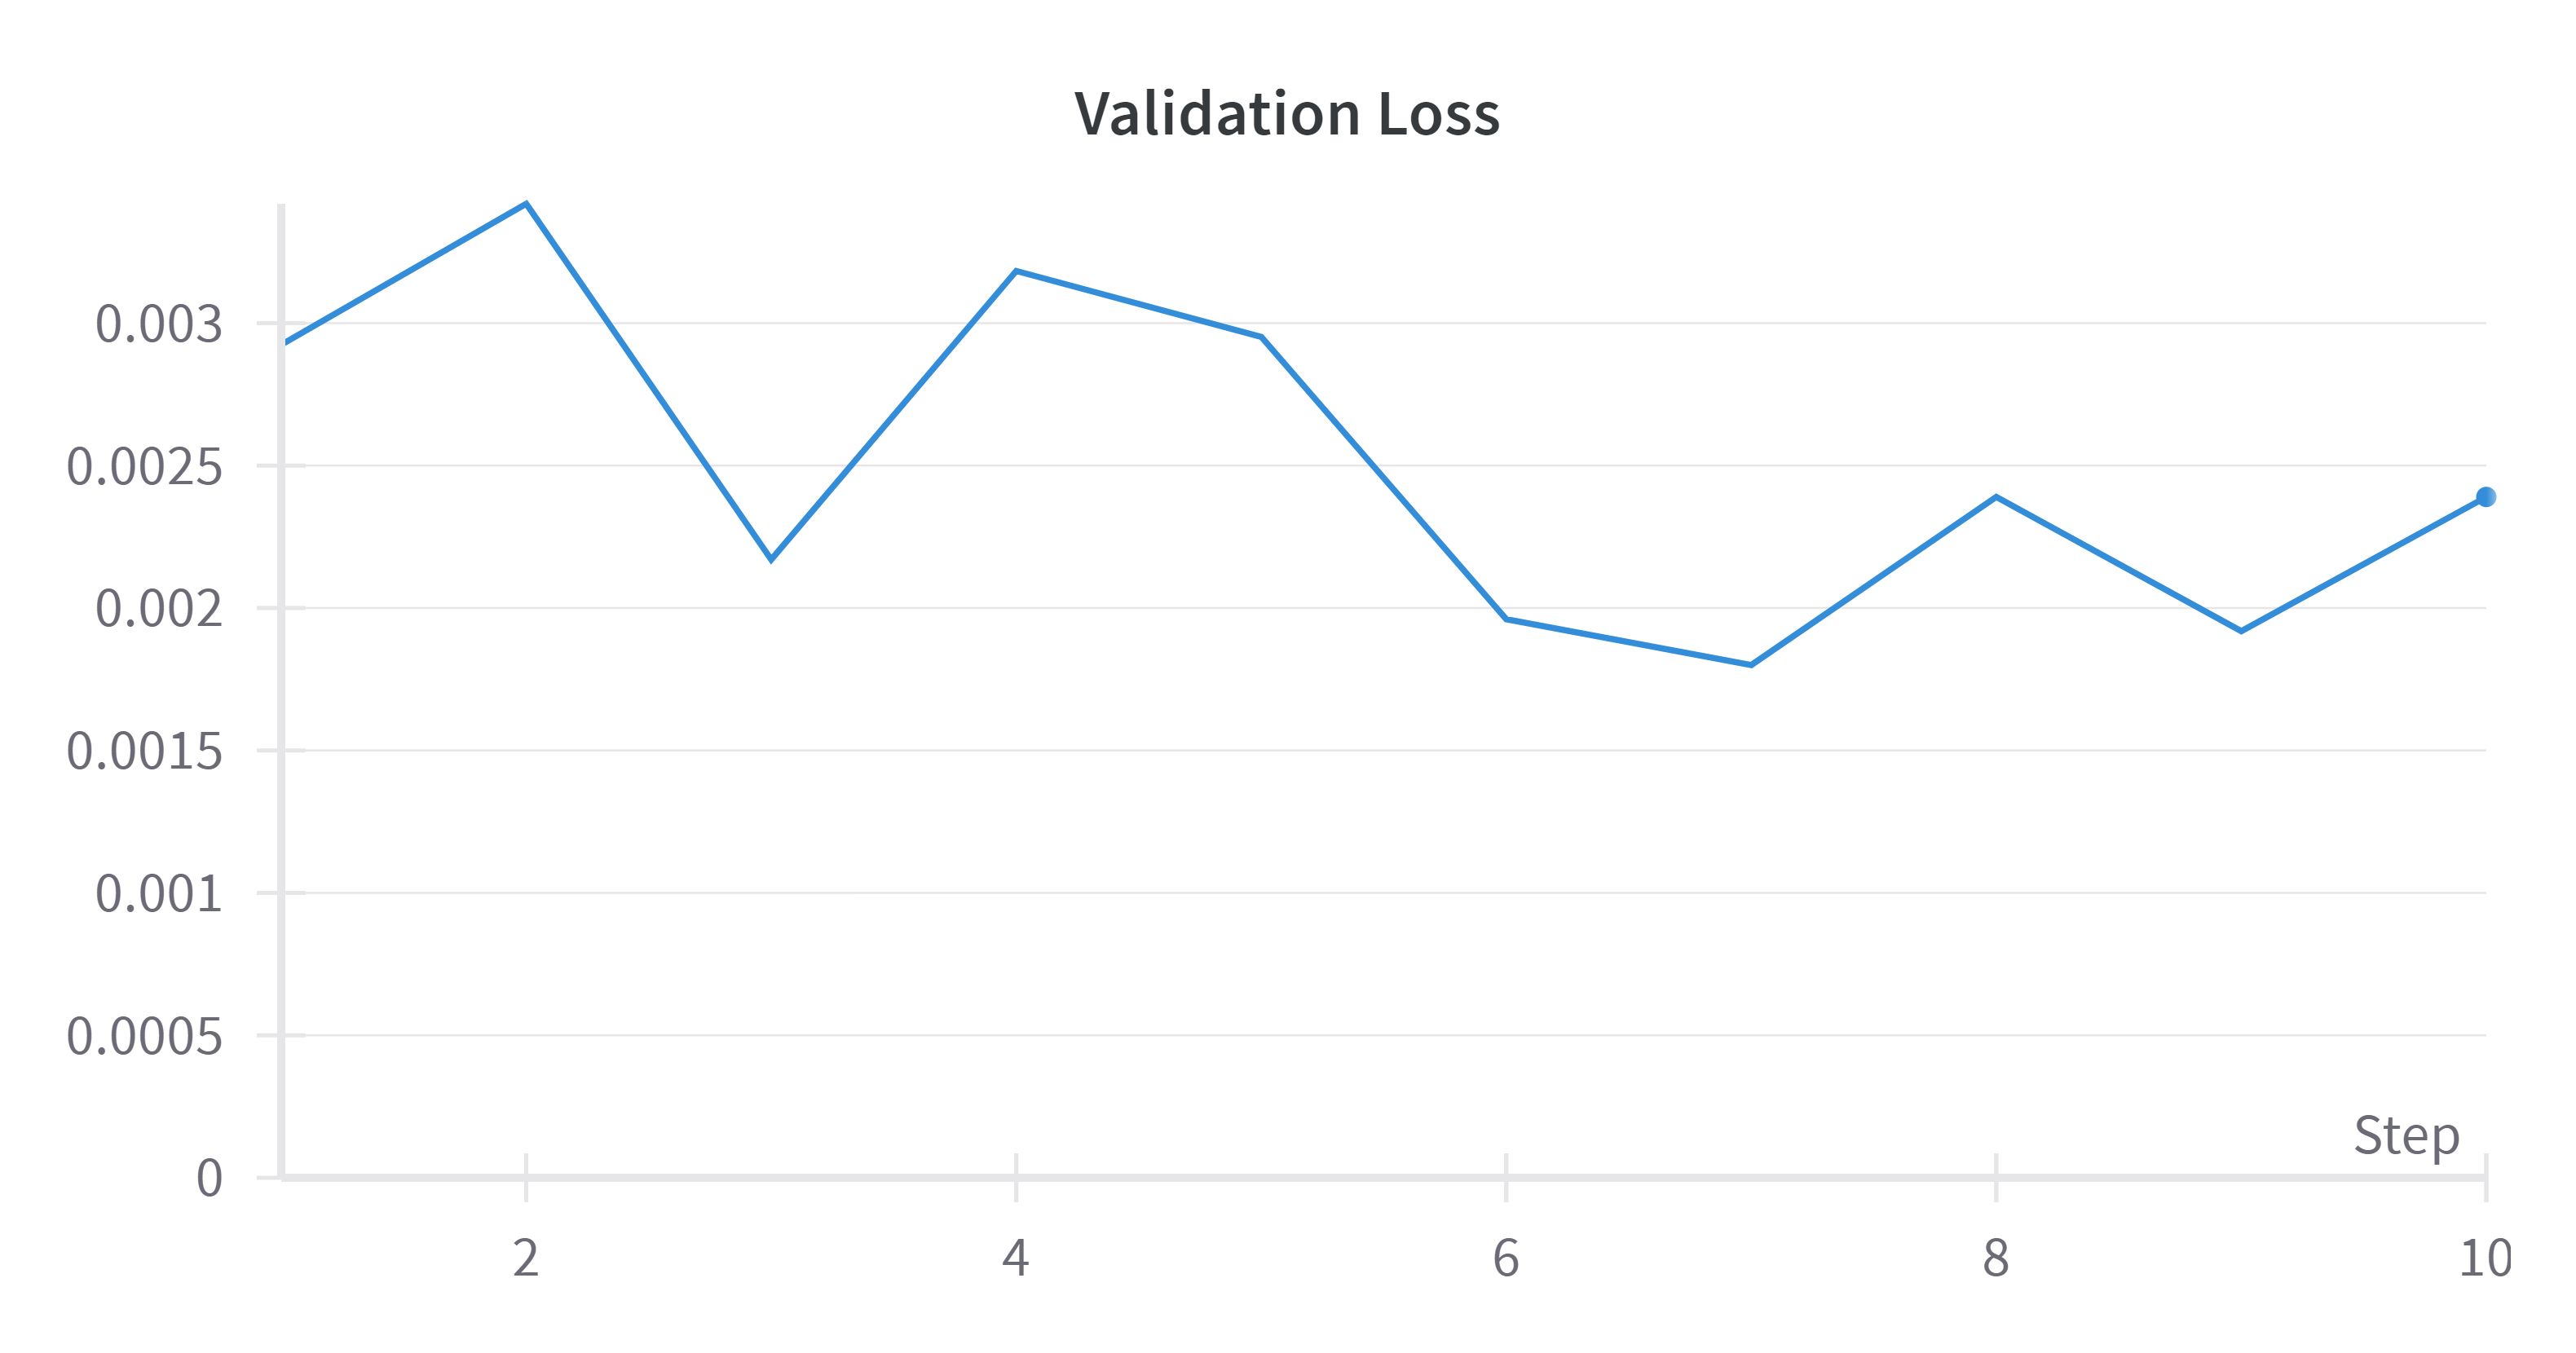
\includegraphics[width=0.4\textwidth]{Assets/Classification/Resnet/02}
            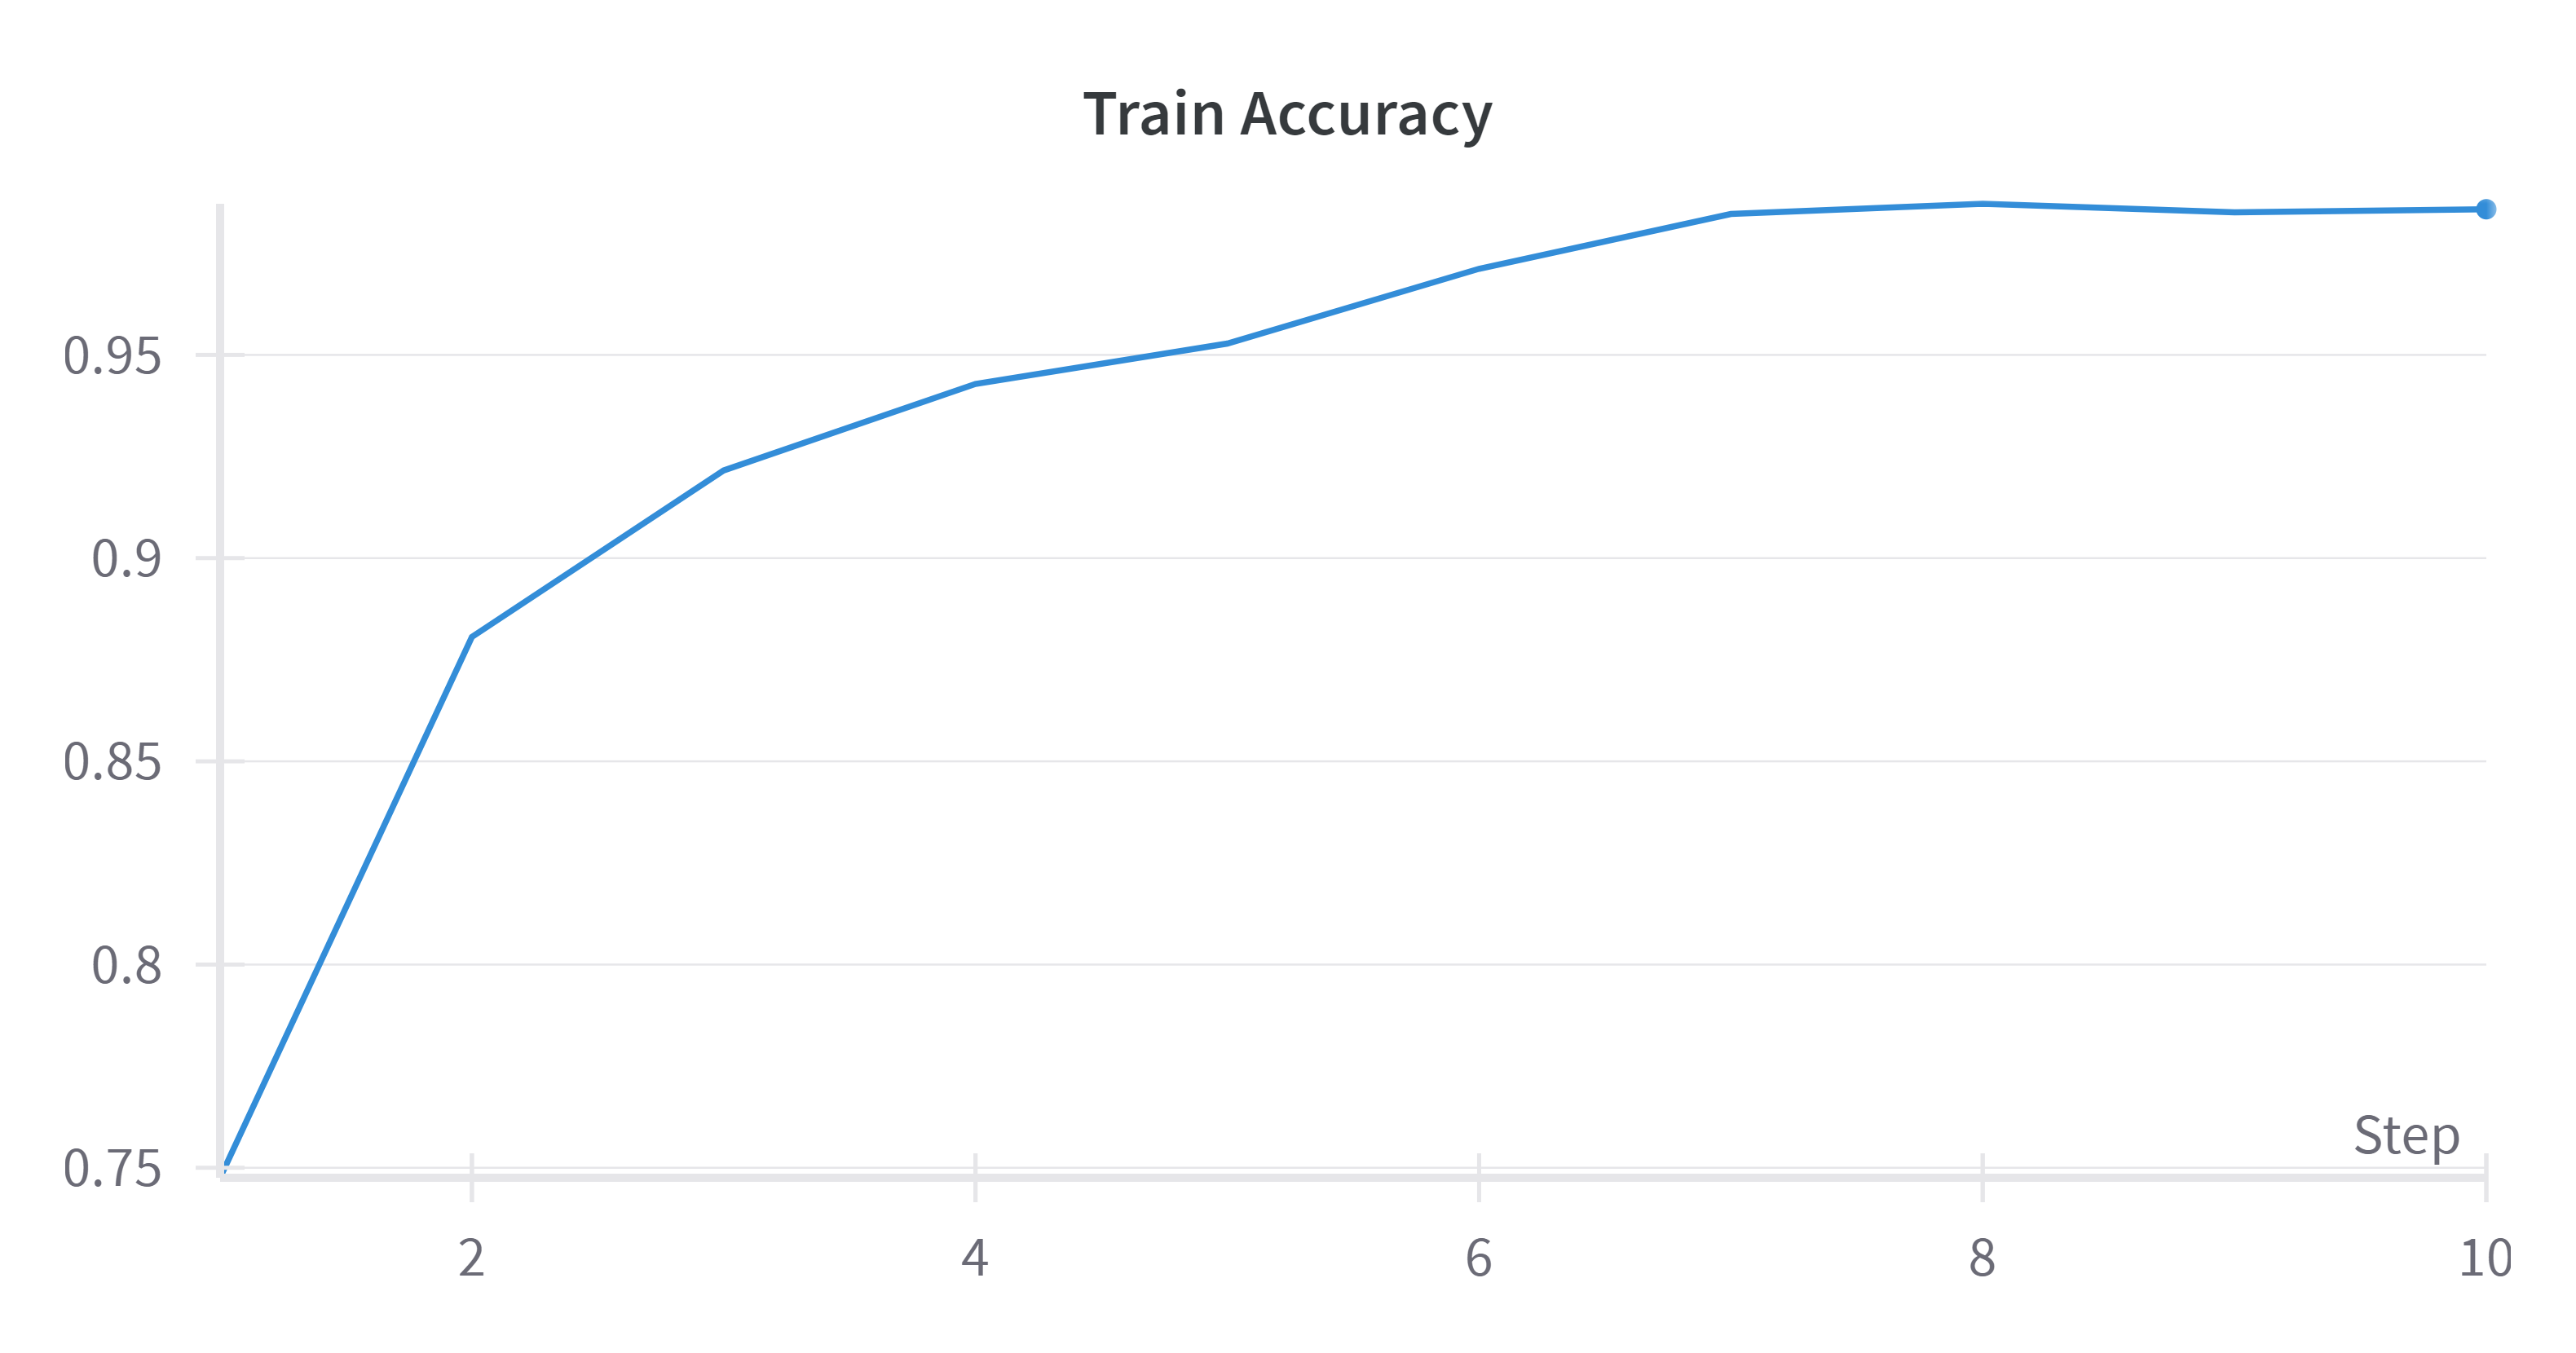
\includegraphics[width=0.4\textwidth]{Assets/Classification/Resnet/03}
            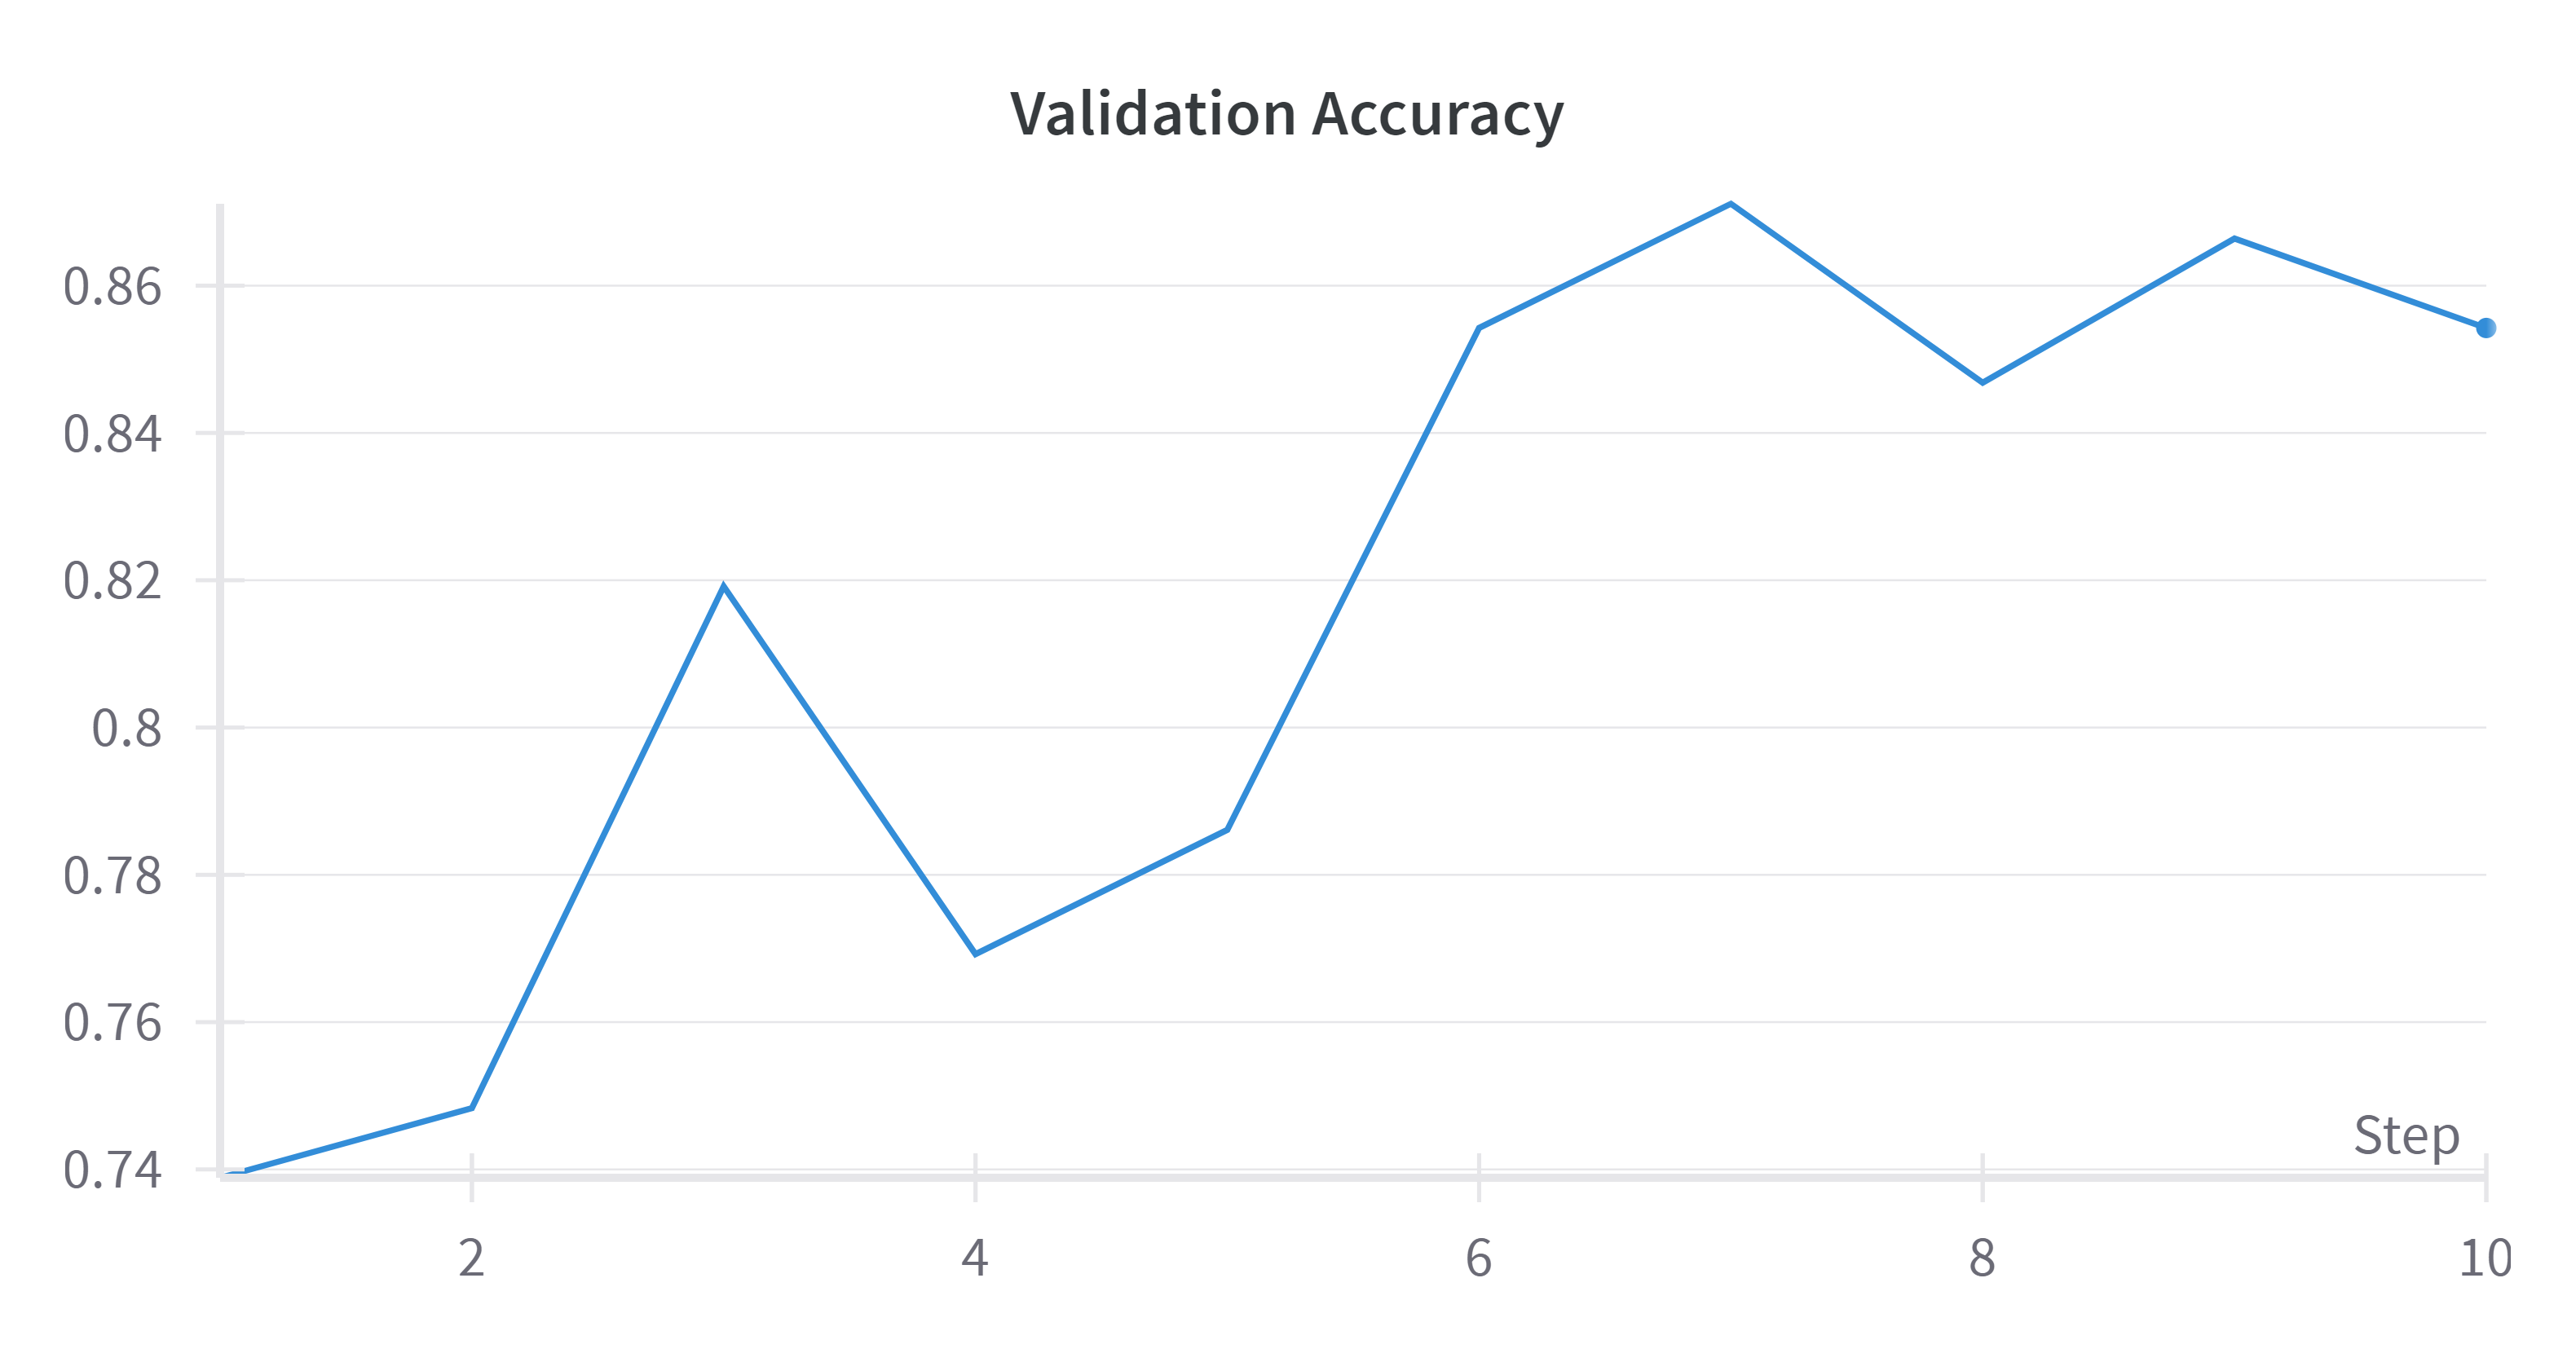
\includegraphics[width=0.4\textwidth]{Assets/Classification/Resnet/04}
            \caption{Loss and Accuracy curves (per epoch) for Resnet-18}
            \label{fig:resnet-loss-accuracy-curves}
        \end{figure}
        \item This model is not overfitting as much as the previous model. This is
        inferred because the difference between the training loss and validation loss
        is lower, and the same goes for the accuracy.
        \item The Resnet-18 mmodel performed better than the previous model. It achieved
        an accuracy of 0.969+. The precision, recall, and F1-score for the classification
        all turned out to be 0.846+. The confusion matrix (logged using wandb) is given in
        Figure (\ref{fig:resnet-conf-matrix}).
        \begin{figure}[h!]
            \centering
            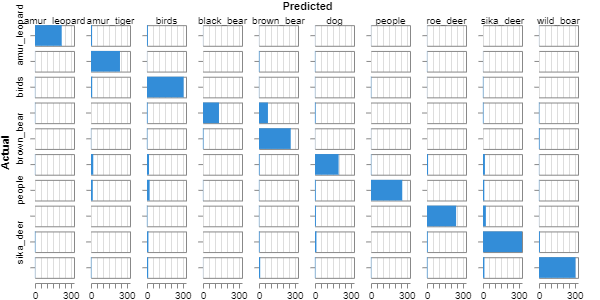
\includegraphics[width=0.7\textwidth]{Assets/Classification/Resnet/05}
            \caption{Confusion Matrix for the Resnet-18 architecture}
            \label{fig:resnet-conf-matrix}
        \end{figure}
        \item The 2D and 3D representations of the feature space generated by input samples
        from training and validation sets by the classifier were generated and are given in
        Figure (\ref{fig:resnet-tsne-2d}) and Figure (\ref{fig:resnet-tsne-3d}) respectively.
        \begin{figure}[h!]
            \centering
            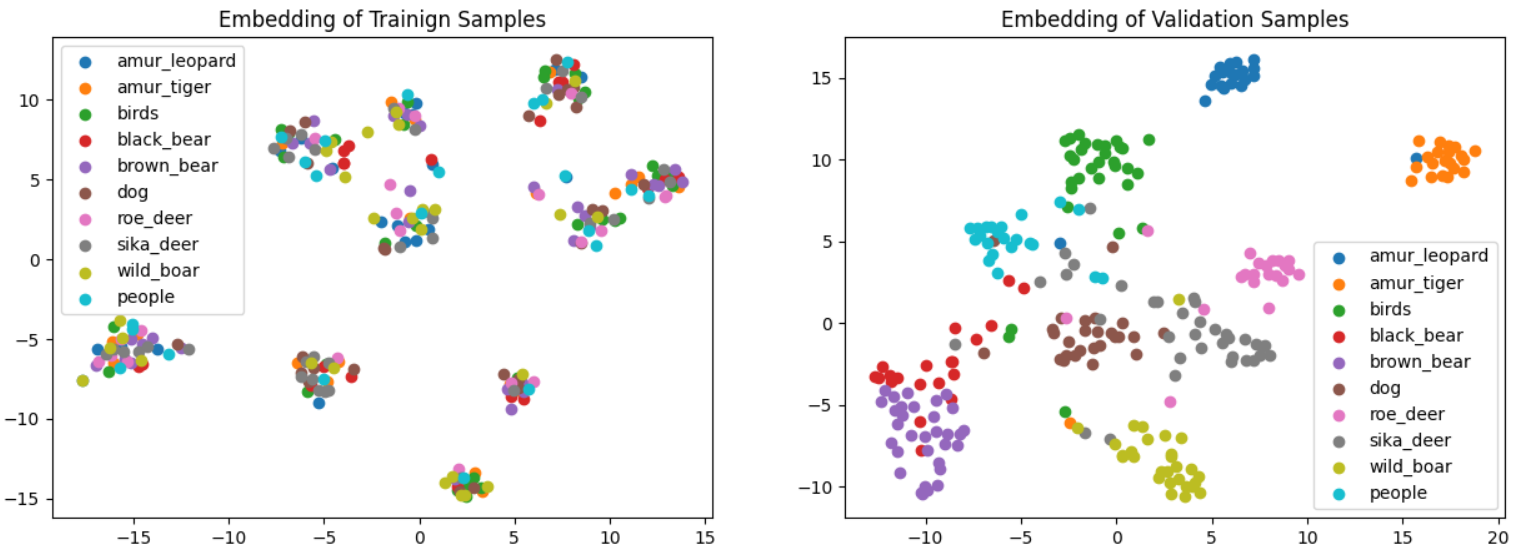
\includegraphics[width=0.9\textwidth]{Assets/Classification/Resnet/06}
            \caption{2D $t$-SNE visualizations of the training and validation set}
            \label{fig:resnet-tsne-2d}
        \end{figure}
        \begin{figure}[h!]
            \centering
            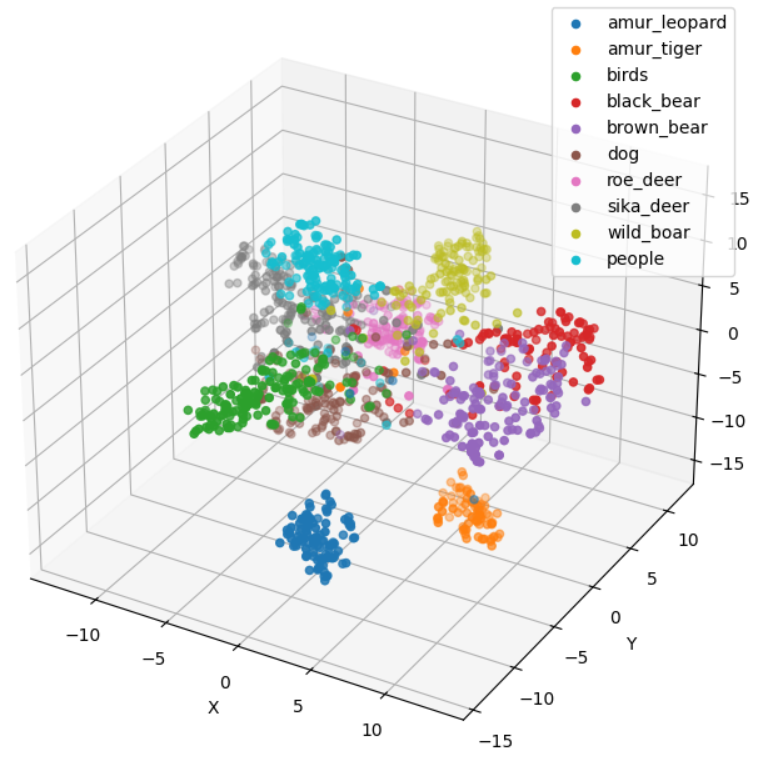
\includegraphics[width=0.5\textwidth]{Assets/Classification/Resnet/07}
            \caption{3D $t$-SNE visualizations of the validation set}
            \label{fig:resnet-tsne-3d}
        \end{figure}
    \end{enumerate}

    \subsection*{\textbf{Question 4.}}
    \begin{enumerate}[label=(\alph*)]
        \item To perform data augmentation to increase robustness of the model, I used different
        transforms to add randomness in the data, which are available in \texttt{torchvision.transforms}.
        Specifically, I applied random affine transforms, random horizontal flipping with probability
        0.5 for each image, and added random color noise or jitter in the images, altering their
        color schemes (brightness, contrast, saturation, and hue). A total of 2000 augmented images were
        added to the dataset.
        \item As asked in the Question, the same steps as \textbf{Question 2.3 (a)} were
        followed to train the Resnet-18 model on the augmented dataset.
        \item Looking at the loss curves, it is clear that this model performs even better
        than before, and is not overfitting. The per epoch loss/accuracy curves generated using wandb
        are given in Figure (\ref{fig:resnet-aug-loss-accuracy-curves}).
        \begin{figure}[h!]
            \centering
            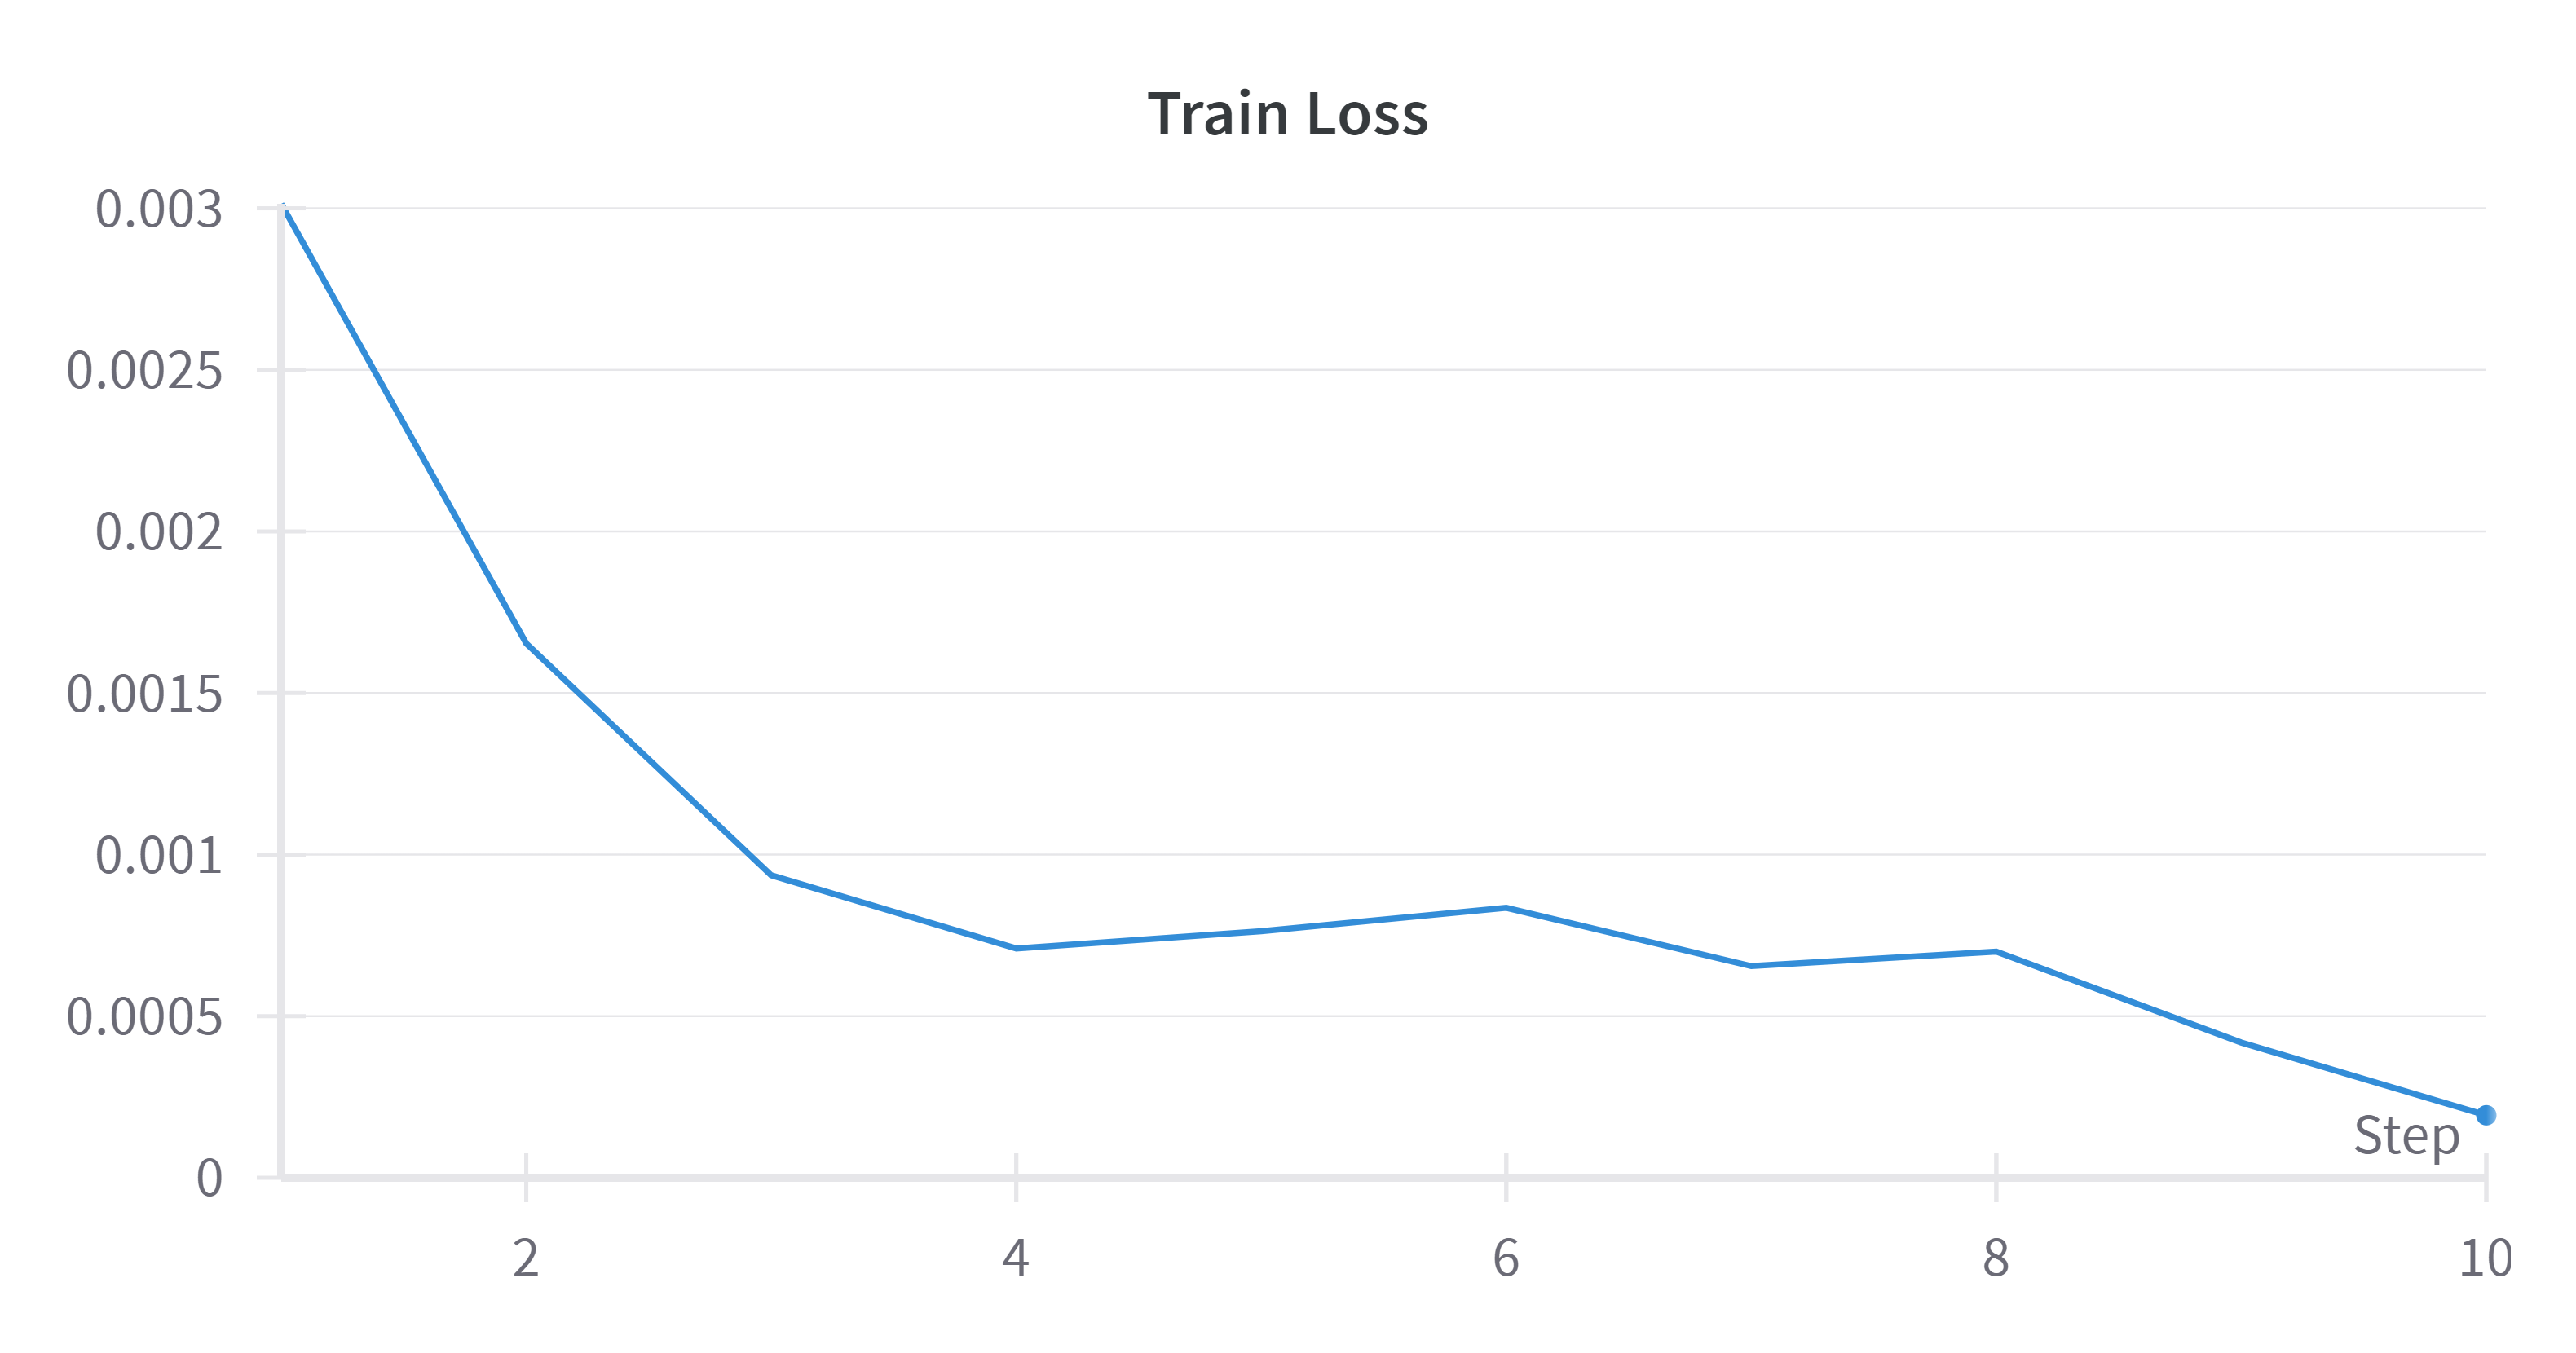
\includegraphics[width=0.4\textwidth]{Assets/Classification/Resnet-Aug/01}
            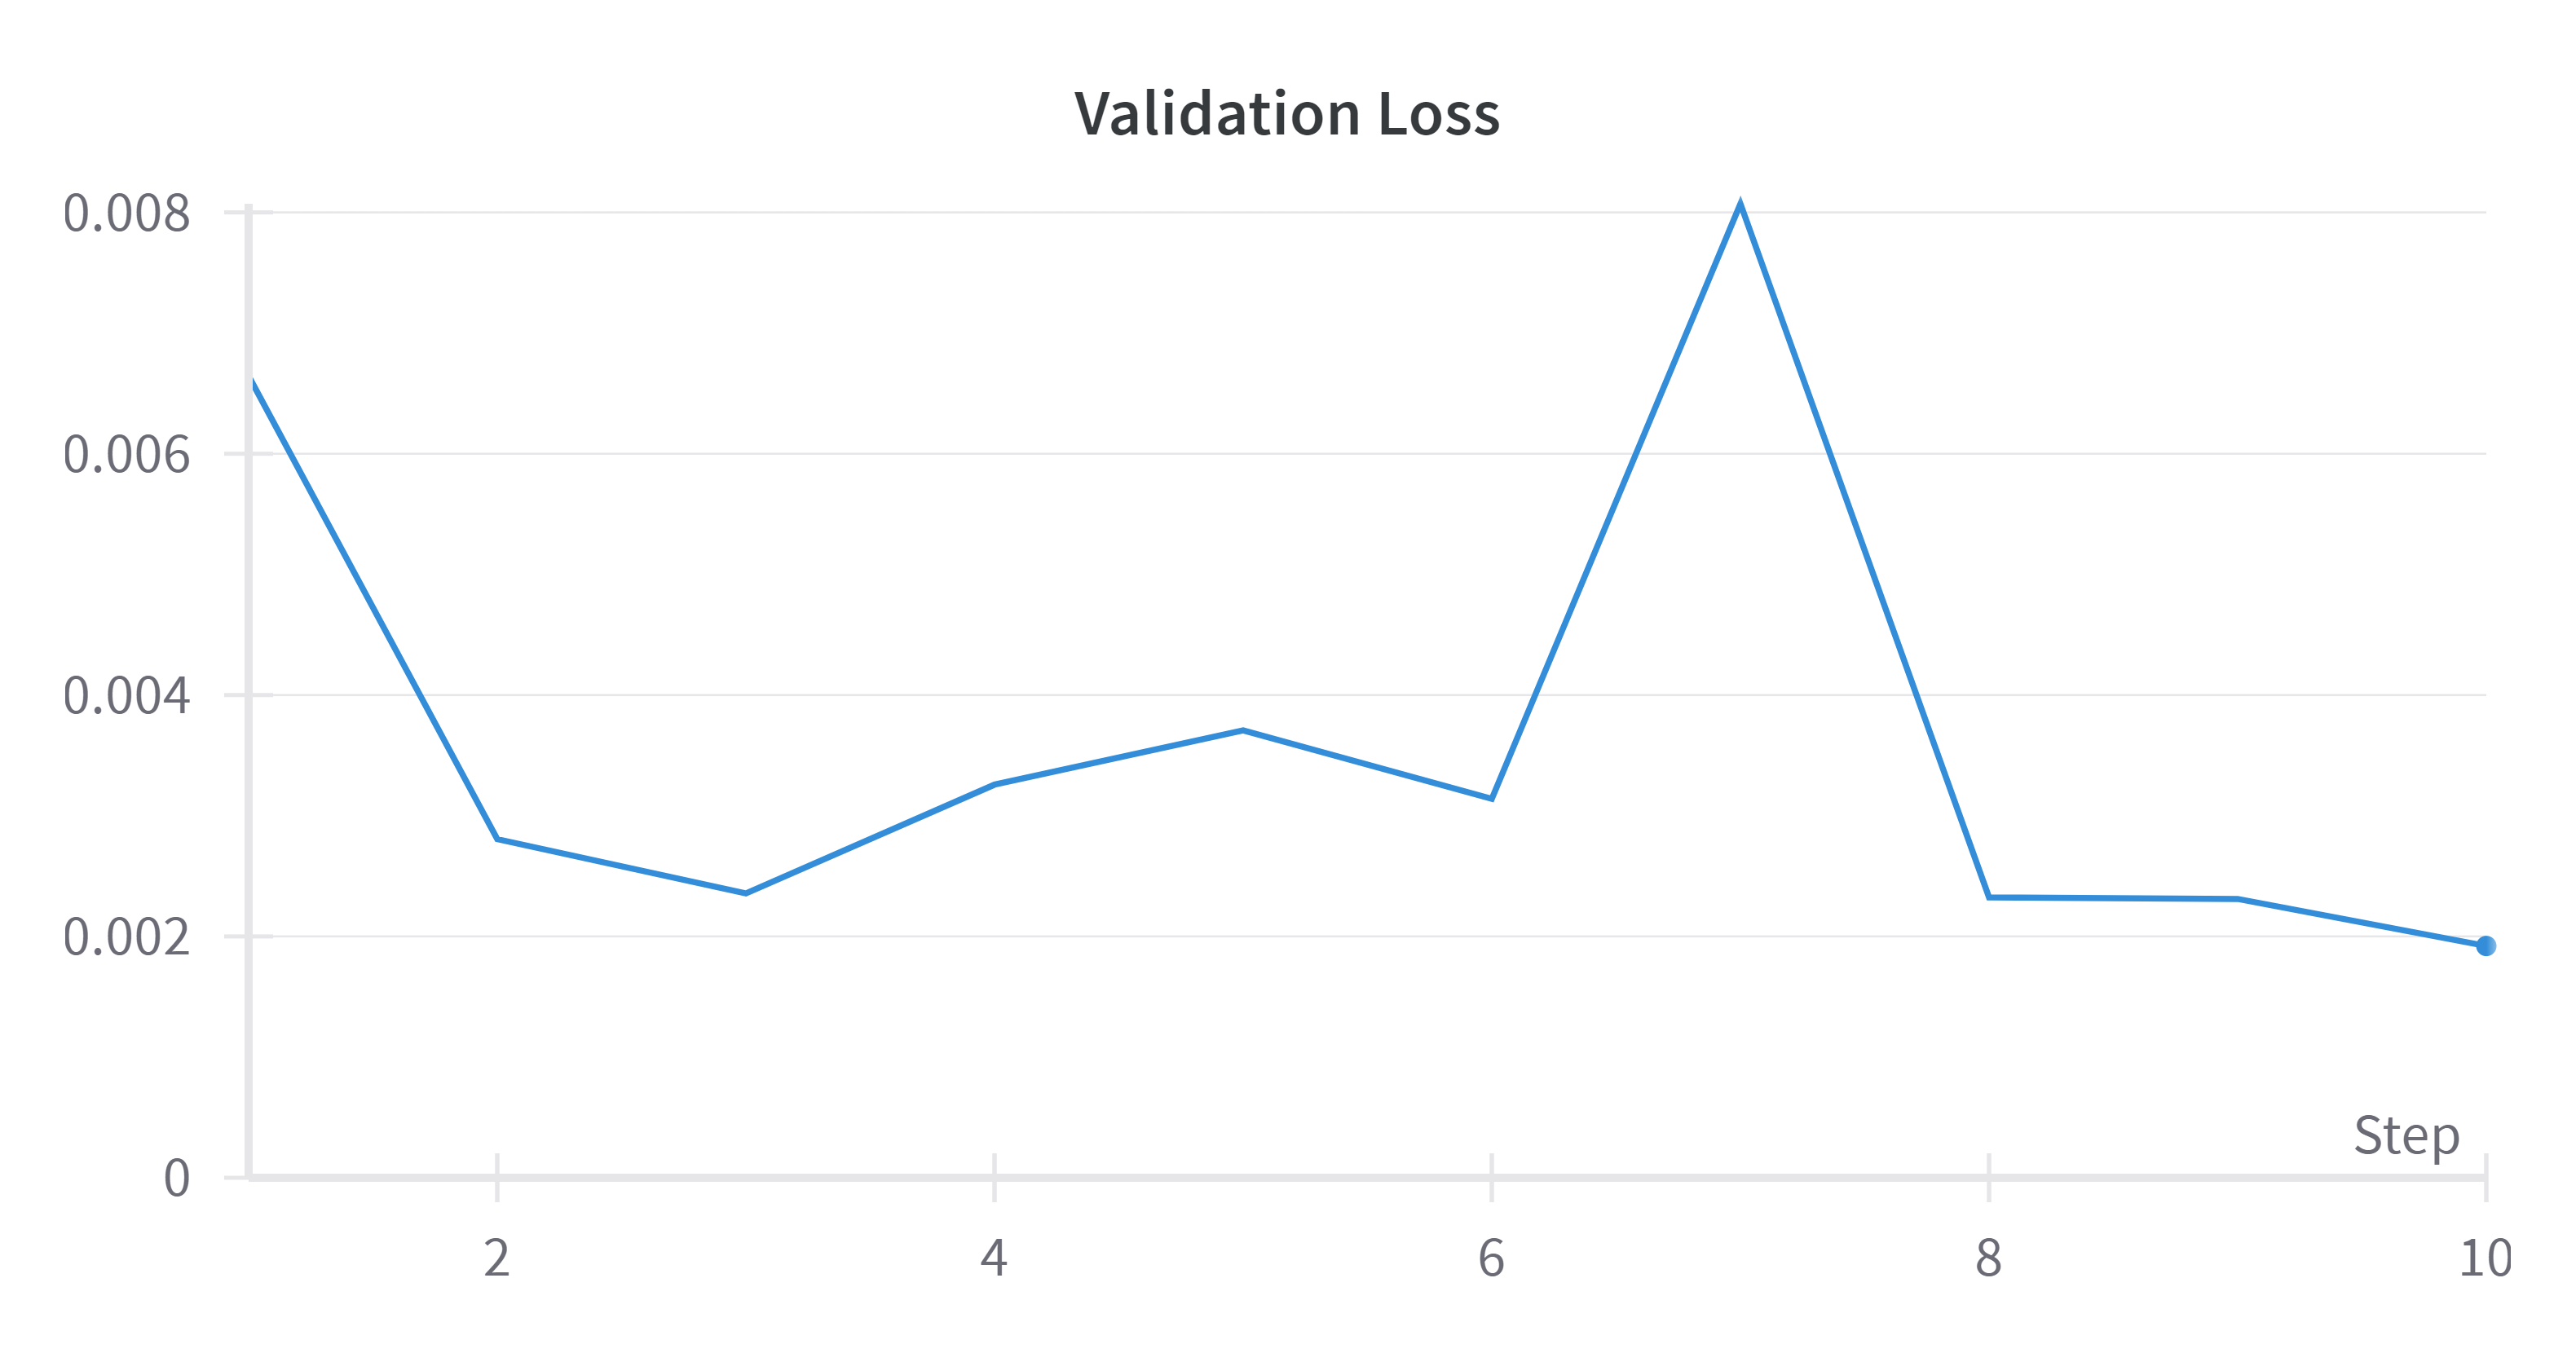
\includegraphics[width=0.4\textwidth]{Assets/Classification/Resnet-Aug/02}
            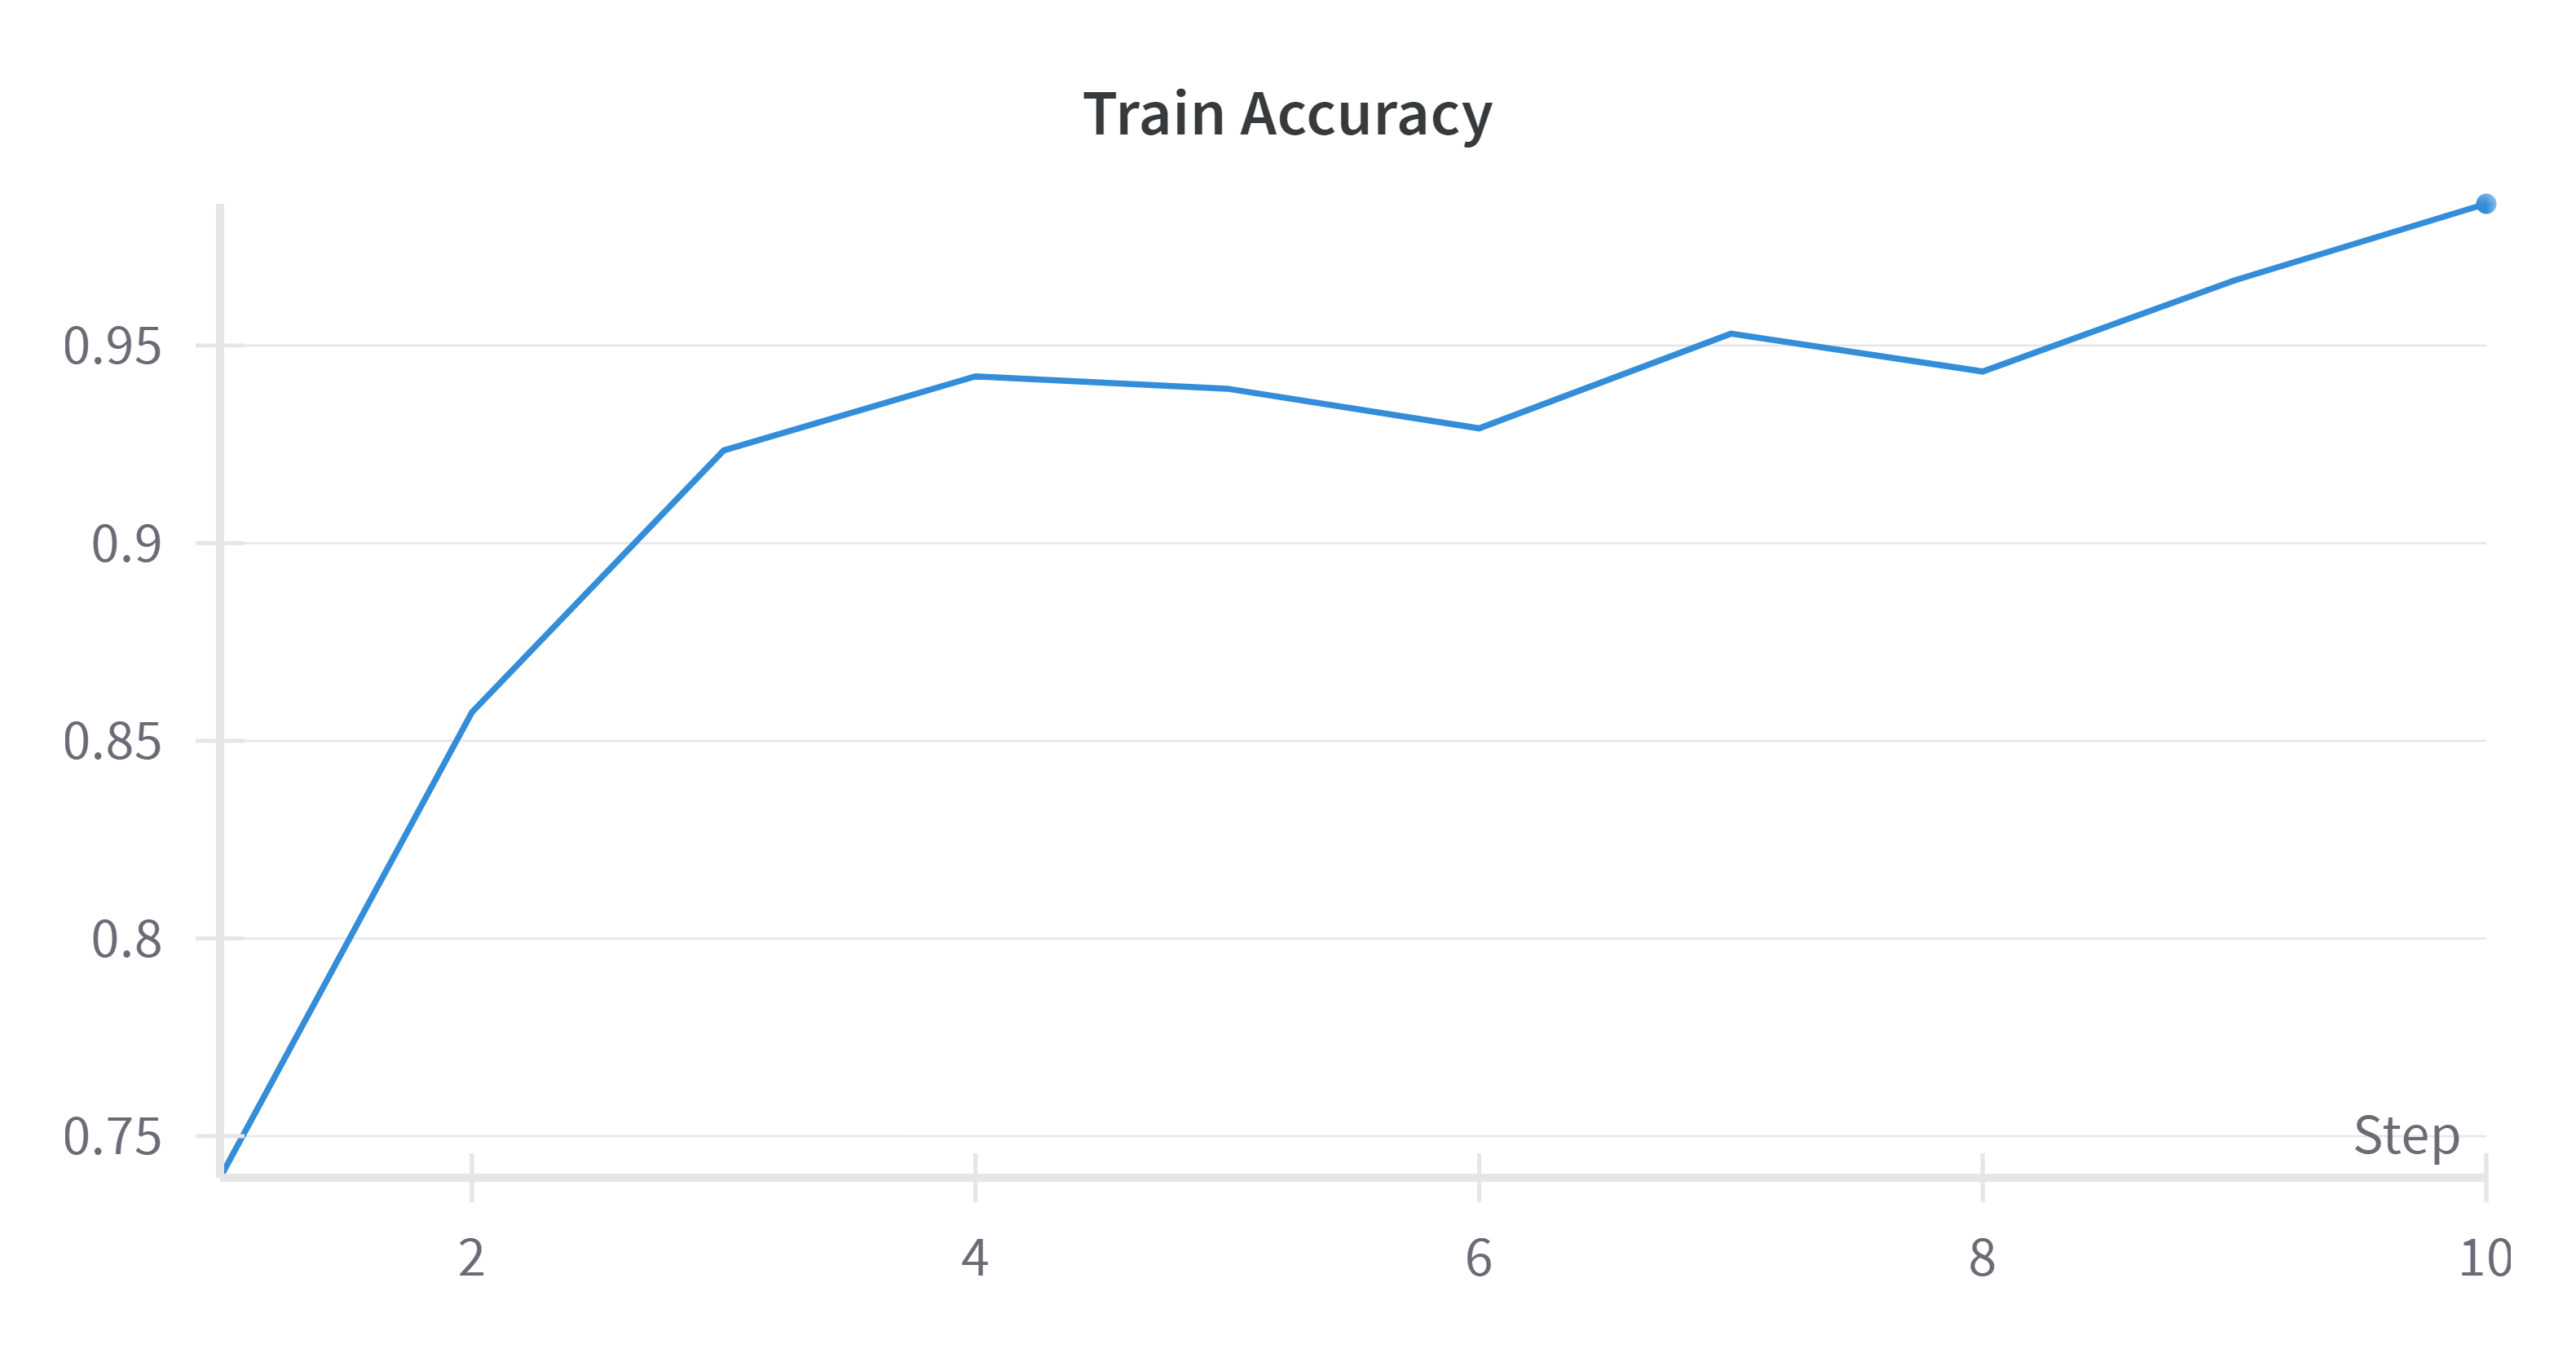
\includegraphics[width=0.4\textwidth]{Assets/Classification/Resnet-Aug/03}
            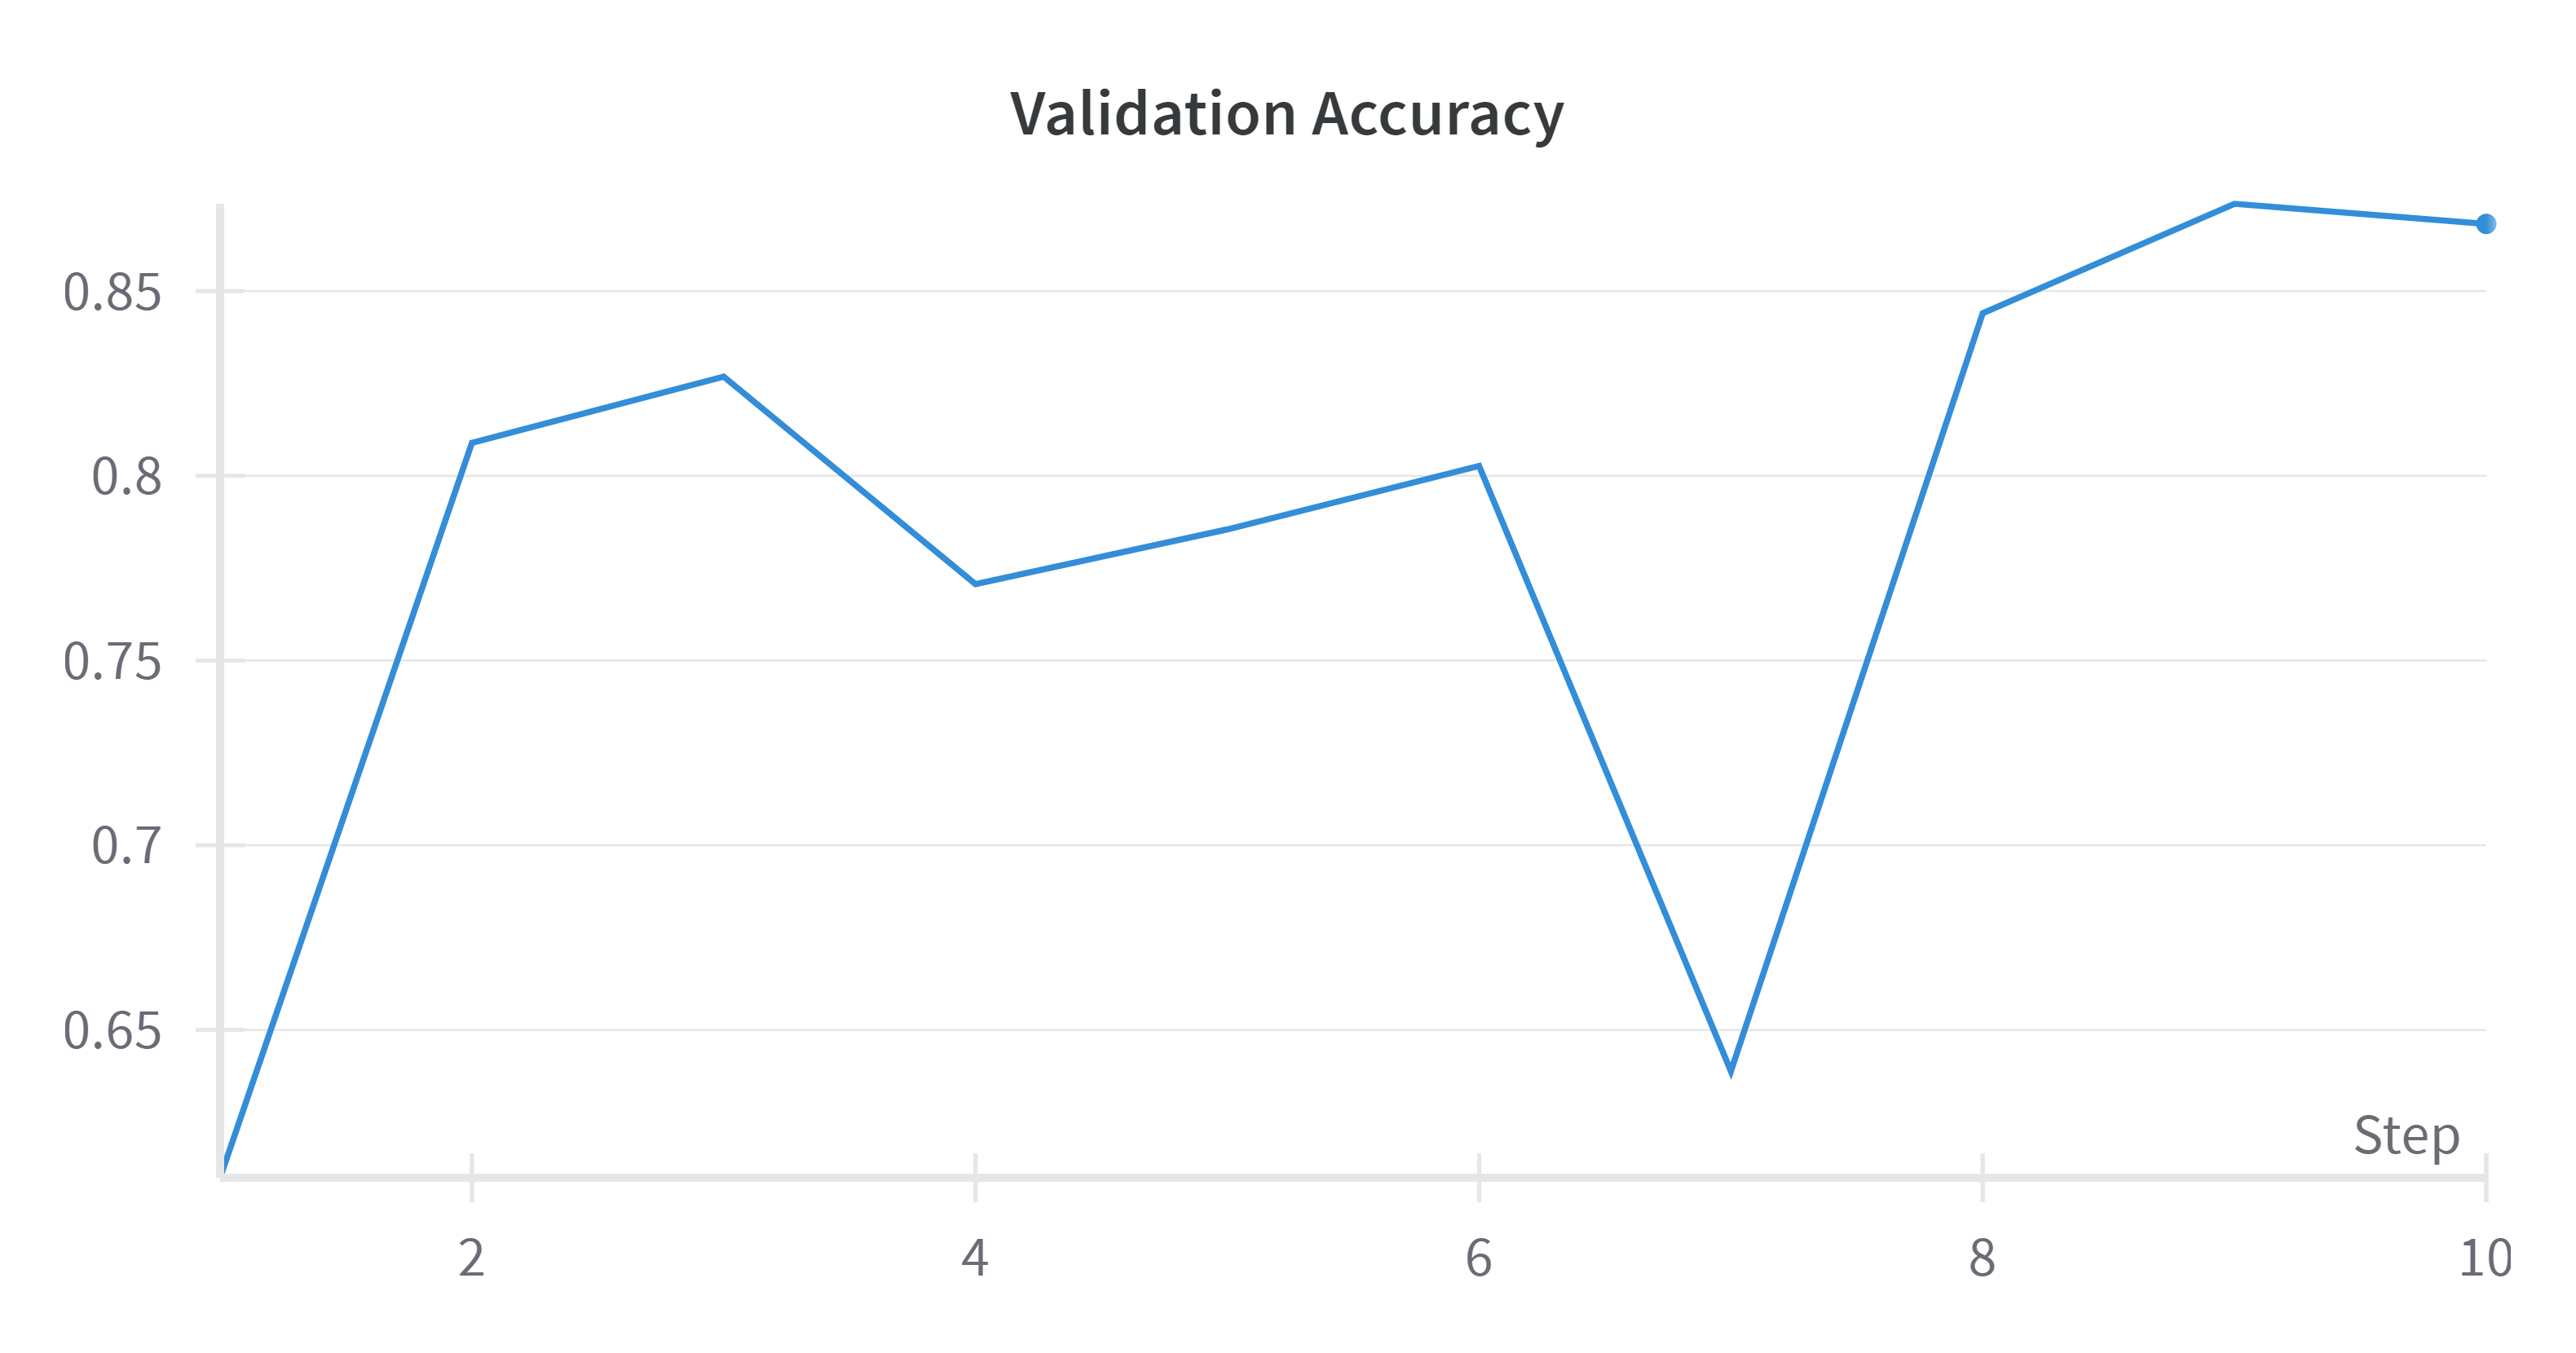
\includegraphics[width=0.4\textwidth]{Assets/Classification/Resnet-Aug/04}
            \caption{Loss and Accuracy curves (per epoch) for Resnet-18 architecture (on augmented dataset)}
            \label{fig:resnet-aug-loss-accuracy-curves}
        \end{figure}
        \item The Resnet-18 mmodel finetuned on the augmented dataset performed marginally better than
        the previous model. It achieved an accuracy of 0.976+. The precision, recall, and F1-score for
        the classification all turned out to be 0.883+. The confusion matrix (logged using wandb) is given
        in Figure (\ref{fig:resnet-aug-conf-matrix}).
        \begin{figure}[h!]
            \centering
            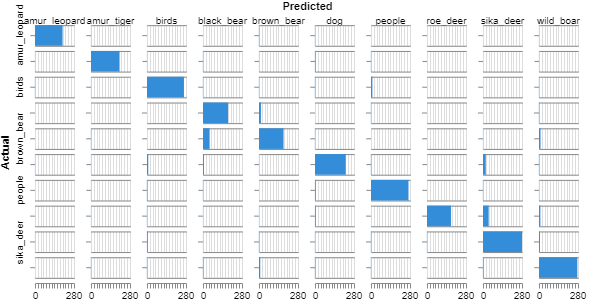
\includegraphics[width=0.7\textwidth]{Assets/Classification/Resnet-Aug/05}
            \caption{Confusion Matrix for the Resnet-18 architecture (on augmented dataset)}
            \label{fig:resnet-aug-conf-matrix}
        \end{figure}
    \end{enumerate}

    \subsection*{\textbf{Question 5.}}
    The analysis for this question is also given in the notebook. The euclidean distances
    between the feature space representations of the misclassified images were calculated
    from the mean of both the ground truth and predicted classes. It is interesting to note
    that in some cases, the distance to the mean of the ground truth class was lower than
    the distance to the mean of the predicted class. However, such cases were rare.
    A few examples are given in Figure (\ref{fig:dists}).
    \begin{figure}[h!]
        \centering
        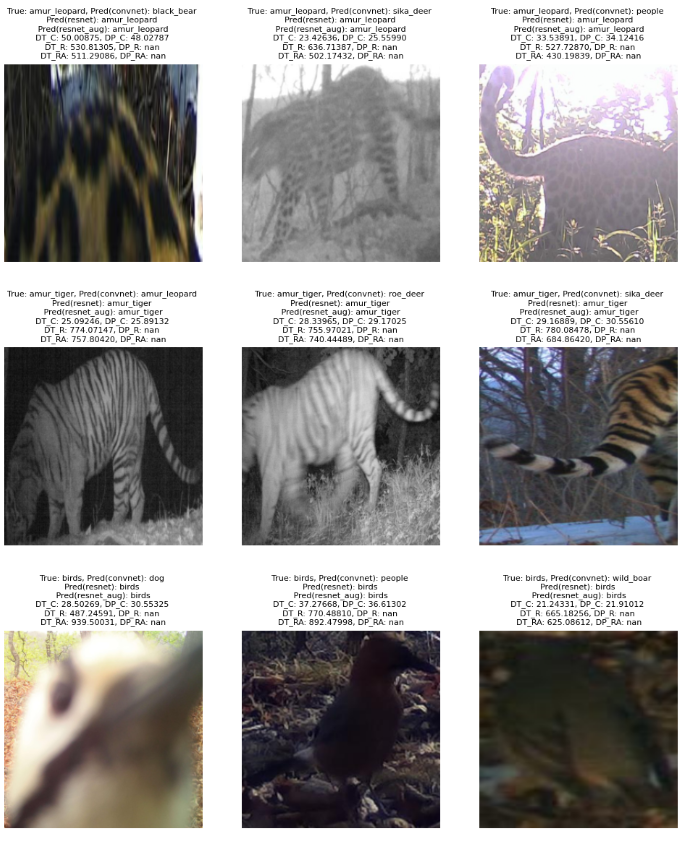
\includegraphics[width=0.325\textwidth]{Assets/Classification/Convnet/Misclassifications/04}
        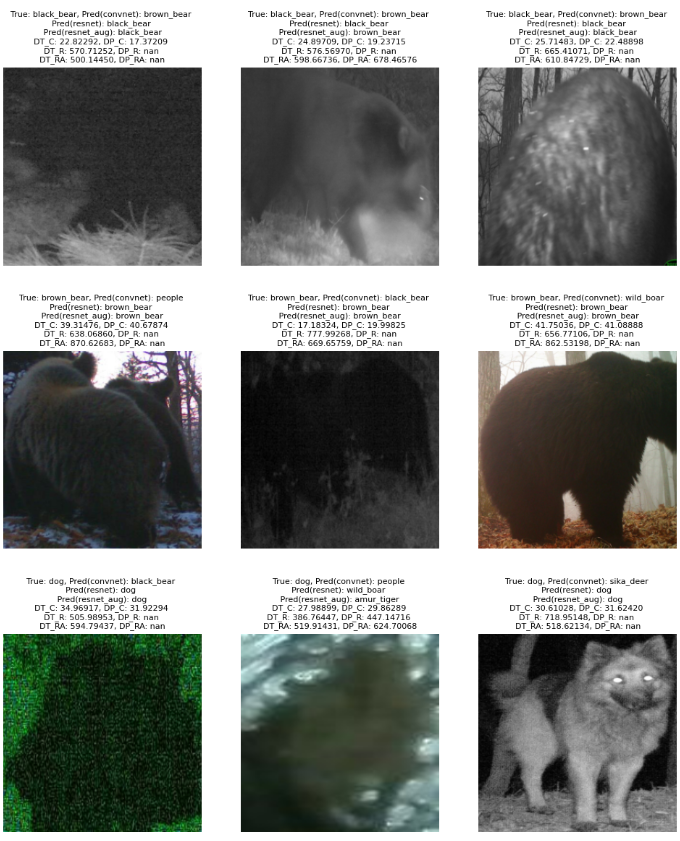
\includegraphics[width=0.325\textwidth]{Assets/Classification/Convnet/Misclassifications/05}
        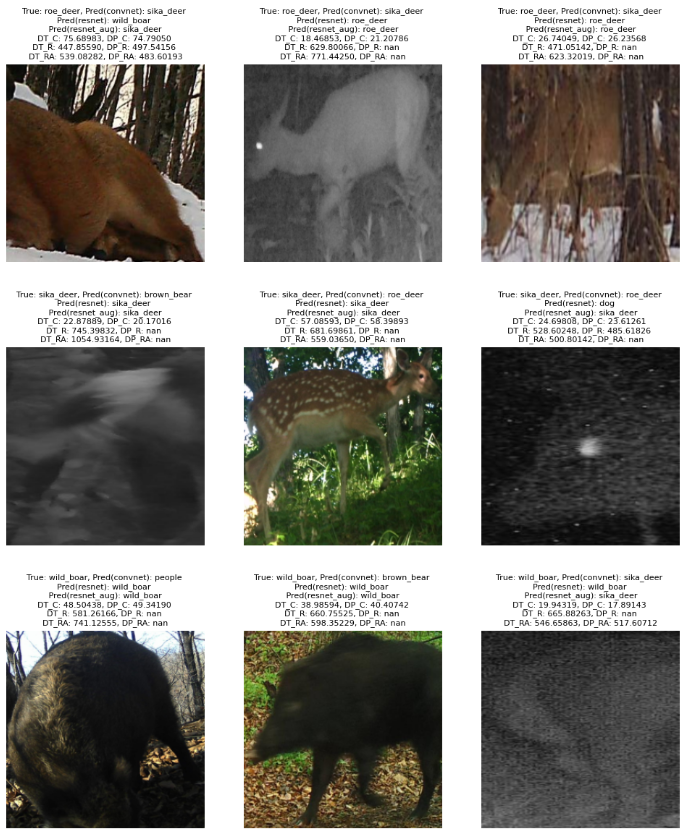
\includegraphics[width=0.325\textwidth]{Assets/Classification/Convnet/Misclassifications/06}
        \caption{Euclidean distances of misclassified images to centroids of predicted and true classes}
        \label{fig:dists}
    \end{figure}

    \subsection*{\textbf{Question 6.}}
    On comparing all the three models, it is pretty clear that the vanilla CNN architecture
    performs well, but not as well as we would like. Its recall and F1-scores are low. This
    is due to its comparitively lower capacity and higher tendency to overfit the data. On the
    flip side, the Resnet-18 architectures performed extremely well. Both models did not
    overfit, achieving high scores for all common evaluation metrics. The model trained with
    the augmented dataset outperformed the other one by a small margin, since adding some noise
    to the dataset increases its ability to generalize.

    \section*{\textbf{Image Segmentation}}
    The solutions to the questions in this section are given in two notebooks,
    namely \texttt{segmentation-1.ipynb} and \texttt{segmentation-2.ipynb} (By this
    time, I figured out connecting Google Drive to Google Colab, and hence the second
    notebook performed inferences using the GPU).

    \subsection*{\textbf{Question 1.}}
    \begin{enumerate}[label=(\alph*)]
        \item Similar to the image classification problem, I created a custom dataset
        class, \texttt{IDD}, which also handles label mappings and mask color mappings for
        both the IDD and Cityscapes dataset. Since the images were larger in size, I used
        a batch size of 8 to create the dataloader. The dataset was imported from Google Drive :)
        \item To visualize the data distribution across the dataset, I used pixel counts in
        the masks - the frequency of pixels belonging to each of the classes. Due to computational
        limitations, the plot was generated only for a fraction of the dataset. The distribution
        is given in Figure (\ref{fig:pixel-counts}).
        \begin{figure}[h!]
            \centering
            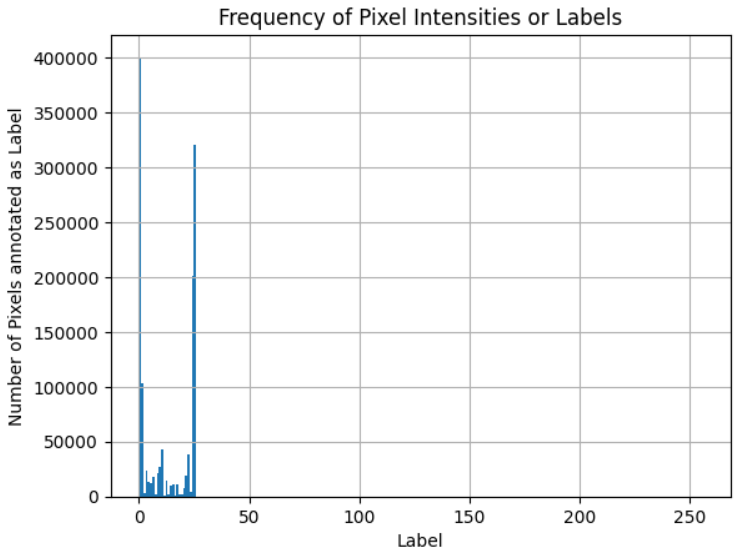
\includegraphics[width=0.4\textwidth]{Assets/Segmentation/01}
            \caption{Pixel Counts of each class (representing data distribution)}
            \label{fig:pixel-counts}
        \end{figure}
        \item For each class, I visualize the images and their masks (and show which class
        is being highlighted in each case). The masks were color coded according to the conventions
        of the IDD Dataset. The results are given in \texttt{segmentation-1.ipynb}, and a few
        examples are given in Figure (\ref{fig:masks}).
        \begin{figure}[h!]
            \centering
            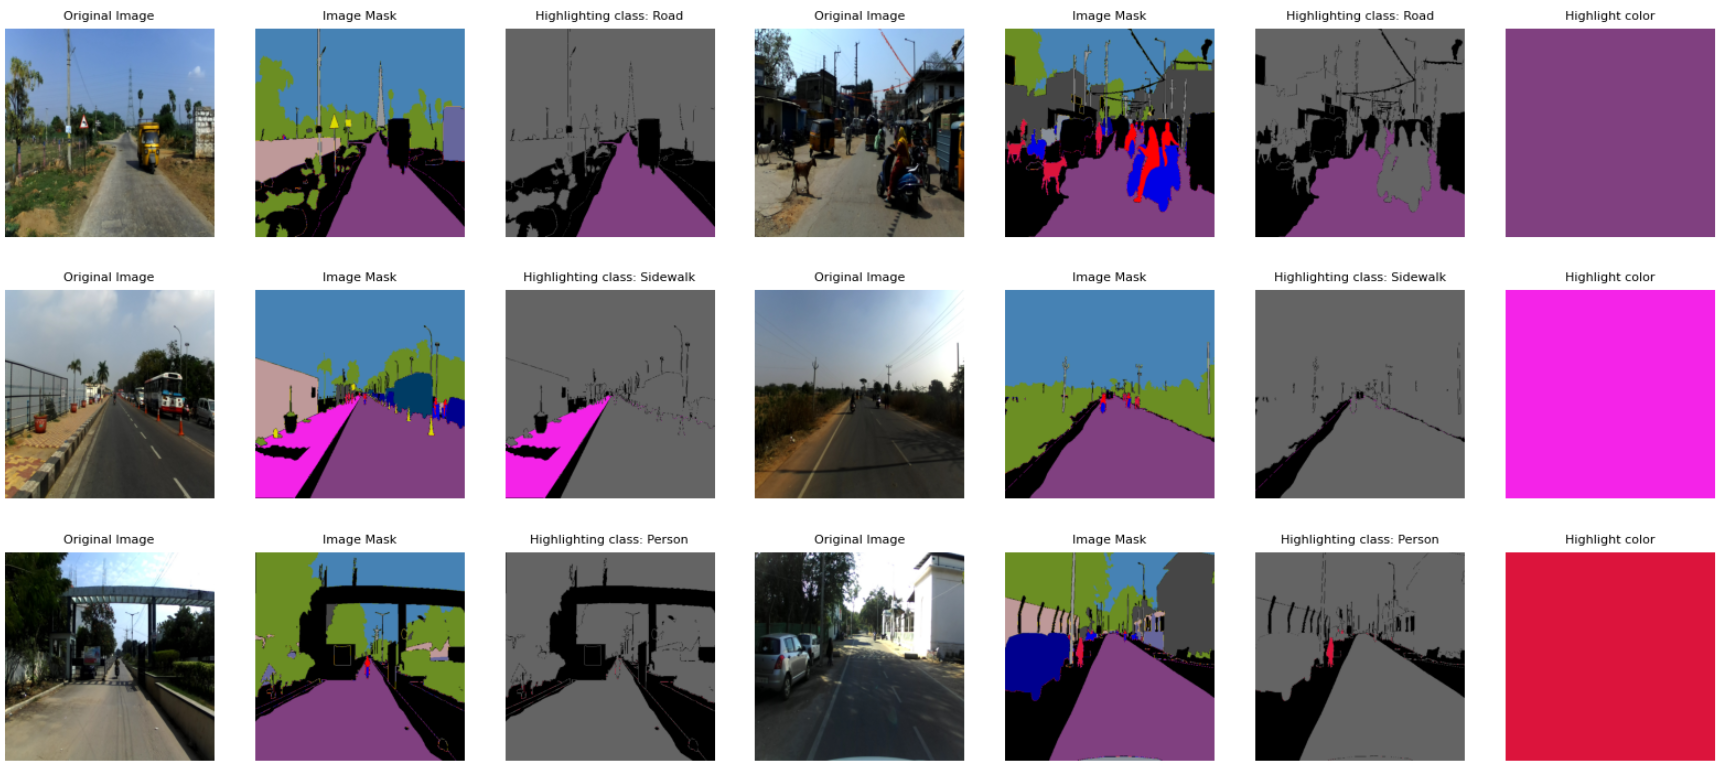
\includegraphics[width=0.325\textwidth]{Assets/Segmentation/Original/02}
            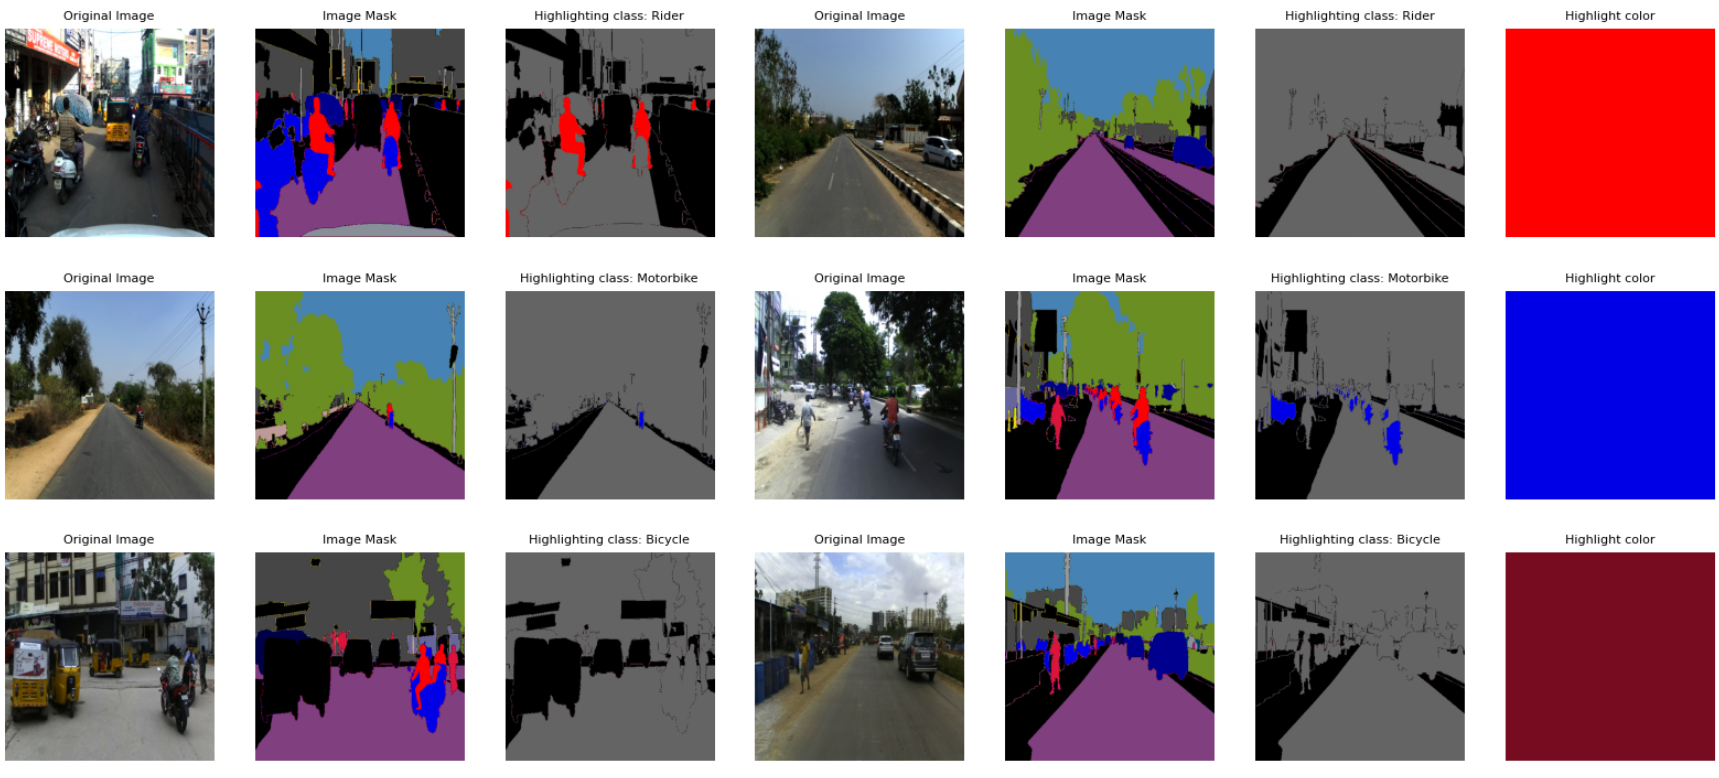
\includegraphics[width=0.325\textwidth]{Assets/Segmentation/Original/03}
            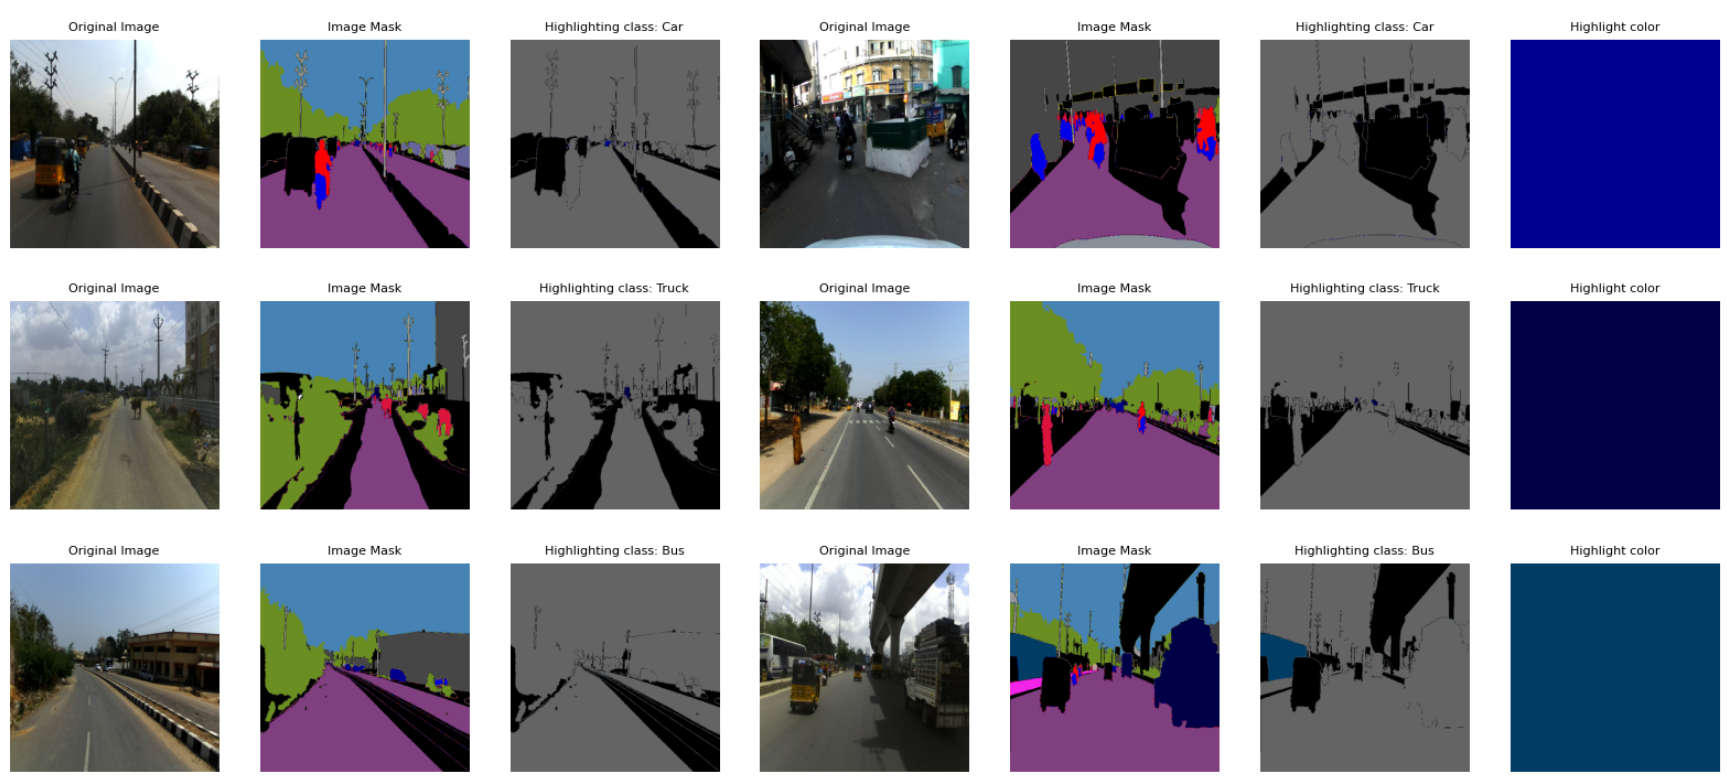
\includegraphics[width=0.325\textwidth]{Assets/Segmentation/Original/04}
            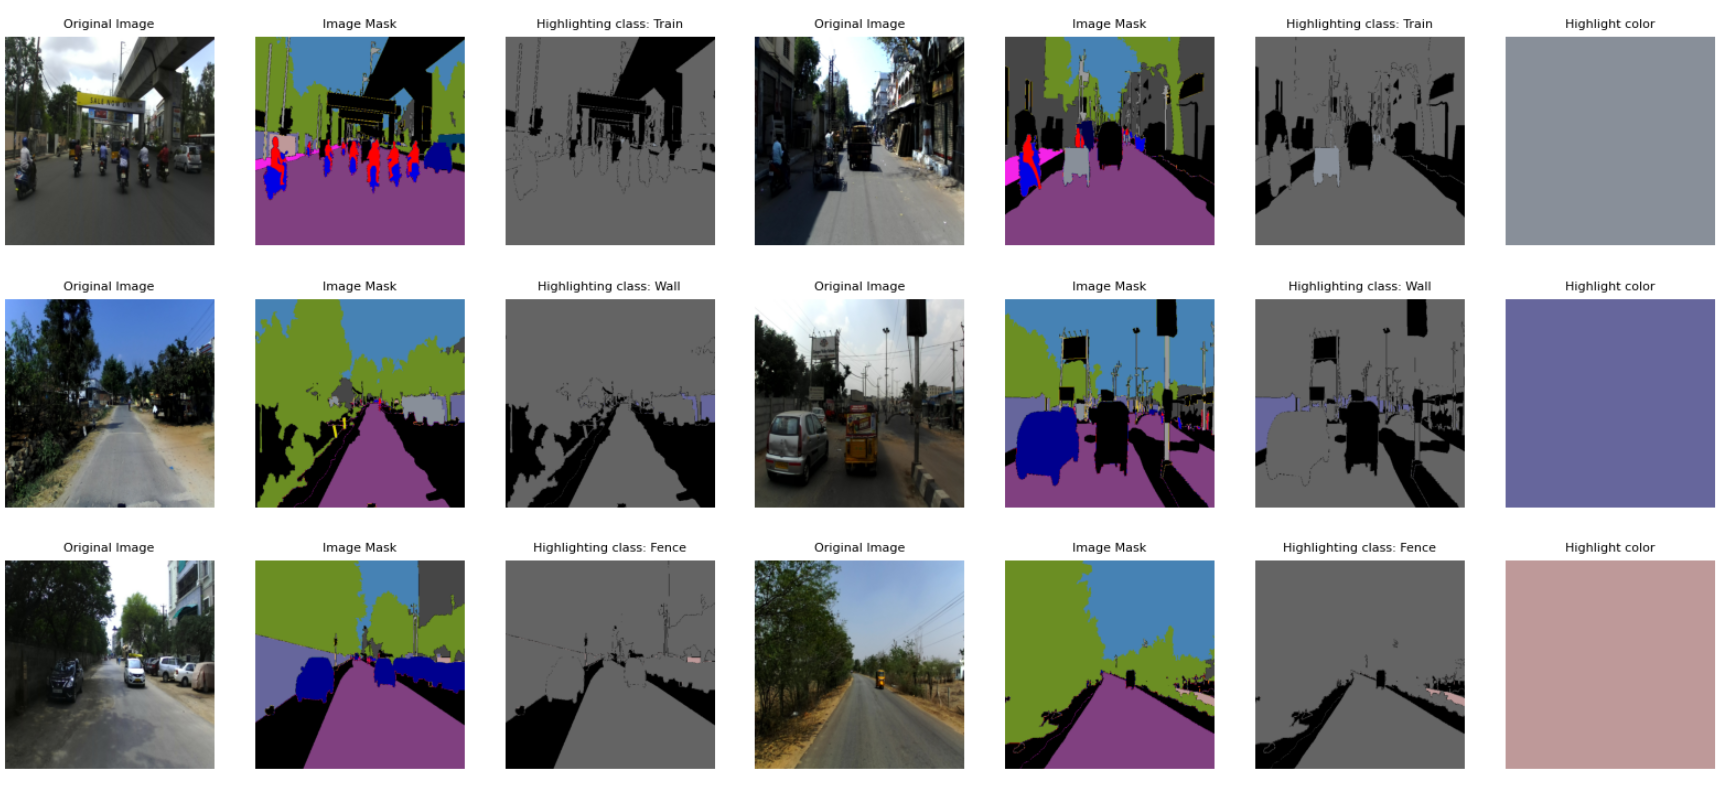
\includegraphics[width=0.325\textwidth]{Assets/Segmentation/Original/05}
            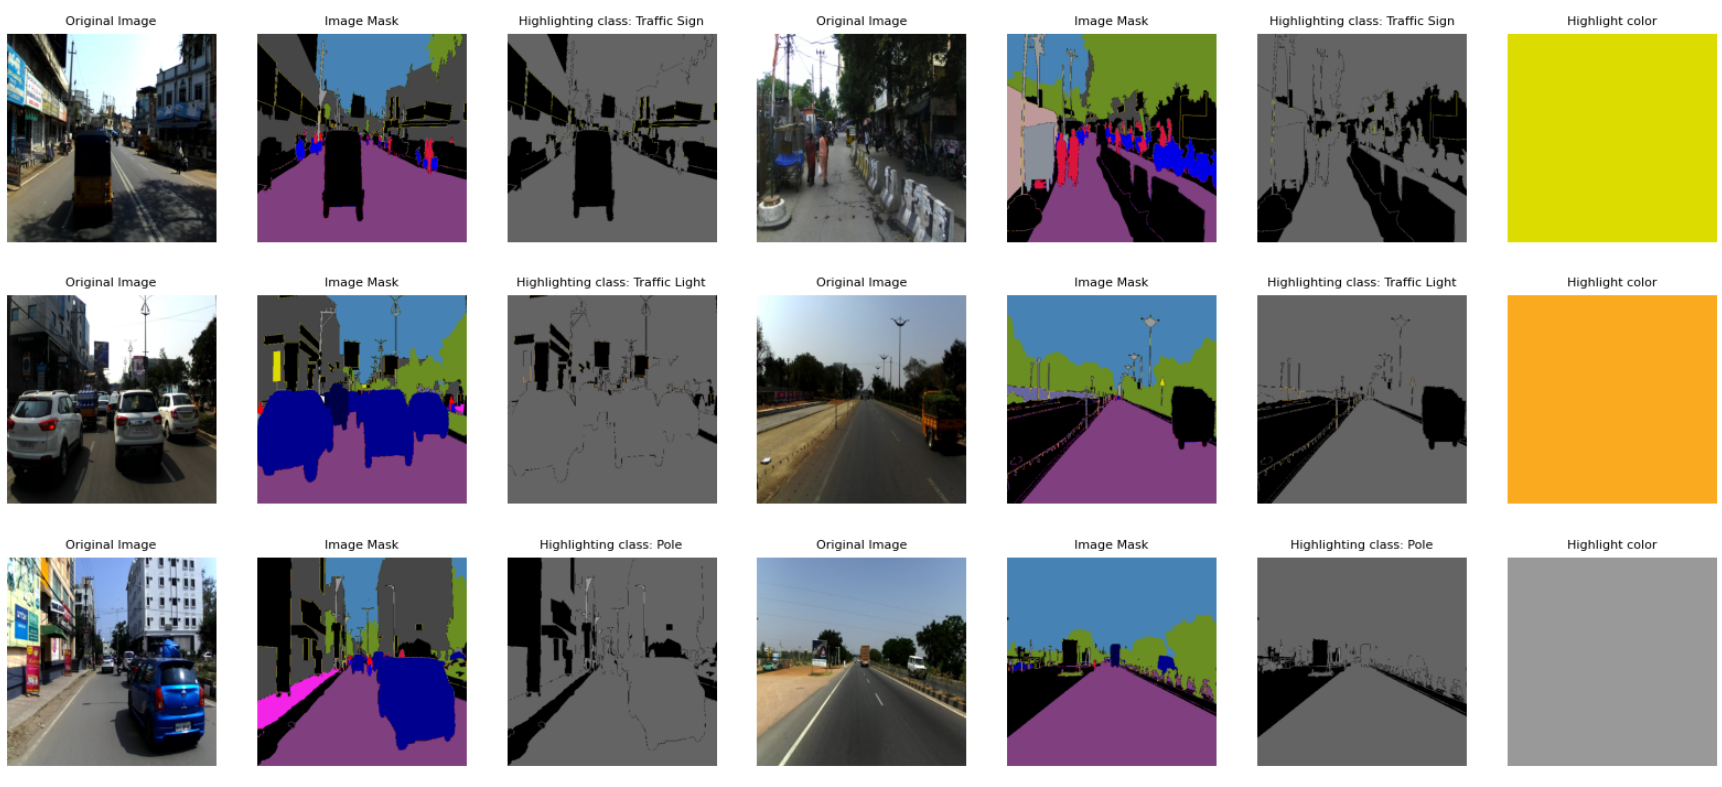
\includegraphics[width=0.325\textwidth]{Assets/Segmentation/Original/06}
            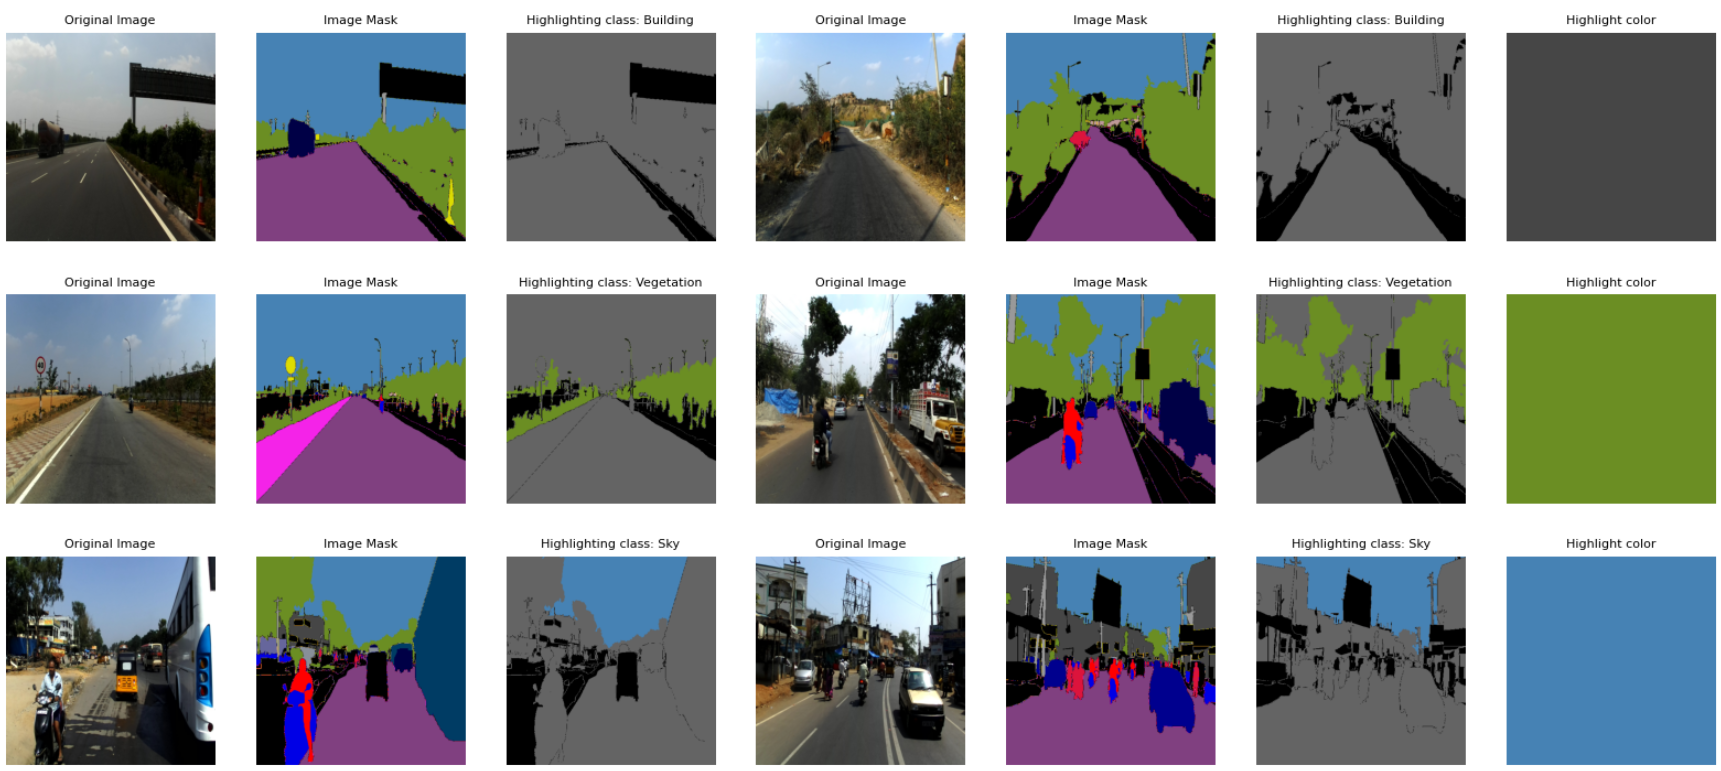
\includegraphics[width=0.325\textwidth]{Assets/Segmentation/Original/07}
            \caption{Visualization of three images of every class}
            \label{fig:masks}
        \end{figure}
    \end{enumerate}

    \subsection*{\textbf{Question 2.}}
    \begin{enumerate}[label=(\alph*)]
        \item The DeepLabv3Plus-PyTorch Resnet-101 model was used for performing inferences
        on 30\% IDD dataset (using it as test set). The inference was performed in the second
        notebook, which is GPU enabled.
        \item The classwise performances in terms of the given metrics were evaluated. The results
        are given in Figure (\ref{fig:metrics-screenshot}) (Forgive me, I did not have enough time to
        present these in a better manner).
        \begin{figure}[h!]
            \centering
            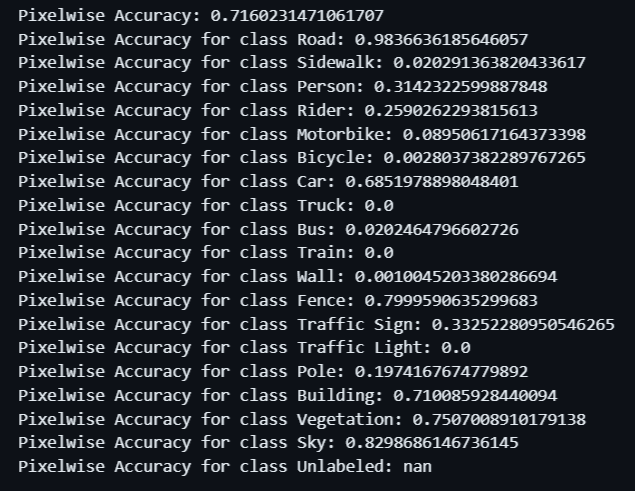
\includegraphics[width=0.325\textwidth]{Assets/Segmentation/Metrics/01}
            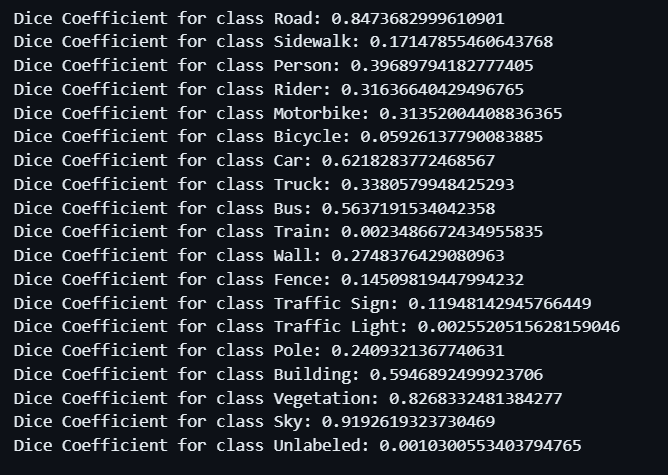
\includegraphics[width=0.335\textwidth]{Assets/Segmentation/Metrics/02}
            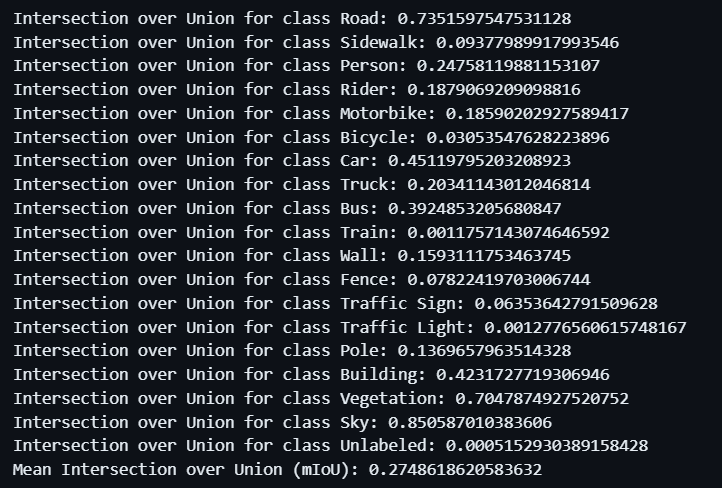
\includegraphics[width=0.35\textwidth]{Assets/Segmentation/Metrics/03}
            \caption{Evaluation Metrics for the Image Segmentation}
            \label{fig:metrics-screenshot}
        \end{figure}
        \item I visualize three images per class where the IoU between the predicted and true
        masks is at most 0.5. It was easy to notice the faults - in some cases, the IoU was close to
        0.48+, for example, in case of \texttt{Road}. In other cases, like \texttt{Sidewalk} or
        \texttt{Traffic-Light}, the predicted masks did not contain these classes (hence the IoUs were 0).
        This is probably because the model was trained on a different and less complex dataset,
        resulting in classes that occur on only a few pixels per image to be \textit{ignored}.
        In such cases, the surrounding objects and environment were overpowering the ground truth
        class. For example, most pixels of \texttt{Sidewalk} were being predicted as \texttt{Road}.
        These \textit{bad IoU} examples are given in Figure (\ref{fig:bad-ious}).
        \begin{figure}[h!]
            \centering
            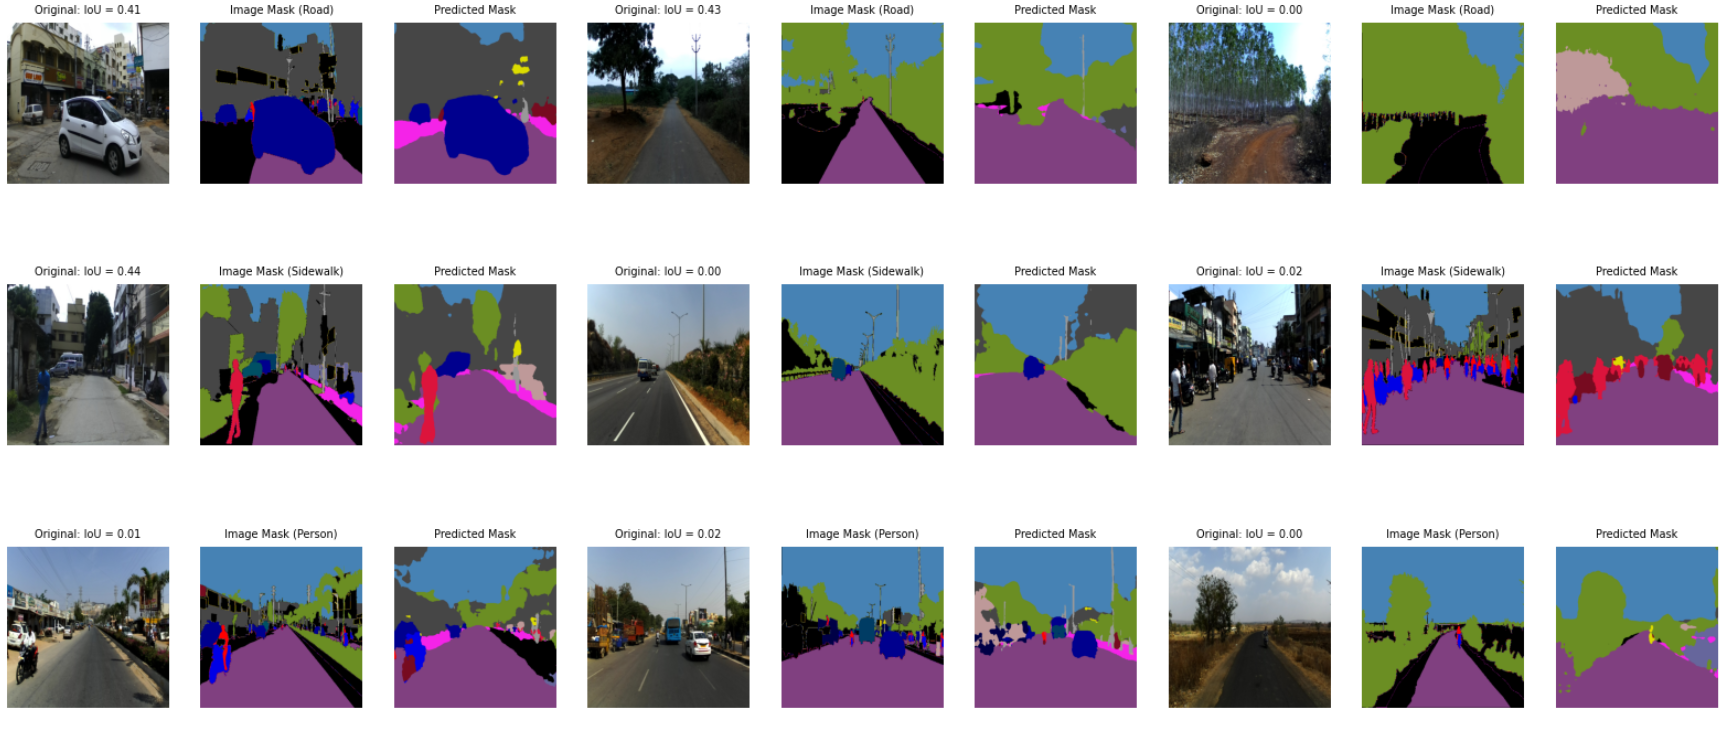
\includegraphics[width=0.325\textwidth]{Assets/Segmentation/Bad-IoUs/01}
            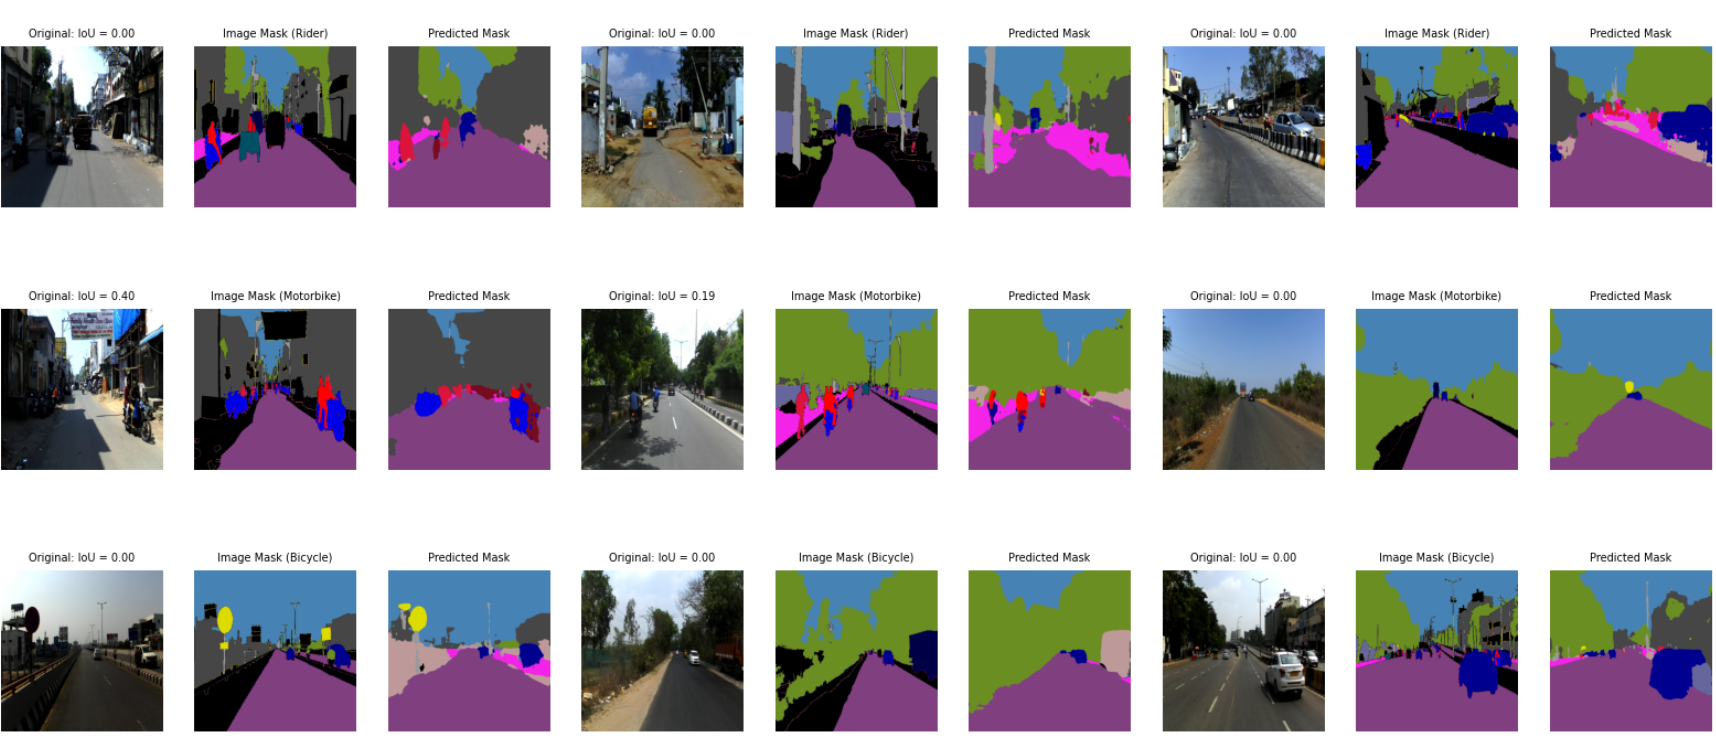
\includegraphics[width=0.325\textwidth]{Assets/Segmentation/Bad-IoUs/02}
            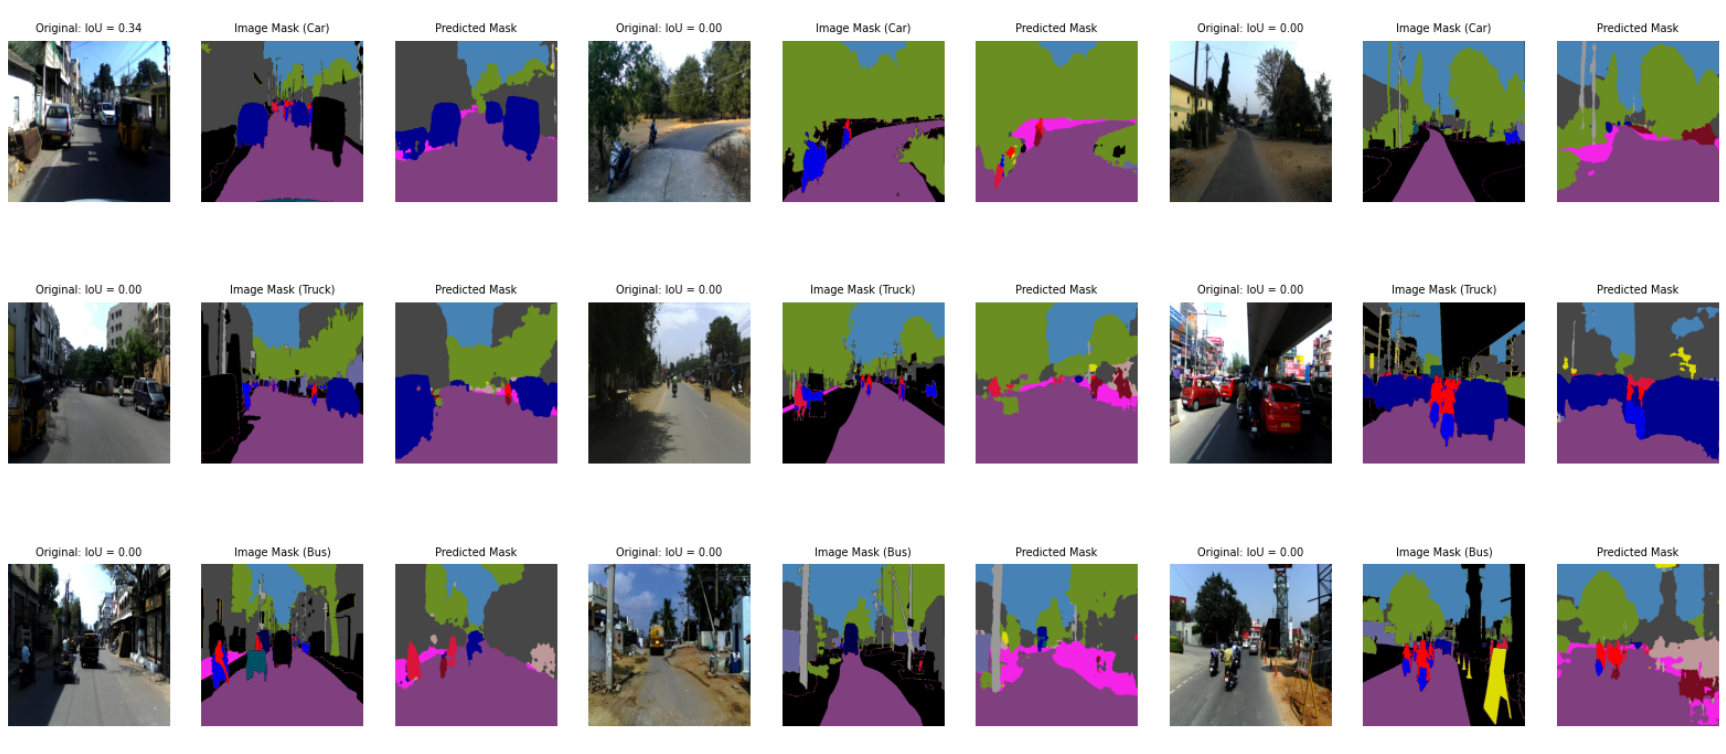
\includegraphics[width=0.325\textwidth]{Assets/Segmentation/Bad-IoUs/03}
            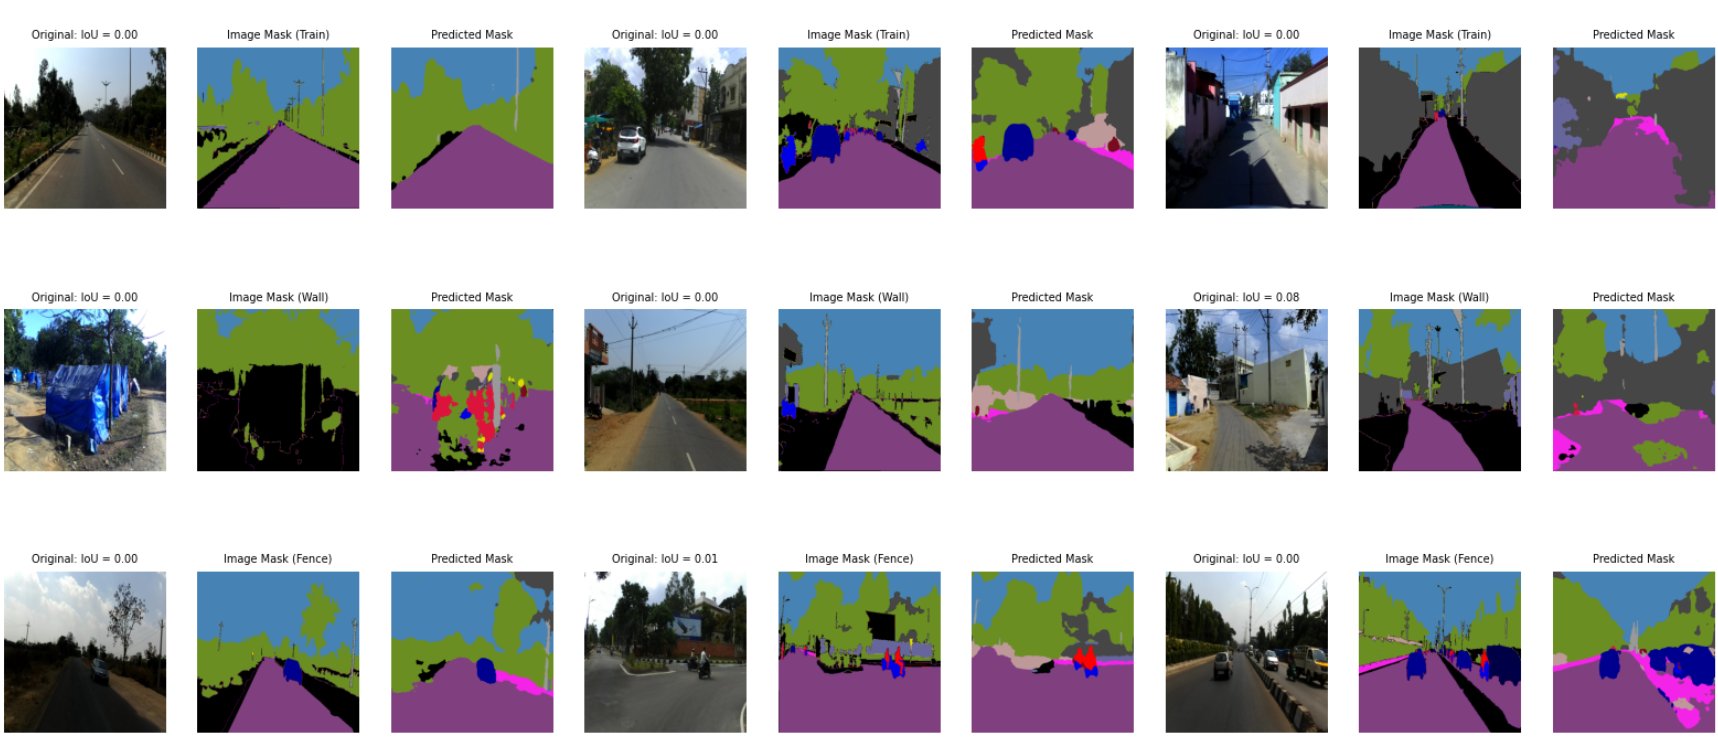
\includegraphics[width=0.325\textwidth]{Assets/Segmentation/Bad-IoUs/04}
            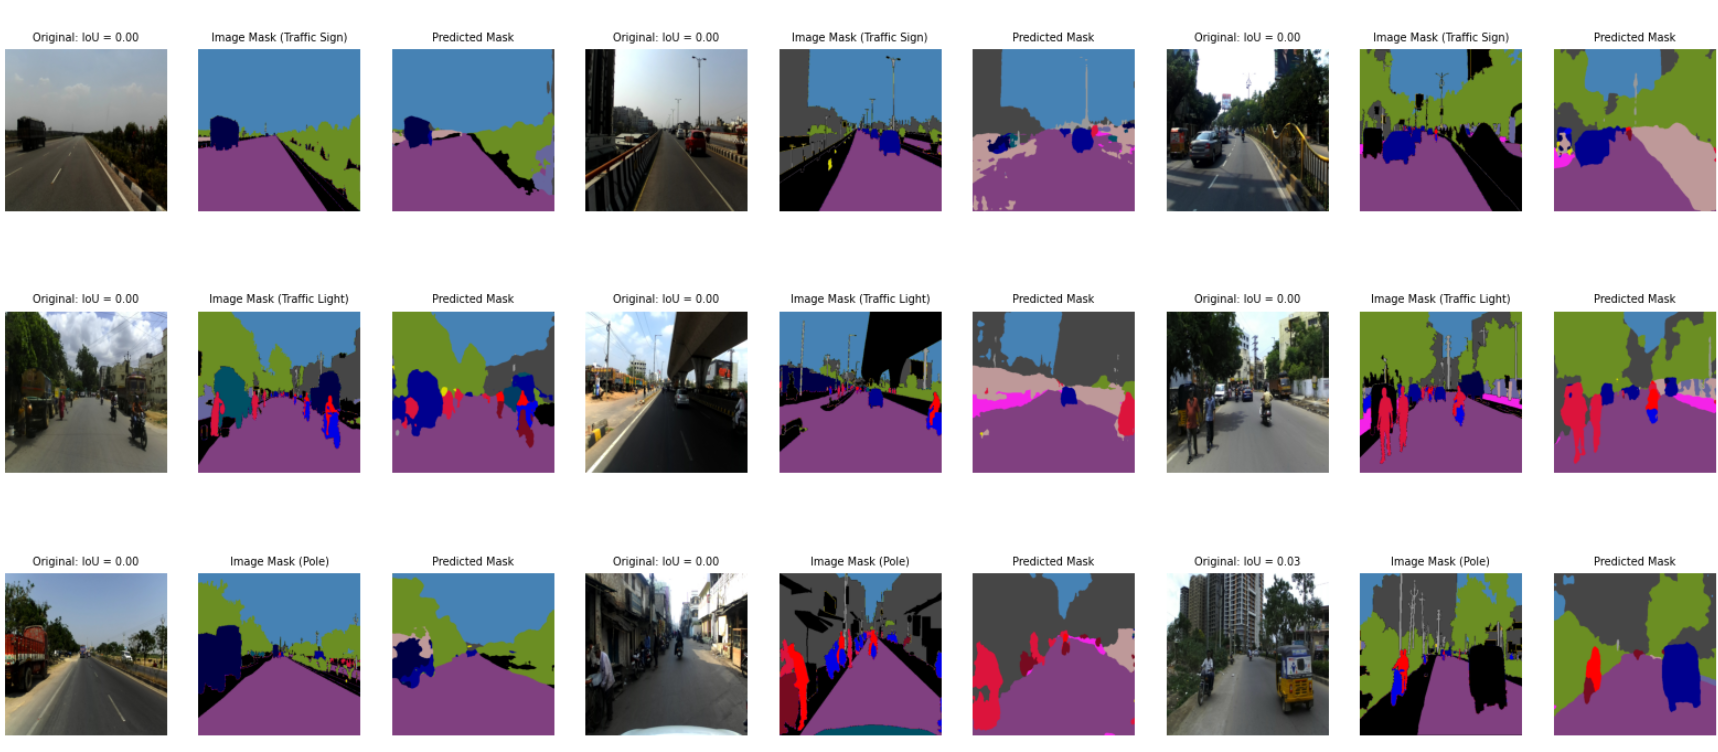
\includegraphics[width=0.325\textwidth]{Assets/Segmentation/Bad-IoUs/05}
            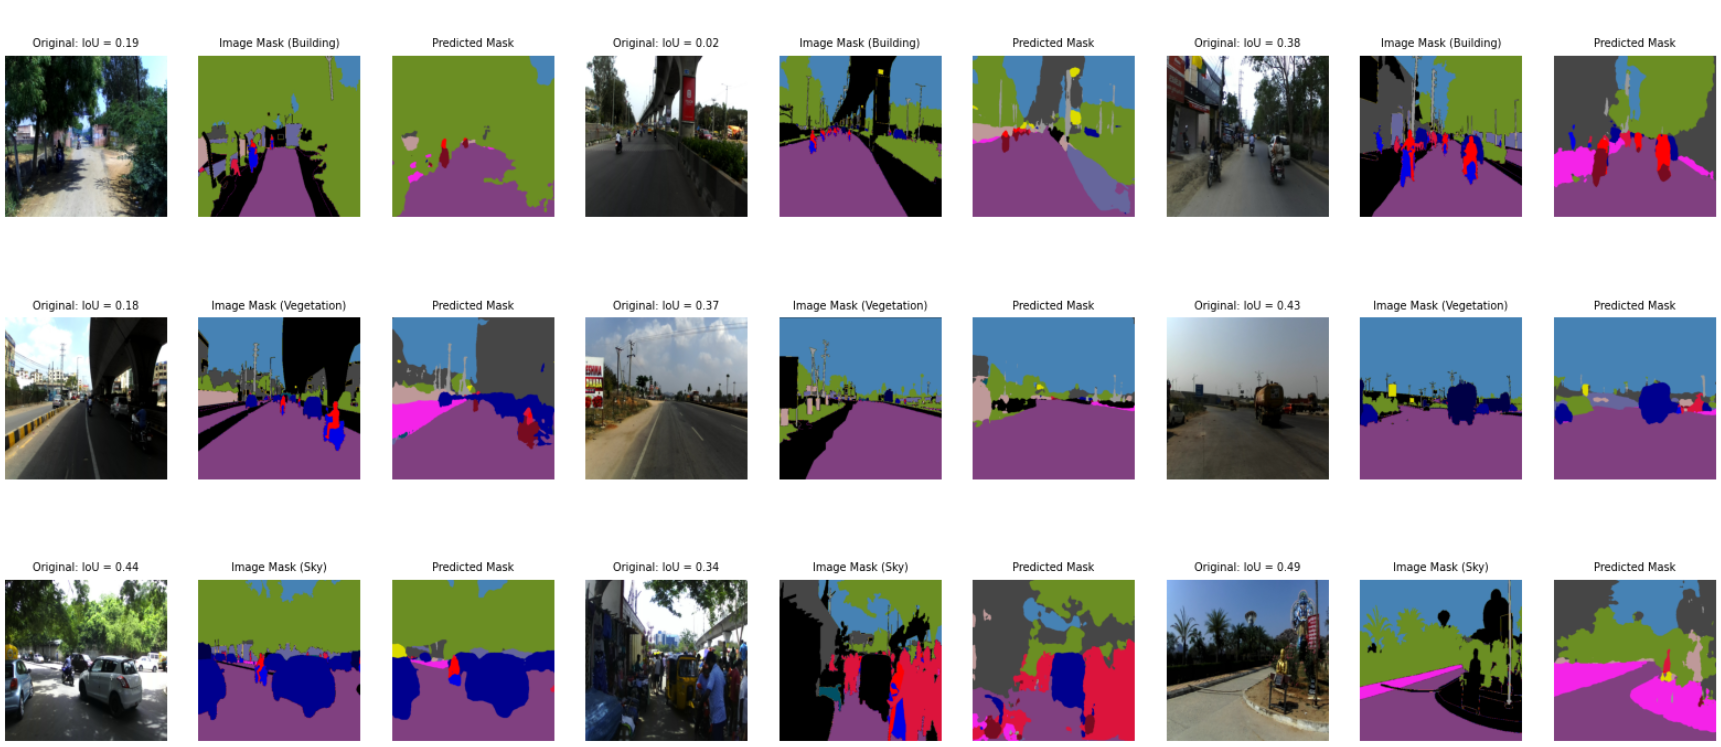
\includegraphics[width=0.325\textwidth]{Assets/Segmentation/Bad-IoUs/06}
            \caption{Examples of three images from each class with IoU $\leq$ 0.5}
            \label{fig:bad-ious}
        \end{figure}
    \end{enumerate}

    \subsection*{\textbf{Question 3.}}
    \begin{enumerate}[label=(\alph*)]
        \item The confusion matrix for the final segmentation was generated and is given in Figure
        (\ref{fig:deeplab-conf-matrix}). We can infer that classes like \texttt{Road} and \texttt{Sky} are being predicted well,
        but others were not - this is seen due to the low count of true positives on the diagonals
        corresponding to these classes. It is also noticable that most mistakes are being made in
        less frequent classes, which are being predicted as classes which are more prevalent.
        \begin{figure}[h!]
            \centering
            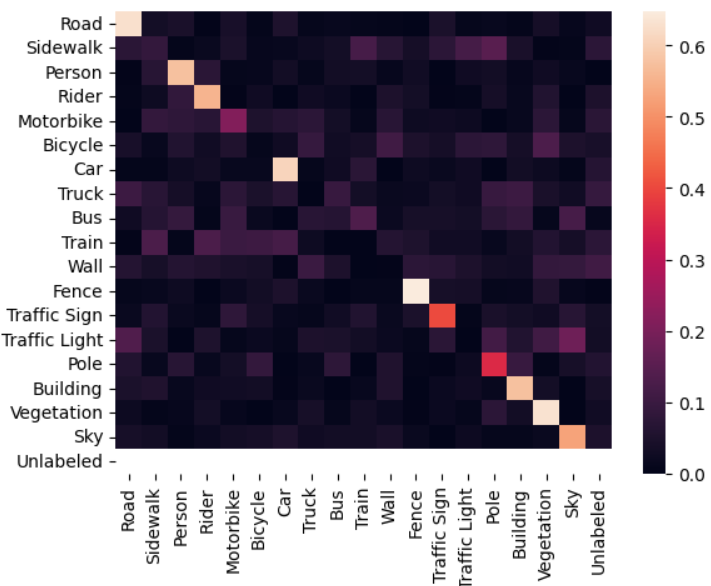
\includegraphics[width=0.5\textwidth]{Assets/Segmentation/Metrics/05}
            \caption{Confusion Matrix for Image Segmentation on Indian Driving Dataset}
            \label{fig:deeplab-conf-matrix}
        \end{figure}
        \item The classwise precision, recall, and F1-scores were calculated and are given in Figure
        (\ref{fig:precision-recall-f1-screenshot}) (again, owing to the lack of time to present the
        results better). Again, it is clear that the model needs improvements in classes which occur
        on a small fraction of an image, for example classes like \texttt{Sidewalk}, \texttt{Train},
        \texttt{Wall}, \texttt{Pole}, etc.
        \begin{figure}[h!]
            \centering
            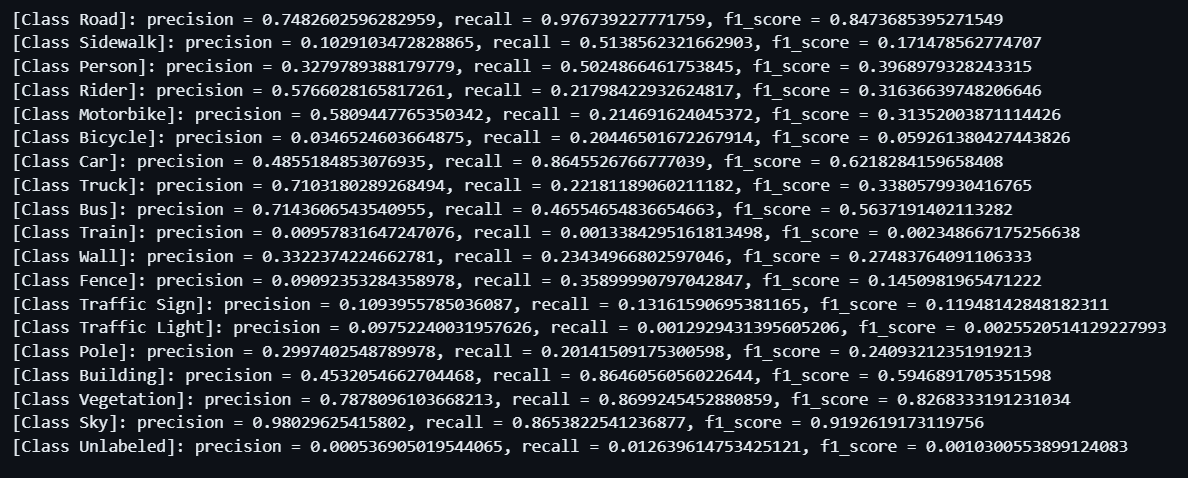
\includegraphics[width=0.5\textwidth]{Assets/Segmentation/Metrics/04}
            \caption{Confusion Matrix for Image Segmentation on Indian Driving Dataset}
            \label{fig:precision-recall-f1-screenshot}
        \end{figure}
    \end{enumerate}

    \subsection*{\textbf{Question 4.}}
    \begin{enumerate}[label=(\alph*)]
        \item The GPU enabled notebook was used to perform inference on the Cityscapes dataset. Like before,
        the generated masks were stored in Google Drive.
        \item Figure (\ref{fig:deeplab-2-conf-matrix}) shows the confusion matrix for these inferences, which are arguably better
        than the previous case. This is because the model was trained on Cityscapes dataset, and is hence able
        to recognize classes better. Now, more classes have a higher count of true positives (diagonal entries
        in the confusion matrix).
        \begin{figure}[h!]
            \centering
            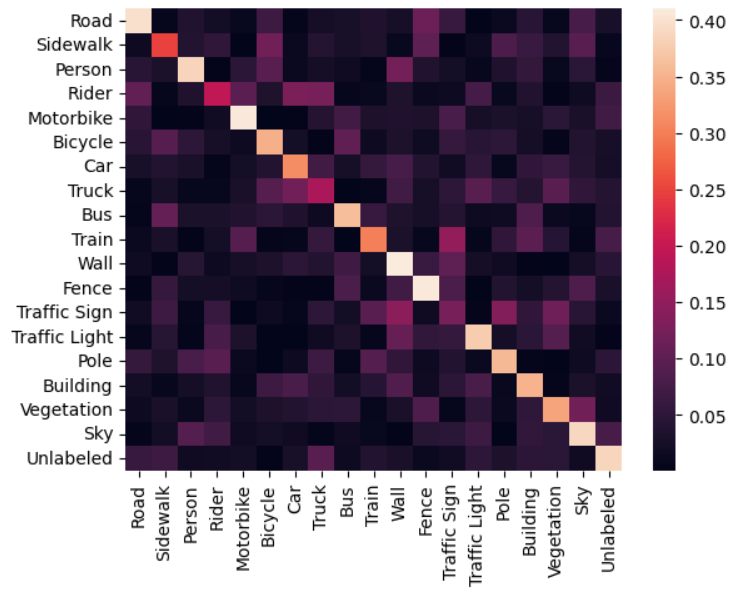
\includegraphics[width=0.5\textwidth]{Assets/Segmentation/Metrics/06}
            \caption{Confusion Matrix for Image Segmentation on Cityscapes Dataset}
            \label{fig:deeplab-2-conf-matrix}
        \end{figure}
        \item Similar to before, the worst performing class performs bad because it is being dominated by
        their environments containing classes like \texttt{Road}, \texttt{Vegetation}, and \texttt{Sky} -
        which span a larger area. Exactly these dominating classes perform well, since they were being predicted
        \textit{more often} in a sense, and covering most of their true pixels. The best performing classes are
        clearly \texttt{Road}, followed by \texttt{Sky} and \texttt{Vegetation}. The worst performing
        classes are \texttt{Traffic\_Sign} and \texttt{Truck}.
    \end{enumerate}

\end{document}